\documentclass[]{book}
\usepackage{lmodern}
\usepackage{amssymb,amsmath}
\usepackage{ifxetex,ifluatex}
\usepackage{fixltx2e} % provides \textsubscript
\ifnum 0\ifxetex 1\fi\ifluatex 1\fi=0 % if pdftex
  \usepackage[T1]{fontenc}
  \usepackage[utf8]{inputenc}
\else % if luatex or xelatex
  \ifxetex
    \usepackage{mathspec}
  \else
    \usepackage{fontspec}
  \fi
  \defaultfontfeatures{Ligatures=TeX,Scale=MatchLowercase}
\fi
% use upquote if available, for straight quotes in verbatim environments
\IfFileExists{upquote.sty}{\usepackage{upquote}}{}
% use microtype if available
\IfFileExists{microtype.sty}{%
\usepackage{microtype}
\UseMicrotypeSet[protrusion]{basicmath} % disable protrusion for tt fonts
}{}
\usepackage{hyperref}
\hypersetup{unicode=true,
            pdftitle={Online R Course},
            pdfborder={0 0 0},
            breaklinks=true}
\urlstyle{same}  % don't use monospace font for urls
\usepackage{natbib}
\bibliographystyle{apalike}
\usepackage{color}
\usepackage{fancyvrb}
\newcommand{\VerbBar}{|}
\newcommand{\VERB}{\Verb[commandchars=\\\{\}]}
\DefineVerbatimEnvironment{Highlighting}{Verbatim}{commandchars=\\\{\}}
% Add ',fontsize=\small' for more characters per line
\usepackage{framed}
\definecolor{shadecolor}{RGB}{248,248,248}
\newenvironment{Shaded}{\begin{snugshade}}{\end{snugshade}}
\newcommand{\AlertTok}[1]{\textcolor[rgb]{0.94,0.16,0.16}{#1}}
\newcommand{\AnnotationTok}[1]{\textcolor[rgb]{0.56,0.35,0.01}{\textbf{\textit{#1}}}}
\newcommand{\AttributeTok}[1]{\textcolor[rgb]{0.77,0.63,0.00}{#1}}
\newcommand{\BaseNTok}[1]{\textcolor[rgb]{0.00,0.00,0.81}{#1}}
\newcommand{\BuiltInTok}[1]{#1}
\newcommand{\CharTok}[1]{\textcolor[rgb]{0.31,0.60,0.02}{#1}}
\newcommand{\CommentTok}[1]{\textcolor[rgb]{0.56,0.35,0.01}{\textit{#1}}}
\newcommand{\CommentVarTok}[1]{\textcolor[rgb]{0.56,0.35,0.01}{\textbf{\textit{#1}}}}
\newcommand{\ConstantTok}[1]{\textcolor[rgb]{0.00,0.00,0.00}{#1}}
\newcommand{\ControlFlowTok}[1]{\textcolor[rgb]{0.13,0.29,0.53}{\textbf{#1}}}
\newcommand{\DataTypeTok}[1]{\textcolor[rgb]{0.13,0.29,0.53}{#1}}
\newcommand{\DecValTok}[1]{\textcolor[rgb]{0.00,0.00,0.81}{#1}}
\newcommand{\DocumentationTok}[1]{\textcolor[rgb]{0.56,0.35,0.01}{\textbf{\textit{#1}}}}
\newcommand{\ErrorTok}[1]{\textcolor[rgb]{0.64,0.00,0.00}{\textbf{#1}}}
\newcommand{\ExtensionTok}[1]{#1}
\newcommand{\FloatTok}[1]{\textcolor[rgb]{0.00,0.00,0.81}{#1}}
\newcommand{\FunctionTok}[1]{\textcolor[rgb]{0.00,0.00,0.00}{#1}}
\newcommand{\ImportTok}[1]{#1}
\newcommand{\InformationTok}[1]{\textcolor[rgb]{0.56,0.35,0.01}{\textbf{\textit{#1}}}}
\newcommand{\KeywordTok}[1]{\textcolor[rgb]{0.13,0.29,0.53}{\textbf{#1}}}
\newcommand{\NormalTok}[1]{#1}
\newcommand{\OperatorTok}[1]{\textcolor[rgb]{0.81,0.36,0.00}{\textbf{#1}}}
\newcommand{\OtherTok}[1]{\textcolor[rgb]{0.56,0.35,0.01}{#1}}
\newcommand{\PreprocessorTok}[1]{\textcolor[rgb]{0.56,0.35,0.01}{\textit{#1}}}
\newcommand{\RegionMarkerTok}[1]{#1}
\newcommand{\SpecialCharTok}[1]{\textcolor[rgb]{0.00,0.00,0.00}{#1}}
\newcommand{\SpecialStringTok}[1]{\textcolor[rgb]{0.31,0.60,0.02}{#1}}
\newcommand{\StringTok}[1]{\textcolor[rgb]{0.31,0.60,0.02}{#1}}
\newcommand{\VariableTok}[1]{\textcolor[rgb]{0.00,0.00,0.00}{#1}}
\newcommand{\VerbatimStringTok}[1]{\textcolor[rgb]{0.31,0.60,0.02}{#1}}
\newcommand{\WarningTok}[1]{\textcolor[rgb]{0.56,0.35,0.01}{\textbf{\textit{#1}}}}
\usepackage{longtable,booktabs}
\usepackage{graphicx,grffile}
\makeatletter
\def\maxwidth{\ifdim\Gin@nat@width>\linewidth\linewidth\else\Gin@nat@width\fi}
\def\maxheight{\ifdim\Gin@nat@height>\textheight\textheight\else\Gin@nat@height\fi}
\makeatother
% Scale images if necessary, so that they will not overflow the page
% margins by default, and it is still possible to overwrite the defaults
% using explicit options in \includegraphics[width, height, ...]{}
\setkeys{Gin}{width=\maxwidth,height=\maxheight,keepaspectratio}
\IfFileExists{parskip.sty}{%
\usepackage{parskip}
}{% else
\setlength{\parindent}{0pt}
\setlength{\parskip}{6pt plus 2pt minus 1pt}
}
\setlength{\emergencystretch}{3em}  % prevent overfull lines
\providecommand{\tightlist}{%
  \setlength{\itemsep}{0pt}\setlength{\parskip}{0pt}}
\setcounter{secnumdepth}{5}
% Redefines (sub)paragraphs to behave more like sections
\ifx\paragraph\undefined\else
\let\oldparagraph\paragraph
\renewcommand{\paragraph}[1]{\oldparagraph{#1}\mbox{}}
\fi
\ifx\subparagraph\undefined\else
\let\oldsubparagraph\subparagraph
\renewcommand{\subparagraph}[1]{\oldsubparagraph{#1}\mbox{}}
\fi

%%% Use protect on footnotes to avoid problems with footnotes in titles
\let\rmarkdownfootnote\footnote%
\def\footnote{\protect\rmarkdownfootnote}

%%% Change title format to be more compact
\usepackage{titling}

% Create subtitle command for use in maketitle
\providecommand{\subtitle}[1]{
  \posttitle{
    \begin{center}\large#1\end{center}
    }
}

\setlength{\droptitle}{-2em}

  \title{Online R Course}
    \pretitle{\vspace{\droptitle}\centering\huge}
  \posttitle{\par}
    \author{}
    \preauthor{}\postauthor{}
    \date{}
    \predate{}\postdate{}
  
\usepackage{booktabs}
\usepackage{amsthm}
\makeatletter
\def\thm@space@setup{%
  \thm@preskip=8pt plus 2pt minus 4pt
  \thm@postskip=\thm@preskip
}
\makeatother

\begin{document}
\maketitle

{
\setcounter{tocdepth}{1}
\tableofcontents
}
\hypertarget{welcome}{%
\chapter{Welcome!}\label{welcome}}

In this tutorial we will be teaching R from the beginning - showing you how to set up R, building foundational R skills then moving onto how to plot and manage your data. Finally, we will introduce modelling in R.

We have written the tutorial in a \textbf{problem-orientated style}. Each chapter will introduce a problem and then we will use \texttt{R} to solve the problem. We have taken this approach as it should hopefully provide you with a context to approach your own problems with and, ideally, by the end of this tutorial, you will have learned enough to apply your skills to your own research questions and data.

We don't expect you to have memorised everything in these tutorials - it's unrealistic and it's not how data analysts work. Our main goal for the end of the tutorial is to teach you where to look and to be able to understand what you find so \textbf{you can learn R yourself} and when your your needs grow, you can solve the problems yourself.

The files for this tutorial are available for your personal use. If you reuse sections of this tutorial, please mention us and the appropriate citations found in the biblography.

If you have any comments or corrections, please contact us through \url{https://stats4sd.org/contact}

\hypertarget{setting-up}{%
\chapter{Setting up}\label{setting-up}}

Unfortunately, as with any new skill, the first chapter can be the most text heavy. Apologies. We will do our best to;

\begin{itemize}
\tightlist
\item
  Keep it as brief as possible
\item
  clearly structured so you can skip sections as needed
\item
  complete so you know that after this chapter you will be focused on coding.
\end{itemize}

\hypertarget{about-r-and-rstudio}{%
\section{About R and RStudio}\label{about-r-and-rstudio}}

\texttt{R} is a progamming language that is primarily focused on statistics. This means that it's a way of talking to your computer to get it to solve certain problems and \texttt{R}'s speciality is statistics and data analysis.

It's not all it can do and is a great pathway to transition from point-and-click data analysis to more general programming. The skills you will learn along the way are part of most modern languages, so your time will be well spent!

There are many reasons individuals use \texttt{R} but for our needs the main selling points are;

\begin{itemize}
\tightlist
\item
  Integrated platform for all data management, analysis and graphics
\item
  Allows for reproducible research
\item
  Active community of users providing support
\item
  Cost = Free!
\end{itemize}

\hypertarget{installing-r-and-rstudio}{%
\subsection{Installing R and RStudio}\label{installing-r-and-rstudio}}

\texttt{R} comes bundled with an interface but not many people use it. The vast majority of \texttt{R} users actually use \textbf{RStudio} to work with R including us. RStudio provides a lot of useful features such as making it easier to see what you've done so far and view the help menu.

There are two options at the time of writing; installing \texttt{R} and RStudio on your personal computer (local) or using an online version (cloud). Either is fine. The cloud version is, at the time of writing, free but this is likely to change. Also the cloud version can be slow. Basically, if you are uncomfortable or unable to install programs on your computer, then use the cloud version. Otherwise, the local version is the best choice.

\hypertarget{local}{%
\subsubsection{Local}\label{local}}

We recommend following the ``Download, Install and Setup R and RStudio'' tutorial on \url{https://www.statslectures.com/r-stats-videos-tutorials/getting-started-with-r}

The direct link is here; \url{https://youtu.be/riONFzJdXcs}

\hypertarget{cloud}{%
\subsubsection{Cloud}\label{cloud}}

As of the time of writing, RStudio is providing a free version of their software that you can run in your web-browser. Go to \url{https://rstudio.cloud} and sign up as you would most online accounts.

One thing to note is getting data onto the cloud requires an extra step. You'll need to press \texttt{Upload} in the bottom right panel, shown below, and browse your computer for the files. Also, if you want to upload multiple files at once, you need to first ``zip'' these files together and upload this file.

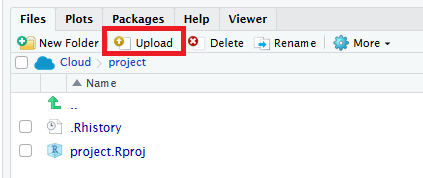
\includegraphics[width=\textwidth,height=\textheight]{Images/rstudio_cloud_upload_button}

\hypertarget{get-the-data}{%
\section{Get the data}\label{get-the-data}}

The data sets can be currently found at the \href{https://stats4sd.org/download/online-r-course_2019-05-14_13:50:11/2019-06-05_12:58:35_data.zip/Data.zip}{following link}.

In case the link is broken, the updated link is likely to be found by navigating to \url{https://stats4sd.org/resources}, searching ``Online R Course'' and downloading \texttt{Data.zip}.

\hypertarget{navigating-rstudio}{%
\section{Navigating RStudio}\label{navigating-rstudio}}

Open RStudio by either opening the program on your computer as you normally would or by going to \url{https://rstudio.cloud}, logging in and then pressing new project.

You will be faced with something like this;

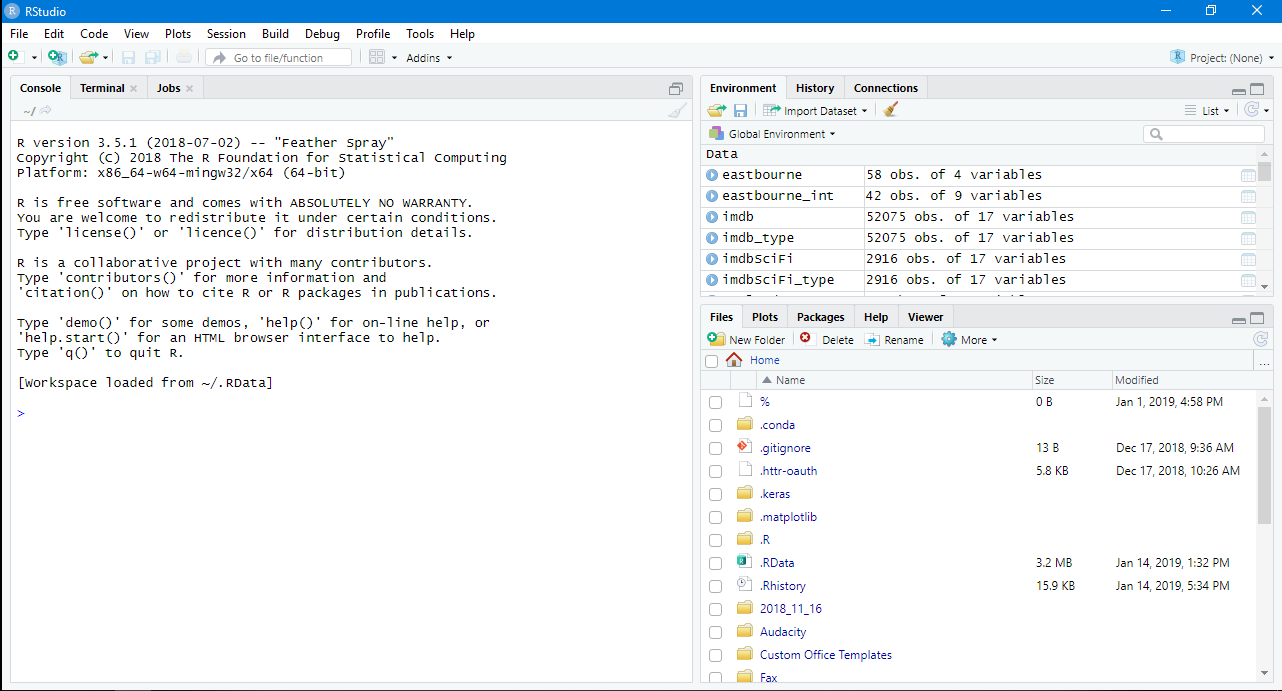
\includegraphics[width=\textwidth,height=\textheight]{Images/RStudio}

If you're overwhelmed by the options, don't worry! We will show where the most important sections.

The first thing to notice is there are three main sections. Each of these sections has ``tabs'' in the same way your web browser does.

\hypertarget{console}{%
\subsection{Console}\label{console}}

The left most and largest section main tab is called ``Console''. This is where you type you R code. For example, type \texttt{2+2} and then press Enter. You've just run your R command.

\hypertarget{environment}{%
\subsection{Environment}\label{environment}}

To the top right there is a single important tab; ``Environment'' which tracks all the things you've made during your current working time with R.

\hypertarget{packages-help}{%
\subsection{Packages, Help}\label{packages-help}}

The bottom right panel has two panels we will use; packages and help. Both will be covered later but briefly packages are where R extensions are listed and Help is where we can access support documents about R in a convenient way.

\hypertarget{source}{%
\subsection{Source}\label{source}}

We are about to introduce our fourth and final panel. Above the ``Console'' there is a button called \texttt{File}. Do the following; \texttt{File\ -\textgreater{}\ New\ File\ -\textgreater{}\ R\ Markdown}. It might take a little while to load the first time as it is setting up, just be patient. We will talk about R Markdown in the next session but a quick note; this new section is generally called ``Source'' because this is the source of the R Code you have written which is then sent to your console.

If you look at the bottom of your window, you should see ``Console'', which was minimised when you opened Source. As you with any other program, to the right you can use the split-screen and maximise button.

To recap, the main tabs you need to know are ``Console'', ``Environment'', ``Help'', ``Source'', and ``Packages''

\textbf{QUESTION: Can you open each of these panels?}

\hypertarget{r-markdown}{%
\section{R Markdown}\label{r-markdown}}

R Markdown are documents that allow you to write text around your code and output your work into multipile formats, including a HTML, PDF or Word.

The ``text mode'' is similar to your experience with typing documents in Word or Notepad. Technically it uses ``Markdown'', so you have the option for tables and numbered lists in your final output.

Code in R Markdown is implemented in ``chunks''. There are two types of chunks, in-line and blocks. To insert a chunk, you need to press \texttt{Insert\ -\textgreater{}\ R} located at the top right of the ``Source'' panel.

Once done, enter the code below and press the green play button on the right hand side of the chunk. In this tutorial, code appears in a light grey box and output in a white box.

\textbf{Code}

\begin{Shaded}
\begin{Highlighting}[]
\DecValTok{2}\OperatorTok{+}\DecValTok{2}
\end{Highlighting}
\end{Shaded}

\textbf{Output}

\begin{verbatim}
## [1] 4
\end{verbatim}

Hopefully when you run the code, you see that 2+2 still equals 4!

The code chunks in R Markdown start with \texttt{\textasciigrave{}\textasciigrave{}\textasciigrave{}\{r\}} and ends with \texttt{\textasciigrave{}\textasciigrave{}\textasciigrave{}}.

Do not modify these lines of the chunk otherwise bad things might happen. Modify anything in the middle.

\hypertarget{comments}{%
\section{Comments}\label{comments}}

Using \texttt{\#} in a code block stops the anything after the symbol being run. \texttt{\#} is referred to as ``commenting'' code because it's usually used to add commentry to long pieces of code. Try running the code below.

\textbf{QUESTION: What do you think the code below will output? Why?}

\begin{Shaded}
\begin{Highlighting}[]
\CommentTok{#I am trying to calculate the following;}
\DecValTok{2} \OperatorTok{+}\StringTok{ }\DecValTok{2} \CommentTok{# + 2}
\CommentTok{# + two}
\end{Highlighting}
\end{Shaded}

\hypertarget{getting-the-files}{%
\section{Getting the files}\label{getting-the-files}}

For this tutorial you will need to download a collection of files. These can be found at \href{https://stats4sd.org/download/online-r-course_2019-05-14_13:50:11/2019-06-05_12:58:35_data.zip/Data.zip}{here}. One you have downloaded them, you will need to extract them.

\hypertarget{base-r}{%
\chapter{Base-R}\label{base-r}}

Congratulations! By this point you should have successfully installed R and R Studio. If not, see the previous chapter.

Specifically you have installed ``Base-R''. R is an extendable language, which means you can expand it's vocabulary to solve problems in new and simplier ways. It's why it's so fresh and on the cuting edge.

In this tutorial, we're going to start with the standard language; ``Base-R''. It also provides the foundation for later topics. ``Base-R'' is by no means basic! There are many people who only use base-r for the entirety of their projects. It's \textbf{Base}-R not \textbf{Basic}-R.

\hypertarget{objects-and-functions}{%
\section{Objects and functions}\label{objects-and-functions}}

Within R there are two fundemental concepts; objects and functions. Objects are a way of holding information. Functions are a way of manipulating objects. This may seem really complicated but the code below demonstrates this concept.

\begin{Shaded}
\begin{Highlighting}[]
\DecValTok{2}\OperatorTok{+}\DecValTok{2}
\end{Highlighting}
\end{Shaded}

\begin{verbatim}
## [1] 4
\end{verbatim}

\textbf{QUESTION: In this example there are 2 objects and 1 function. Can you name them?}

.

.

.

The objects are \texttt{2,\ 2} and the function is \texttt{+}.

To create custom objects in R we use \texttt{\textless{}-}, pronounced ``assign''.

\begin{Shaded}
\begin{Highlighting}[]
\NormalTok{x <-}\StringTok{ }\DecValTok{2}\OperatorTok{+}\DecValTok{2}
\end{Highlighting}
\end{Shaded}

This would read as ``assign the object \texttt{x} the value of 2+2''.

What do you see underneath the chunk this time? Does 2+2 no longer = 4?

When objects are assigned they usually do not return any output directly. Check over in the Environment pane of RStudio on the right hand side of the screen?

Can you see something called x? What does the environment say about x?

You could also print this out more explicitly by submitting the name of the object in an R chunk.

\begin{Shaded}
\begin{Highlighting}[]
\NormalTok{x}
\end{Highlighting}
\end{Shaded}

\begin{verbatim}
## [1] 4
\end{verbatim}

If you skipped the previous chunk (because it seemed obvious - you know what 2+2 is!) you might have got an error. You need to create an object x before you can look at it. If you missed running a previous chunk, or like skipping to the end then you can press the button to the left of the play button ``run all chunks above'' (grey triangle above a green line)

\hypertarget{naming-objects}{%
\subsection{Naming objects}\label{naming-objects}}

When giving things names in R it is better to be a bit more informative than using single letters (x,y,z etc.).
We can give R objects any name we want to - but there are a few rules:
1. No punctuation except \_ and .
2. No spaces
3. Only standard english alphanumeric characters - no accents
4. Names can include numbers but can't start with numbers

This is valid

\begin{Shaded}
\begin{Highlighting}[]
\NormalTok{sjkfjhskjdhsajsfgldsjghajfhljhgsdlk <-}\StringTok{ }\DecValTok{2}\OperatorTok{+}\DecValTok{2}
\end{Highlighting}
\end{Shaded}

But really stupid - we want our names to be short, clear and memorable

\hypertarget{errors}{%
\subsection{Errors}\label{errors}}

R is also case sensitive - try running this:

\begin{Shaded}
\begin{Highlighting}[]
\NormalTok{X}
\end{Highlighting}
\end{Shaded}

\begin{verbatim}
## Error in eval(expr, envir, enclos): object 'X' not found
\end{verbatim}

Get used to that error! We have an object called \texttt{x} but we don't have anything called \texttt{X}. Capitalisation and spelling is vital.

As a new user remember that about most of your initial errors are likely to be found by checking the \textbf{B.S.Q.C. (brackets; spelling; quotation marks; case)}, or the result of problems with sequencing of loading data or packages.

Its also a good idea to avoid names which are used elsewhere in R for functions as this can cause problems with duplication and/or confusion.

R is big so there are lots of names used for things, so sometimes it happens but try to avoid as much as possible.

Speaking of functions\ldots{}

\hypertarget{functions}{%
\section{Functions}\label{functions}}

A function is something that takes in a thing (input) and returns a thing (output). Nearly all functions get called like this

\texttt{functionname(input)}

Most functions also work like this
\texttt{functionname(input\_1,\ input\_2,\ ...)}

A super useful function is c() and is everywhere is R, but does not have a very informative name. It is short for \textbf{c}ombine since it \textbf{c}ombines a bunch of stuff together.

\begin{Shaded}
\begin{Highlighting}[]
\KeywordTok{c}\NormalTok{(}\DecValTok{1}\NormalTok{,}\DecValTok{2}\NormalTok{,}\DecValTok{3}\NormalTok{,}\DecValTok{4}\NormalTok{,}\DecValTok{5}\NormalTok{)}
\end{Highlighting}
\end{Shaded}

\begin{verbatim}
## [1] 1 2 3 4 5
\end{verbatim}

Think of \texttt{c()} taking the inputs and making a list from them. In our example, the first item in the list is \texttt{1}, the second being \texttt{2}, ect.

Question: Modify the chunk above so that this is assigned to an object called y

You could now use another function to get ther average of those numbers

\begin{Shaded}
\begin{Highlighting}[]
\KeywordTok{mean}\NormalTok{(y)}
\end{Highlighting}
\end{Shaded}

\begin{verbatim}
## Error in mean(y): object 'y' not found
\end{verbatim}

Remember - this line will only work if you succesfully assigned the object y.

\begin{Shaded}
\begin{Highlighting}[]
\NormalTok{y<-}\KeywordTok{c}\NormalTok{(}\DecValTok{1}\NormalTok{,}\DecValTok{2}\NormalTok{,}\DecValTok{3}\NormalTok{,}\DecValTok{4}\NormalTok{,}\DecValTok{5}\NormalTok{)}
\KeywordTok{mean}\NormalTok{(y)}
\end{Highlighting}
\end{Shaded}

\begin{verbatim}
## [1] 3
\end{verbatim}

\hypertarget{help}{%
\subsection{Help}\label{help}}

Throughout this tutorial you will be introduced to a lot of new functions with even more options. \textbf{We don't expect you to memorise them}. You are learning \textbf{where} to look.

You can get help within R by using a question mark followed by the name of the function.

\begin{Shaded}
\begin{Highlighting}[]
\NormalTok{?mean}
\end{Highlighting}
\end{Shaded}

The help files will list the options and a brief description. Once you know what you are looking for, it's easy to read.

There are always worked examples in the help file along with each function, which are often more useful than the help menus themselves. This can be found using \texttt{example()}

\begin{Shaded}
\begin{Highlighting}[]
\KeywordTok{example}\NormalTok{(mean)}
\end{Highlighting}
\end{Shaded}

\begin{verbatim}
## 
## mean> x <- c(0:10, 50)
## 
## mean> xm <- mean(x)
## 
## mean> c(xm, mean(x, trim = 0.10))
## [1] 8.75 5.50
\end{verbatim}

But \texttt{?} and \texttt{example()} only work if you know the name of the function!

There are other ways of checking within R for how to do things; but at this point you are much better off heading to Google.

\url{https://www.google.co.uk/search?q=How+do+I+calculate+a+mean+in+R}

\hypertarget{packages}{%
\section{Packages}\label{packages}}

Up to this point, we've been using Base-R.

A really nice thing about R is that anyone can write extensions to R called packages. There are lots of really useful packages that make working with R much easier, others that let you make really nice graphics, or fit clever statistical models.

In this course we will use some of these packages so let's set up now by making sure we have everything we need. To get them we need to download them from the internet and install them into our version of R. To do so, run the following code;

\begin{Shaded}
\begin{Highlighting}[]
\KeywordTok{install.packages}\NormalTok{(}\KeywordTok{c}\NormalTok{(}\StringTok{"ggplot2"}\NormalTok{,}\StringTok{"dplyr"}\NormalTok{,}\StringTok{"openxlsx"}\NormalTok{, }\StringTok{"tidyr"}\NormalTok{, }\StringTok{"plotly"}\NormalTok{))}
\end{Highlighting}
\end{Shaded}

We will talk about these packages when we need them later - don't worry too much about what each of them do for now.

\hypertarget{quotation-marks}{%
\section{Quotation Marks}\label{quotation-marks}}

Also note that each of the packages in the previous line are in quotation marks. This is because they are not things that exist in our current session of R (yet).

Look at the difference between these two lines

\begin{Shaded}
\begin{Highlighting}[]
\NormalTok{x}
\end{Highlighting}
\end{Shaded}

\begin{verbatim}
##  [1]  0  1  2  3  4  5  6  7  8  9 10 50
\end{verbatim}

\begin{Shaded}
\begin{Highlighting}[]
\StringTok{"x"}
\end{Highlighting}
\end{Shaded}

\begin{verbatim}
## [1] "x"
\end{verbatim}

Something in quotation marks is treated literally as what is there.
Something not in quotation marked is evaluated.

If we use the name of something not in quotation marks and it is not the name of something already in our R session we get an error

\hypertarget{graphics-with-ggplot2}{%
\chapter{Graphics with ggplot2}\label{graphics-with-ggplot2}}

\hypertarget{welcome-to-ggplot}{%
\section{Welcome to ggplot}\label{welcome-to-ggplot}}

Graphs play an important part of any data analysis in understanding your data.

As we've mentioned in the previous chapter, \texttt{base-R} can be extended using packages and the particular package we'll be using in this tutorial will be \texttt{ggplot2} \citep{R-ggplot2}.

There are lots of of different systems for producing graphs in R. We are going to focus on the \texttt{ggplot2} package. The syntax can look scary at first, but once you understand the basic building blocks, you will be able to produce complex graphs very easily.

Comparing \texttt{base-R} with \texttt{ggplot2}

\textbf{baseR}

\begin{itemize}
\tightlist
\item
  Simple intuitive syntax for basic plot\\
\item
  Pretty ugly basic plot\\
\item
  Inconsistent syntax for different plot types\\
\item
  Complicated syntax for customisation
\end{itemize}

\textbf{ggplot2}

\begin{itemize}
\tightlist
\item
  Unusual syntax for basic plot\\
\item
  Pretty looking basic plot\\
\item
  Consistent syntax for different plot types\\
\item
  Consistent syntax for customisation
\end{itemize}

1 against 3. ggplot2 wins.

\hypertarget{ggplot2_setting_up}{%
\section{Setting up}\label{ggplot2_setting_up}}

Assuming you have followed the previous chapter, particularly from \ref{installing-r-and-rstudio}, at this stage you have installed \texttt{R}, RStudio, familarised yourself with the key panels and then installed key packages including \texttt{ggplot2}.

This means you simply need to load \texttt{ggplot2} into your current session by simply running the command below.

\begin{Shaded}
\begin{Highlighting}[]
\KeywordTok{library}\NormalTok{(ggplot2)}
\end{Highlighting}
\end{Shaded}

To plot our data, we first need data. Luckily we have some prepared for you.

The simpliest way for this tutorial is to look at the \texttt{Environment} panel in the top right of RStudio and press the folder with the green arrow. Navigate to the Data folder you downloaded from GitHub (Link Here). Double click on \texttt{03\ Pulse.RData}. In a later chapter, we will talk about how to import other formats.

\hypertarget{description-of-the-pulse-of-the-nation-dataset}{%
\section{Description of the ``Pulse of the Nation'' Dataset}\label{description-of-the-pulse-of-the-nation-dataset}}

Before we proceed with any analysis, and even outside this tutorial, it is important to understand your dataset.

You can view the dataset in RStudio by single clicking the name in the Environment tab.

The ``Pulse'' dataset is an extract from the monthly survey ``Pulse of the Nation'' made by Cards Against Humanity \citep{pulse} which contains a representative sample of US citizens.The dataset contains an extract of 356 repsonses to 10 of the survey questions:

\begin{longtable}[]{@{}ll@{}}
\toprule
\begin{minipage}[b]{0.11\columnwidth}\raggedright
\textbf{Variable}\strut
\end{minipage} & \begin{minipage}[b]{0.83\columnwidth}\raggedright
\textbf{Question}\strut
\end{minipage}\tabularnewline
\midrule
\endhead
\begin{minipage}[t]{0.11\columnwidth}\raggedright
Gender\strut
\end{minipage} & \begin{minipage}[t]{0.83\columnwidth}\raggedright
What gender do you identify with?\strut
\end{minipage}\tabularnewline
\begin{minipage}[t]{0.11\columnwidth}\raggedright
Age\strut
\end{minipage} & \begin{minipage}[t]{0.83\columnwidth}\raggedright
What is your age?\strut
\end{minipage}\tabularnewline
\begin{minipage}[t]{0.11\columnwidth}\raggedright
AgeGrp\strut
\end{minipage} & \begin{minipage}[t]{0.83\columnwidth}\raggedright
Age range\strut
\end{minipage}\tabularnewline
\begin{minipage}[t]{0.11\columnwidth}\raggedright
Race\strut
\end{minipage} & \begin{minipage}[t]{0.83\columnwidth}\raggedright
What is your race?\strut
\end{minipage}\tabularnewline
\begin{minipage}[t]{0.11\columnwidth}\raggedright
Income\strut
\end{minipage} & \begin{minipage}[t]{0.83\columnwidth}\raggedright
About how much money do you make per year? (USD)\strut
\end{minipage}\tabularnewline
\begin{minipage}[t]{0.11\columnwidth}\raggedright
Education\strut
\end{minipage} & \begin{minipage}[t]{0.83\columnwidth}\raggedright
What is your highest level of education?\strut
\end{minipage}\tabularnewline
\begin{minipage}[t]{0.11\columnwidth}\raggedright
PoliticalParty\strut
\end{minipage} & \begin{minipage}[t]{0.83\columnwidth}\raggedright
In politics today do you consider yourself a Democrat a Republican or Independent?\strut
\end{minipage}\tabularnewline
\begin{minipage}[t]{0.11\columnwidth}\raggedright
PoliticalView\strut
\end{minipage} & \begin{minipage}[t]{0.83\columnwidth}\raggedright
Would you say you are liberal conservative or moderate?\strut
\end{minipage}\tabularnewline
\begin{minipage}[t]{0.11\columnwidth}\raggedright
ApproveTrump\strut
\end{minipage} & \begin{minipage}[t]{0.83\columnwidth}\raggedright
Do you approve disapprove or neither approve nor disapprove of how Donald Trump is handling his job as president?\strut
\end{minipage}\tabularnewline
\begin{minipage}[t]{0.11\columnwidth}\raggedright
Attractiveness\strut
\end{minipage} & \begin{minipage}[t]{0.83\columnwidth}\raggedright
On a scale of 1-10 how physically attractive are you?\strut
\end{minipage}\tabularnewline
\bottomrule
\end{longtable}

\hypertarget{main-components-of-ggplot2}{%
\section{Main components of ggplot2}\label{main-components-of-ggplot2}}

To build a plot in \texttt{ggplot2}, you have to specify features of the plot. The two essential ones are;

\begin{itemize}
\item
  Aesthetics - \texttt{aes()} - describes which variables in our dataset are going to be mapped to what components of our plot
\item
  Geometries - \texttt{geom\_****()} - describes how the variables will be plotted
\end{itemize}

The other types of features are; Scales, Themes, Facets which will be introduced throughout this tutorial.

\hypertarget{first-ggplot2-graph}{%
\section{First ggplot2 graph}\label{first-ggplot2-graph}}

Here is how you produce a scatter plot of perceived attractiveness against age

\begin{Shaded}
\begin{Highlighting}[]
\KeywordTok{ggplot}\NormalTok{(}\DataTypeTok{data =}\NormalTok{ Pulse, }\KeywordTok{aes}\NormalTok{(}\DataTypeTok{x =}\NormalTok{ Attractiveness, }\DataTypeTok{y =}\NormalTok{ Income)) }\OperatorTok{+}\StringTok{ }
\StringTok{  }\KeywordTok{geom_point}\NormalTok{()}
\end{Highlighting}
\end{Shaded}

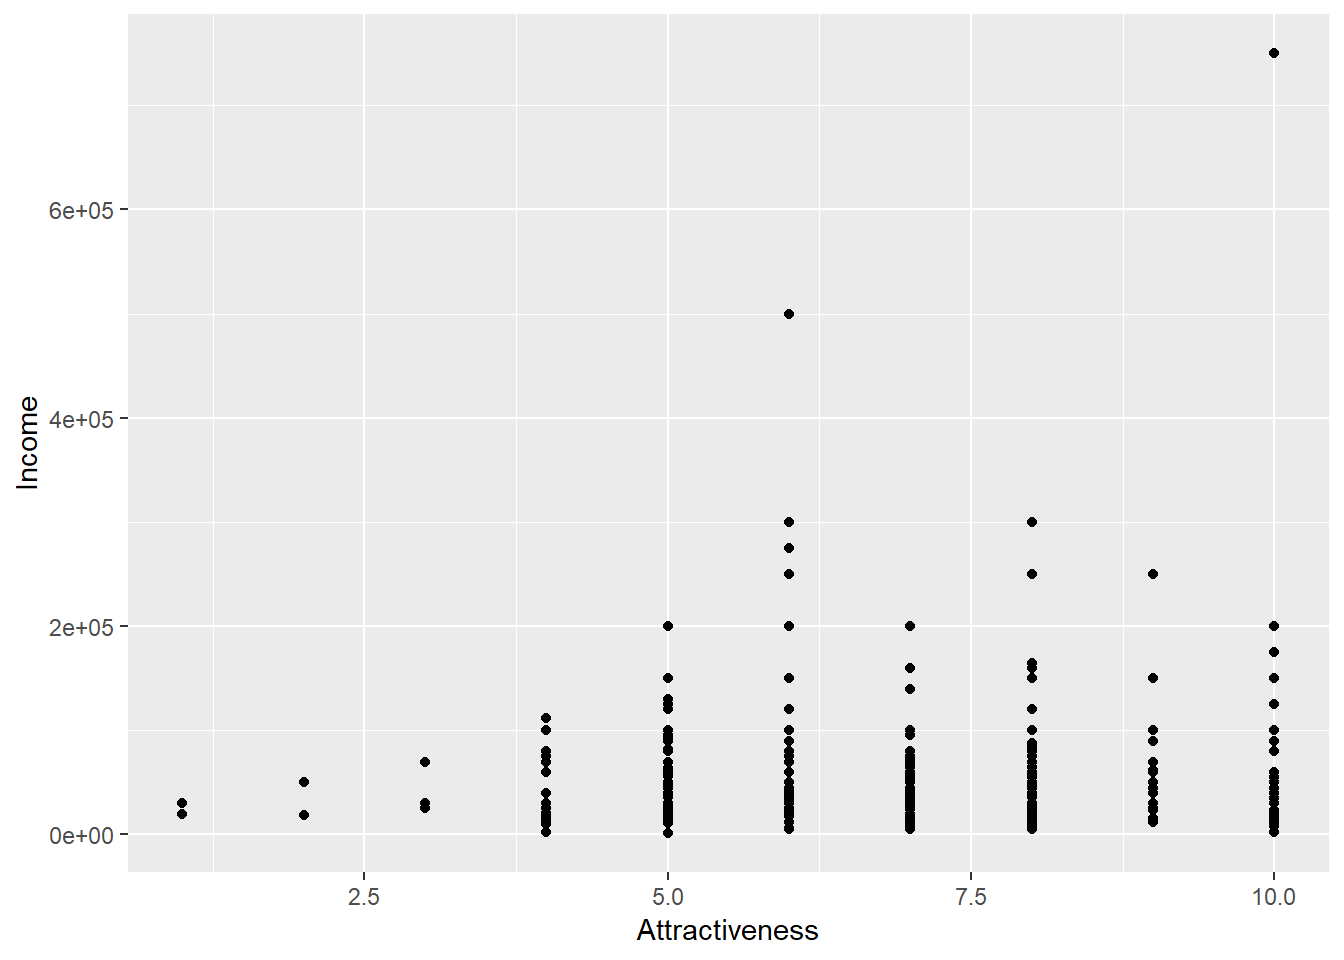
\includegraphics{Online_R_Course_files/figure-latex/unnamed-chunk-23-1.pdf}

Before we break down this example, it is perhaps worth noting the notation used on the y axis. It is how computers show scientific notation where \texttt{2e+05} \(= 2 \times 10^5\).

Now let's look at the different parts of the commands.

With \texttt{ggplot2}, you always begin a graph with the function \texttt{ggplot()}, which creates the base layer and sets the default for each plot but it is blank until we add some layers - ``geoms'' - to it.

The \texttt{aes} argument defines which variables you want to use for which purpose. `\texttt{aes}' is short for aesthetics. So \texttt{ggplot(data\ =\ Pulse,\ aes(x\ =\ Attractiveness,\ y\ =\ Income))} defines the data and the variables to be plotted on the x-axis and the y-axis.

\begin{Shaded}
\begin{Highlighting}[]
\KeywordTok{ggplot}\NormalTok{(}\DataTypeTok{data =}\NormalTok{ Pulse,  }\KeywordTok{aes}\NormalTok{(}\DataTypeTok{x =}\NormalTok{ Attractiveness, }\DataTypeTok{y =}\NormalTok{ Income))}
\end{Highlighting}
\end{Shaded}

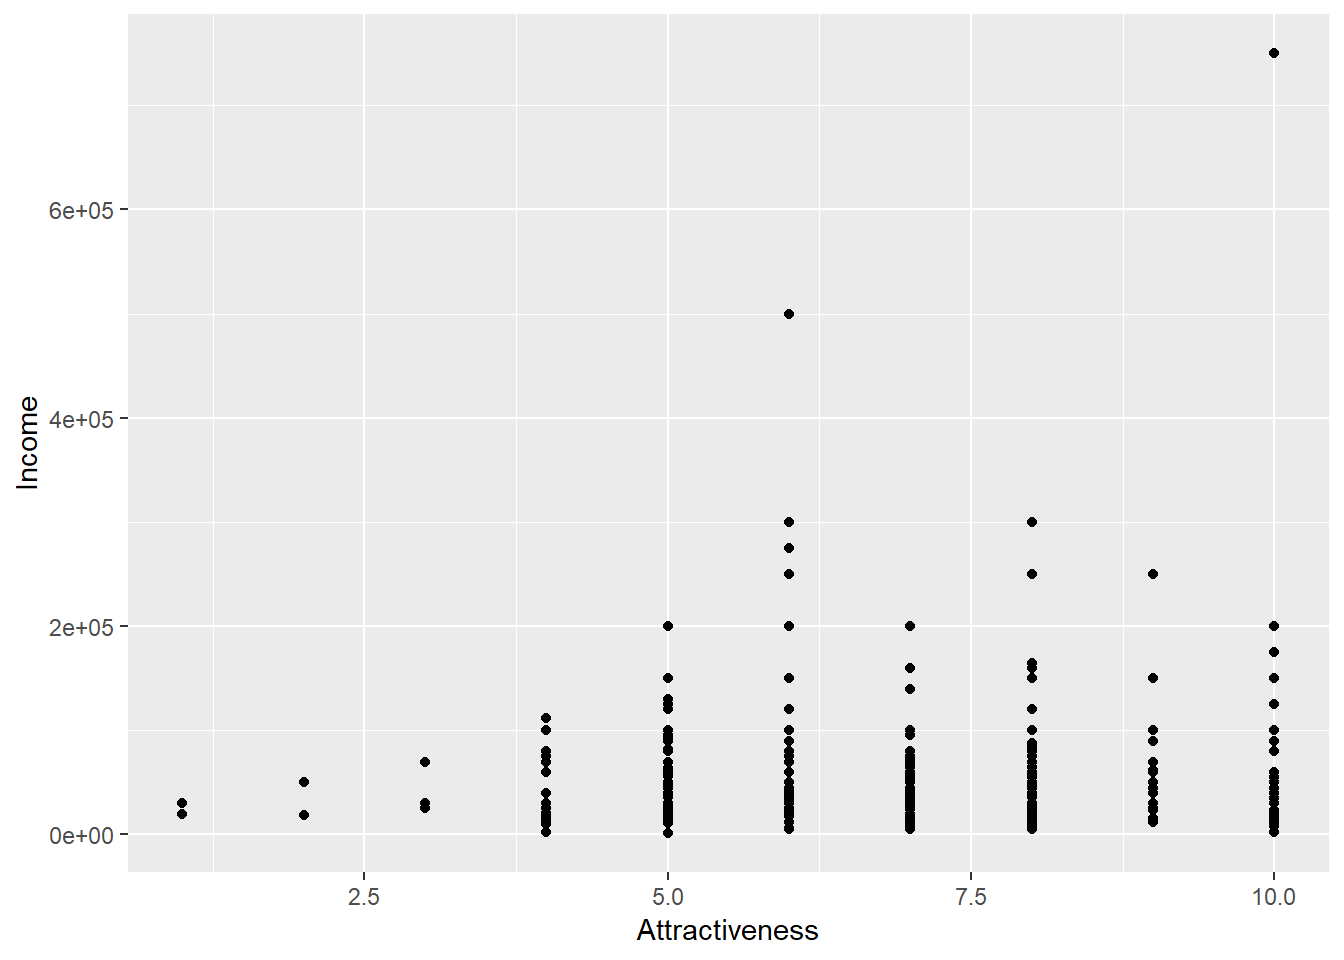
\includegraphics{Online_R_Course_files/figure-latex/unnamed-chunk-24-1.pdf}

As you can see - not a very informative graph!

You complete your graph by adding one or more layers to \texttt{ggplot()}. There are many different types of layers you can use to create your graph and they all start with \texttt{geom\_????}. For example, the function \texttt{geom\_line()} adds a layer of a line to your plot.

\begin{Shaded}
\begin{Highlighting}[]
\KeywordTok{ggplot}\NormalTok{(}\DataTypeTok{data =}\NormalTok{ Pulse,  }\KeywordTok{aes}\NormalTok{(}\DataTypeTok{x =}\NormalTok{ Attractiveness, }\DataTypeTok{y =}\NormalTok{ Income)) }\OperatorTok{+}
\StringTok{  }\KeywordTok{geom_point}\NormalTok{()}
\end{Highlighting}
\end{Shaded}

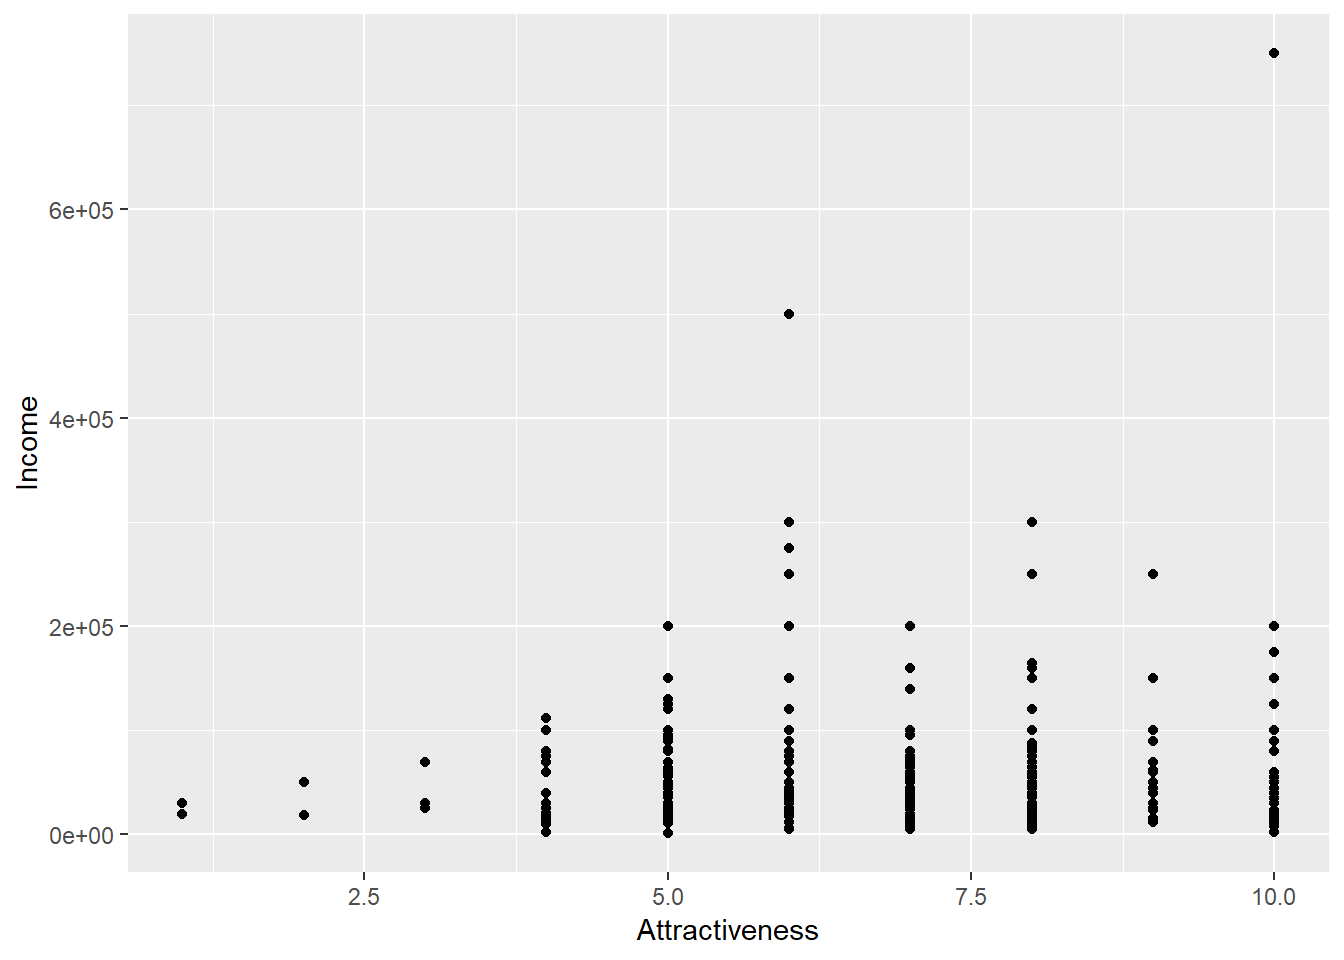
\includegraphics{Online_R_Course_files/figure-latex/unnamed-chunk-25-1.pdf}

\textbf{QUESTION: Modify the same command to instead plot a scatter plot of age on the x axis against income on the y axis}

\hypertarget{adding-colour}{%
\section{Adding colour}\label{adding-colour}}

We can modify the appearance of our points in one of 2 ways - either we can map a variable of our data to an aesthetic or we can permanently apply a style characteristic across all points. To make all the points purple we can add colour=``purple'' into the geom\_point() part of the syntax.

\begin{Shaded}
\begin{Highlighting}[]
\KeywordTok{ggplot}\NormalTok{(}\DataTypeTok{data =}\NormalTok{ Pulse,  }\KeywordTok{aes}\NormalTok{(}\DataTypeTok{x =}\NormalTok{ Attractiveness, }\DataTypeTok{y =}\NormalTok{ Income)) }\OperatorTok{+}\StringTok{ }
\StringTok{  }\KeywordTok{geom_point}\NormalTok{(}\DataTypeTok{colour=}\StringTok{"purple"}\NormalTok{)}
\end{Highlighting}
\end{Shaded}

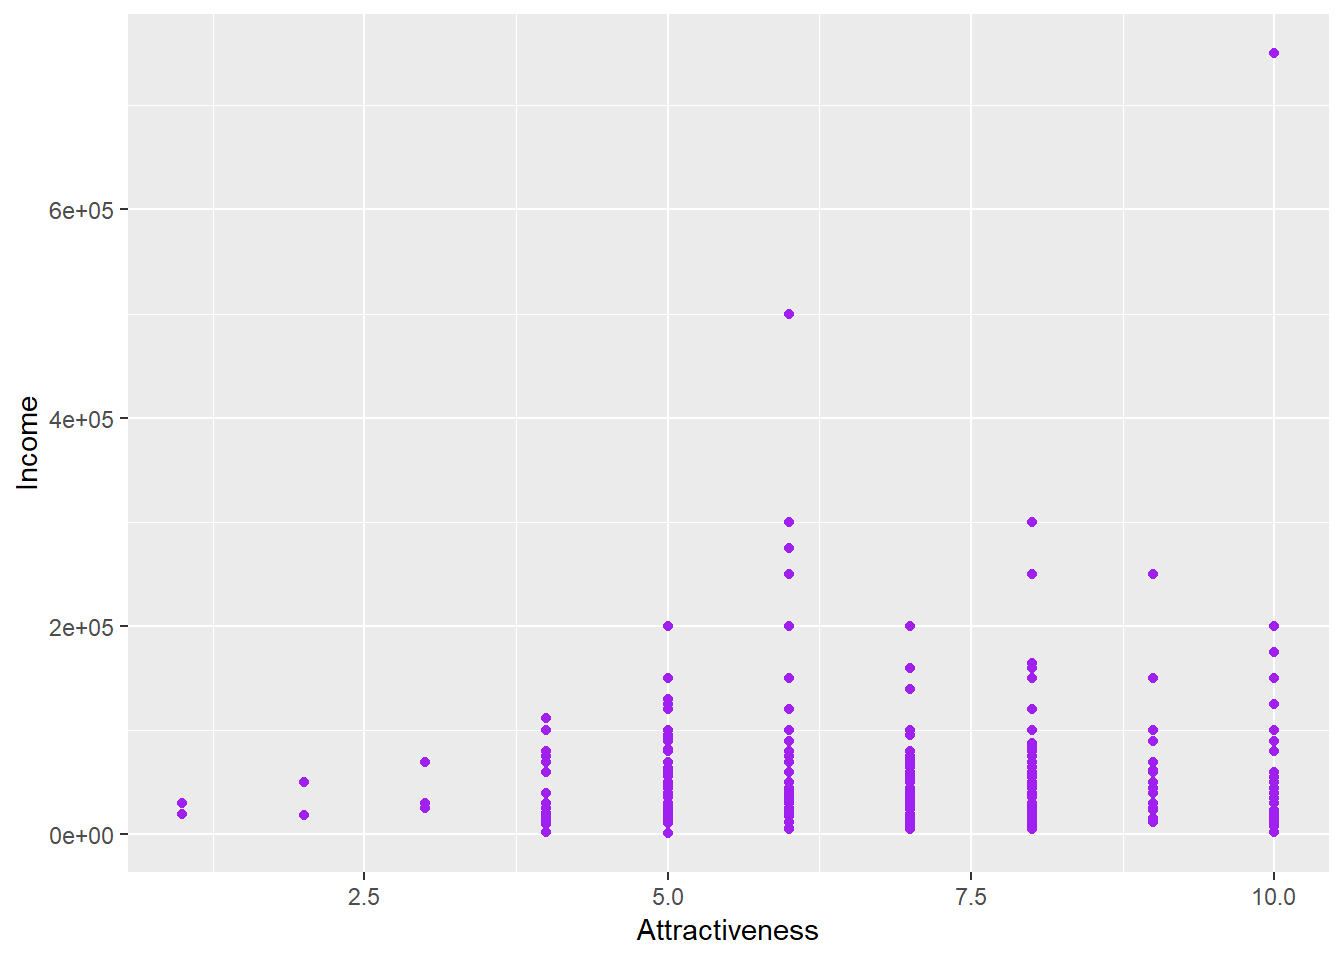
\includegraphics{Online_R_Course_files/figure-latex/unnamed-chunk-26-1.pdf}

To set the points to be different colours based on the column `Gender' then we can map gender to the colour aesthetic:

\begin{Shaded}
\begin{Highlighting}[]
\KeywordTok{ggplot}\NormalTok{(}\DataTypeTok{data =}\NormalTok{ Pulse,  }\KeywordTok{aes}\NormalTok{(}\DataTypeTok{x =}\NormalTok{ Attractiveness, }\DataTypeTok{y =}\NormalTok{ Income, }\DataTypeTok{colour=}\NormalTok{Gender)) }\OperatorTok{+}\StringTok{ }
\StringTok{  }\KeywordTok{geom_point}\NormalTok{()}
\end{Highlighting}
\end{Shaded}

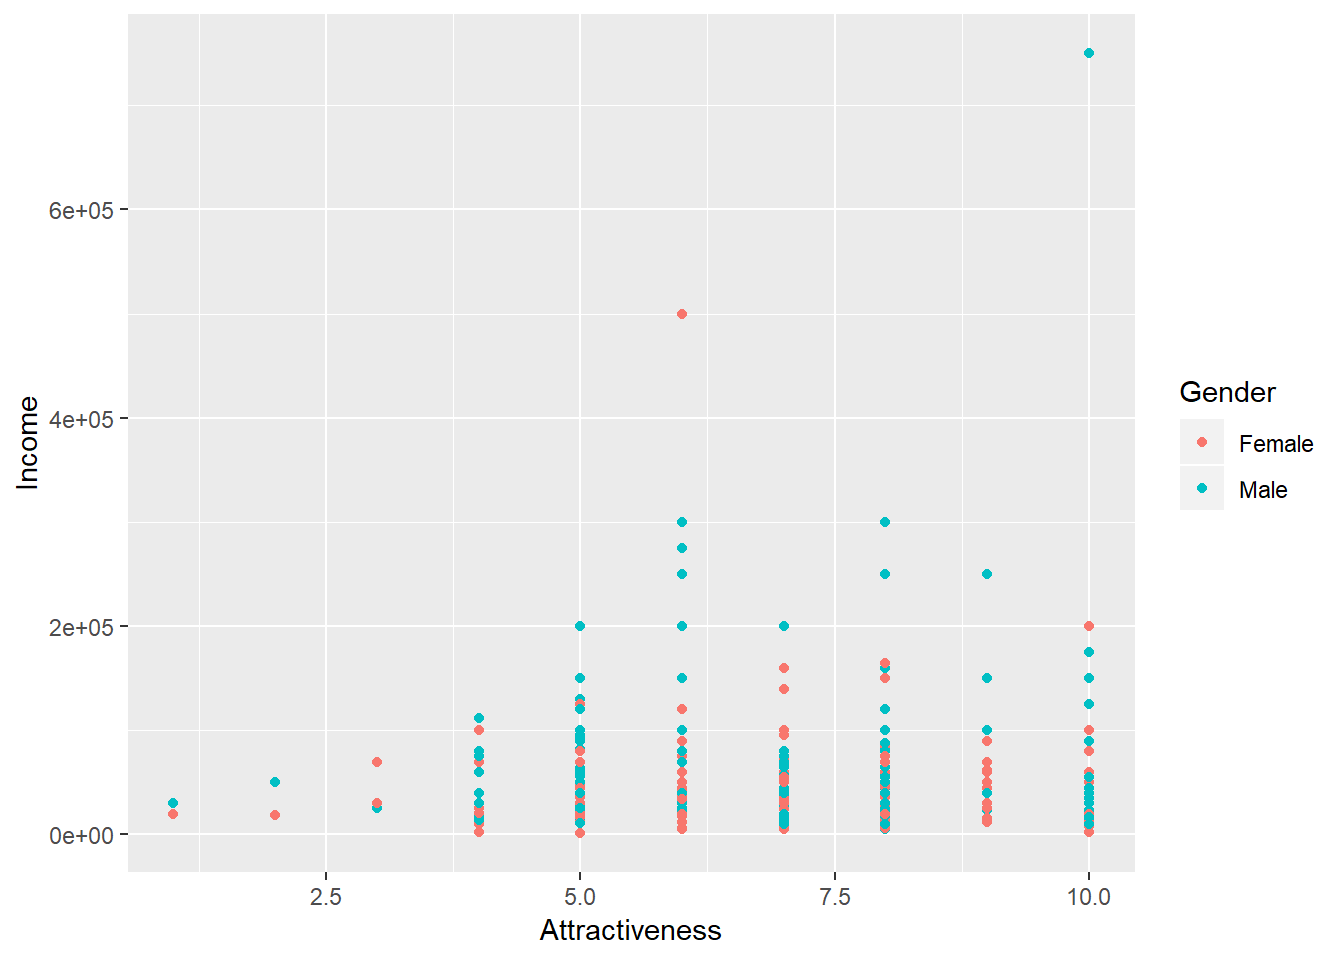
\includegraphics{Online_R_Course_files/figure-latex/unnamed-chunk-27-1.pdf}

\textbf{QUESTION: Before pressing run - predict what will happen in the following two chunks of code. After running - can you explain why?}

\textbf{A}

\begin{Shaded}
\begin{Highlighting}[]
\KeywordTok{ggplot}\NormalTok{(}\DataTypeTok{data =}\NormalTok{ Pulse,  }\KeywordTok{aes}\NormalTok{(}\DataTypeTok{x =}\NormalTok{ Attractiveness, }\DataTypeTok{y =}\NormalTok{ Income, }\DataTypeTok{colour=}\StringTok{"purple"}\NormalTok{)) }\OperatorTok{+}\StringTok{ }
\StringTok{  }\KeywordTok{geom_point}\NormalTok{()}
\end{Highlighting}
\end{Shaded}

\textbf{B}

\begin{Shaded}
\begin{Highlighting}[]
\KeywordTok{ggplot}\NormalTok{(}\DataTypeTok{data =}\NormalTok{ Pulse,  }\KeywordTok{aes}\NormalTok{(}\DataTypeTok{x =}\NormalTok{ Attractiveness, }\DataTypeTok{y =}\NormalTok{ Income)) }\OperatorTok{+}\StringTok{ }
\StringTok{  }\KeywordTok{geom_point}\NormalTok{(}\DataTypeTok{colour=}\NormalTok{Gender)}
\end{Highlighting}
\end{Shaded}

\hypertarget{more-geoms}{%
\section{More Geoms}\label{more-geoms}}

Let's go back to attractiveness. If instead we wanted a line plot we can simply replace \texttt{geom\_point()} with \texttt{geom\_line()}.

\begin{Shaded}
\begin{Highlighting}[]
\KeywordTok{ggplot}\NormalTok{(}\DataTypeTok{data =}\NormalTok{ Pulse,  }\KeywordTok{aes}\NormalTok{(}\DataTypeTok{x =}\NormalTok{ Attractiveness, }\DataTypeTok{y =}\NormalTok{ Income)) }\OperatorTok{+}\StringTok{ }
\StringTok{  }\KeywordTok{geom_line}\NormalTok{()}
\end{Highlighting}
\end{Shaded}

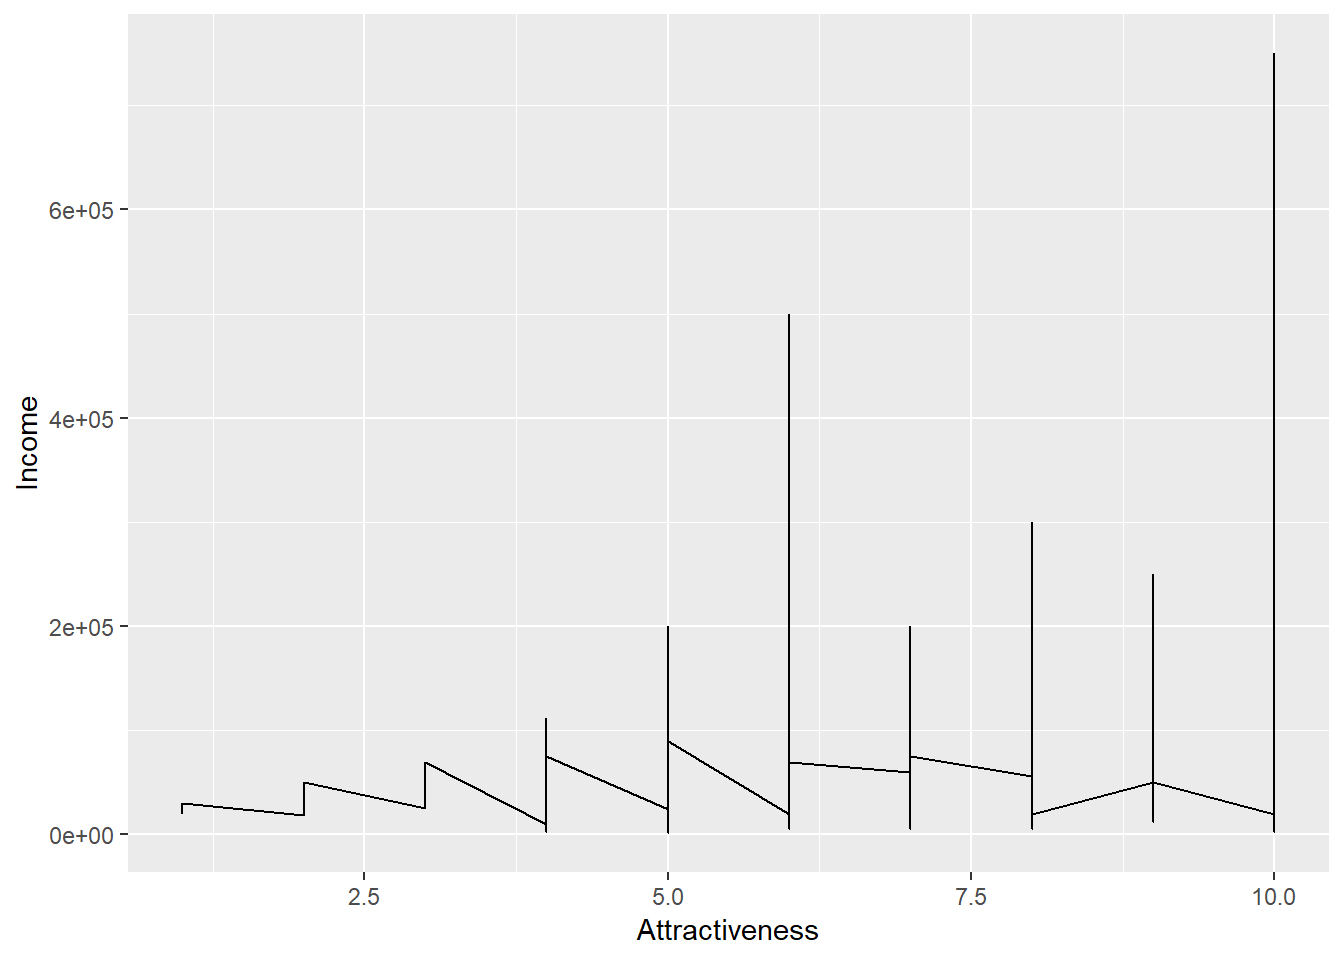
\includegraphics{Online_R_Course_files/figure-latex/unnamed-chunk-30-1.pdf}

This graph is not particularly helpful in conveying any useful information about our data. Just because something is possible, does not mean it is advisable.

A geom that may be more useful is \texttt{geom\_jitter()} - which would help us here because the attractiveness variable has a restricted set of values, so many points are being overlayed

\begin{Shaded}
\begin{Highlighting}[]
\KeywordTok{ggplot}\NormalTok{(}\DataTypeTok{data =}\NormalTok{ Pulse,  }\KeywordTok{aes}\NormalTok{(}\DataTypeTok{x =}\NormalTok{ Attractiveness, }\DataTypeTok{y =}\NormalTok{ Income)) }\OperatorTok{+}\StringTok{ }
\StringTok{  }\KeywordTok{geom_jitter}\NormalTok{()}
\end{Highlighting}
\end{Shaded}

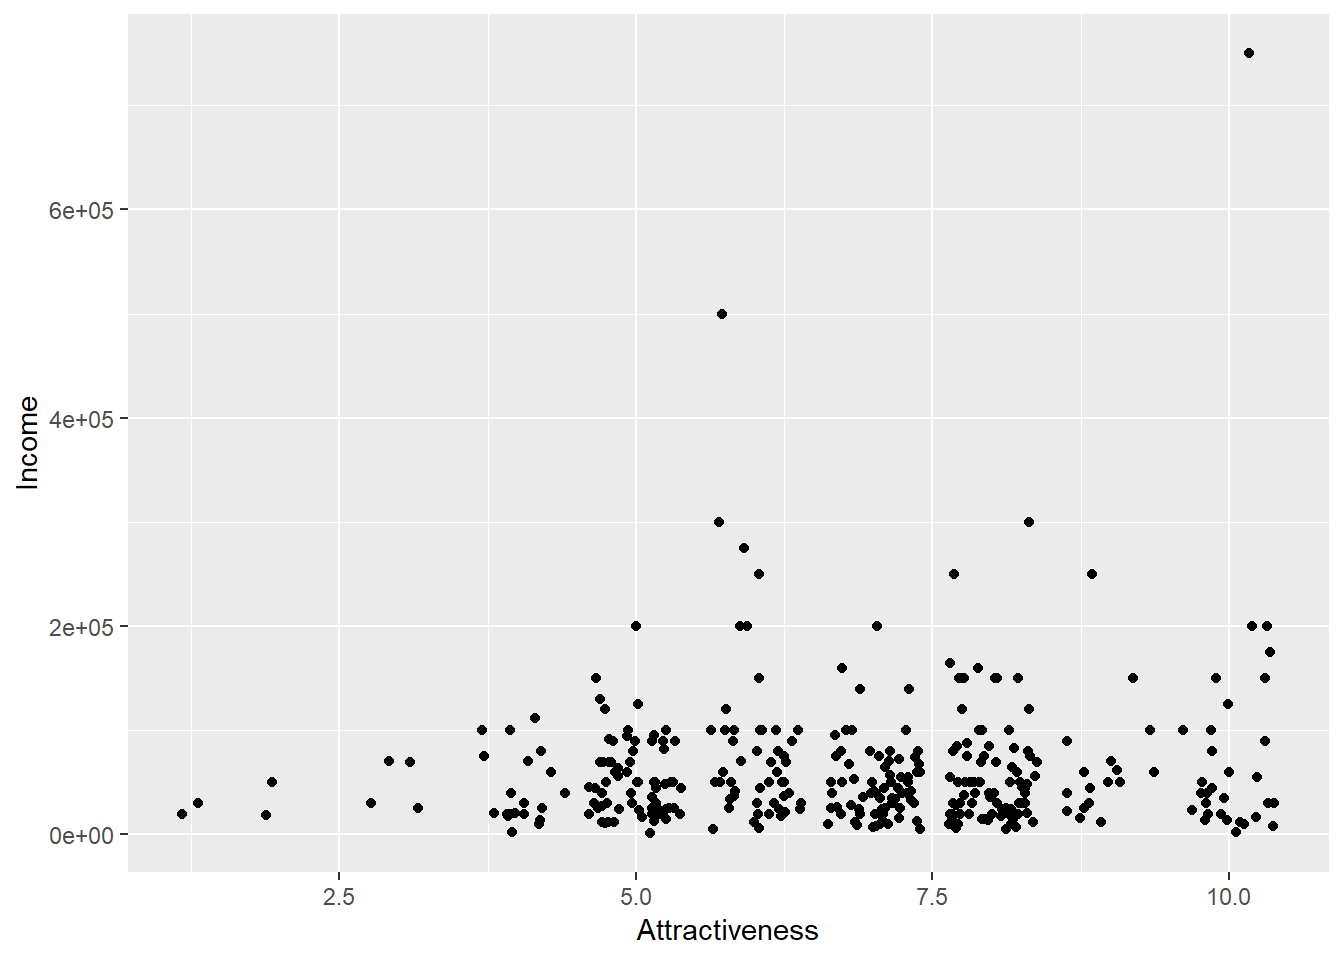
\includegraphics{Online_R_Course_files/figure-latex/unnamed-chunk-31-1.pdf}

The \texttt{geom\_****} functions all have various default options associated with them. For example, the size and colour of the points in \texttt{geom\_point()} or the amount of jitter associated with them in \texttt{geom\_jitter()}.

\textbf{QUESTION: Using the help menu for geom\_jitter can you modify the following code so that the amount of horizontal jitter is reduced and that there is no vertical jitter applied}

\begin{Shaded}
\begin{Highlighting}[]
\NormalTok{?geom_jitter}
\end{Highlighting}
\end{Shaded}

\begin{Shaded}
\begin{Highlighting}[]
\KeywordTok{ggplot}\NormalTok{(}\DataTypeTok{data =}\NormalTok{ Pulse,  }\KeywordTok{aes}\NormalTok{(}\DataTypeTok{x =}\NormalTok{ Attractiveness, }\DataTypeTok{y =}\NormalTok{ Income)) }\OperatorTok{+}\StringTok{ }
\StringTok{  }\KeywordTok{geom_jitter}\NormalTok{()}
\end{Highlighting}
\end{Shaded}

\hypertarget{scales}{%
\section{Scales}\label{scales}}

Income is a notoriously fickle variable. As we can see from the the table below there is a huge range in the values income takes, so when we have plotted Income against Attractiveness, most of our points are bunched up near the bottom.

We can show this by categorising our points in a table such as below;

\begin{tabular}{lr}
\toprule
Income & Freq\\
\midrule
\$1,000-\$9,999 & 13\\
\$10,000-\$99,999 & 278\\
\$100,000-\$999,999 & 59\\
\bottomrule
\end{tabular}

One solution is to apply a log scale for income. A log scale is when each tick mark of the graph represents an increase in the power.

\begin{center}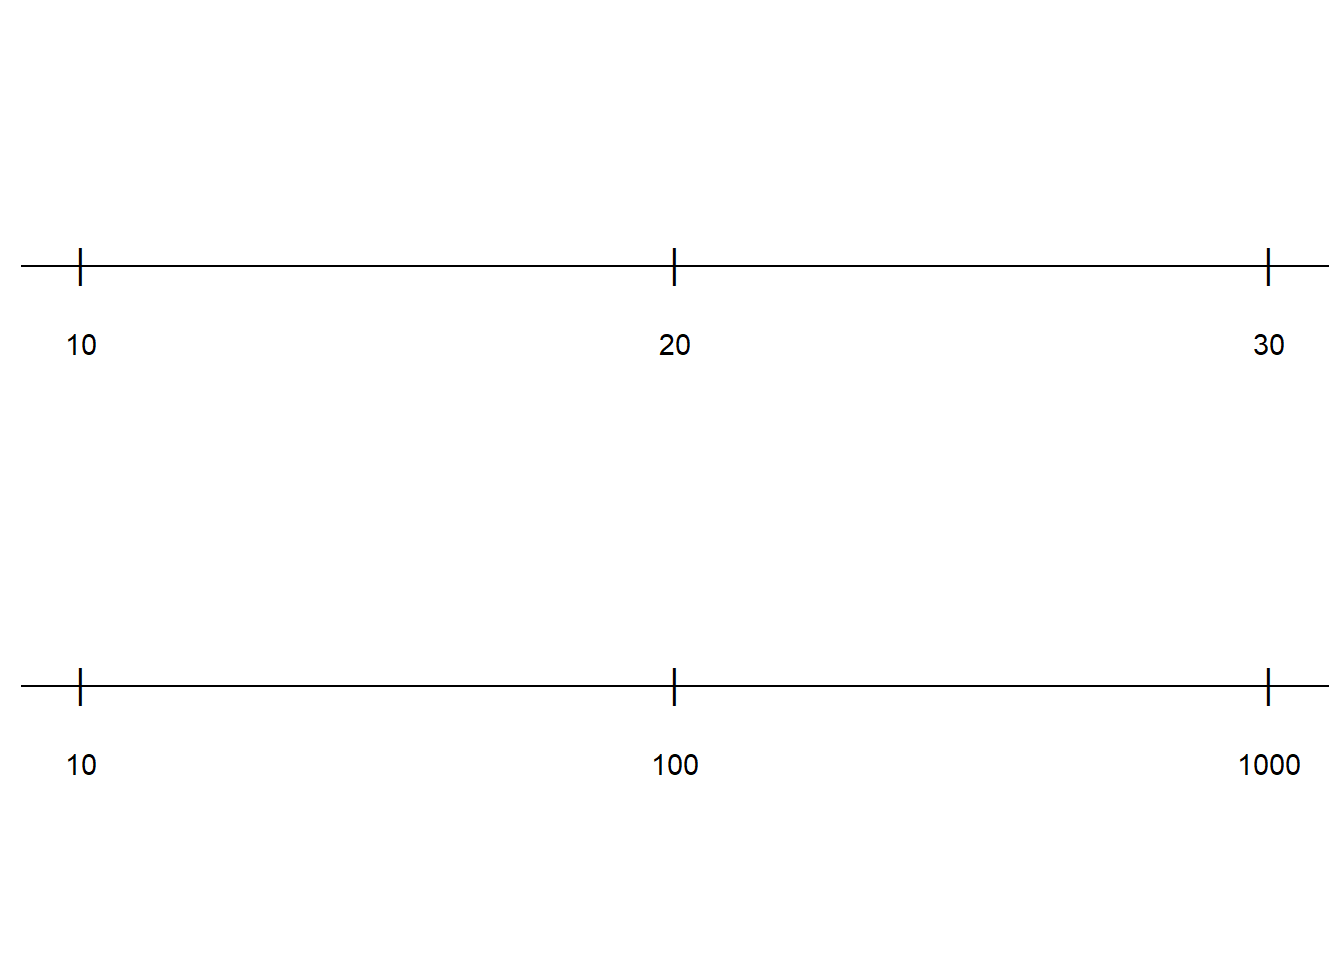
\includegraphics{Online_R_Course_files/figure-latex/unnamed-chunk-35-1} \end{center}

In the above example, the top line is increasing \emph{by} 10 whereas hde bottom line is increasing \emph{by powers of 10}. To apply this change of scale to our plot, we add the following code to our plot. \texttt{scale\_y\_log10()}

\begin{Shaded}
\begin{Highlighting}[]
\KeywordTok{ggplot}\NormalTok{(}\DataTypeTok{data =}\NormalTok{ Pulse,  }\KeywordTok{aes}\NormalTok{(}\DataTypeTok{x =}\NormalTok{ Attractiveness, }\DataTypeTok{y =}\NormalTok{ Income)) }\OperatorTok{+}\StringTok{ }
\StringTok{  }\KeywordTok{geom_jitter}\NormalTok{(}\DataTypeTok{width=}\FloatTok{0.25}\NormalTok{,}\DataTypeTok{height=}\DecValTok{0}\NormalTok{)}\OperatorTok{+}
\StringTok{    }\KeywordTok{scale_y_log10}\NormalTok{()}
\end{Highlighting}
\end{Shaded}

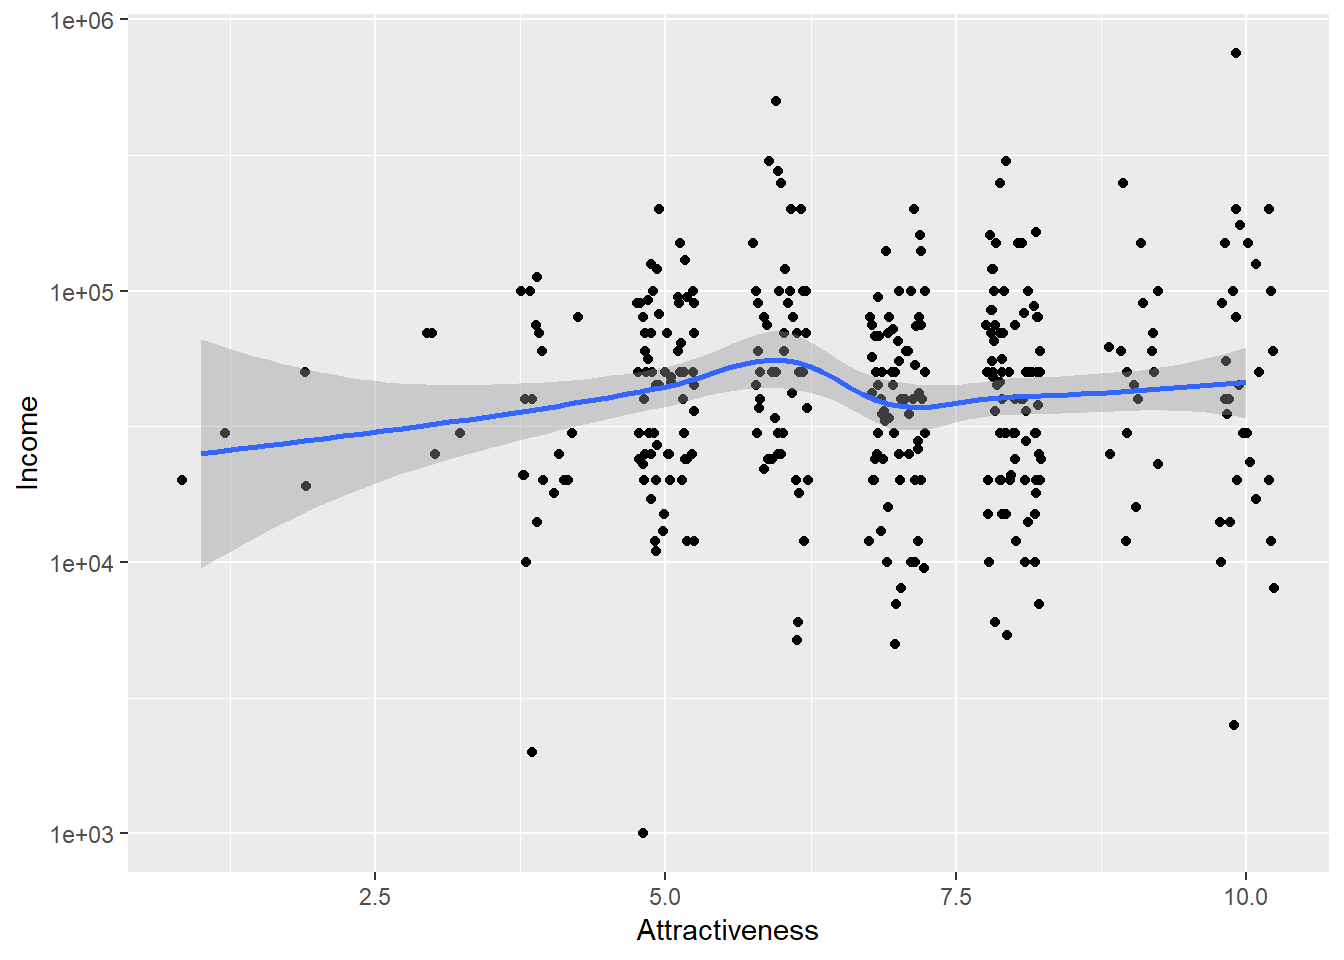
\includegraphics{Online_R_Course_files/figure-latex/unnamed-chunk-36-1.pdf}

\hypertarget{layering}{%
\section{Layering}\label{layering}}

ggplot2 graphs can have more than one layer. We may want to produce a line plot with the points shown on top. In ggplots we can simply add more layers to a graph by using \texttt{+}. Layers are added sequentially so the final layer in the code will be plotted over the existing layers. We might want to add a trend line onto our plot to show the increasing trend of income with attractiveness (or the increasing arrogance of wealth?)

\begin{Shaded}
\begin{Highlighting}[]
\KeywordTok{ggplot}\NormalTok{(}\DataTypeTok{data =}\NormalTok{ Pulse,  }\KeywordTok{aes}\NormalTok{(}\DataTypeTok{x =}\NormalTok{ Attractiveness, }\DataTypeTok{y =}\NormalTok{ Income)) }\OperatorTok{+}\StringTok{ }
\StringTok{  }\KeywordTok{geom_jitter}\NormalTok{(}\DataTypeTok{width=}\FloatTok{0.25}\NormalTok{,}\DataTypeTok{height=}\DecValTok{0}\NormalTok{)}\OperatorTok{+}
\StringTok{    }\KeywordTok{scale_y_log10}\NormalTok{()}\OperatorTok{+}
\StringTok{      }\KeywordTok{geom_smooth}\NormalTok{()}
\end{Highlighting}
\end{Shaded}

\begin{verbatim}
## `geom_smooth()` using method = 'loess' and formula 'y ~ x'
\end{verbatim}

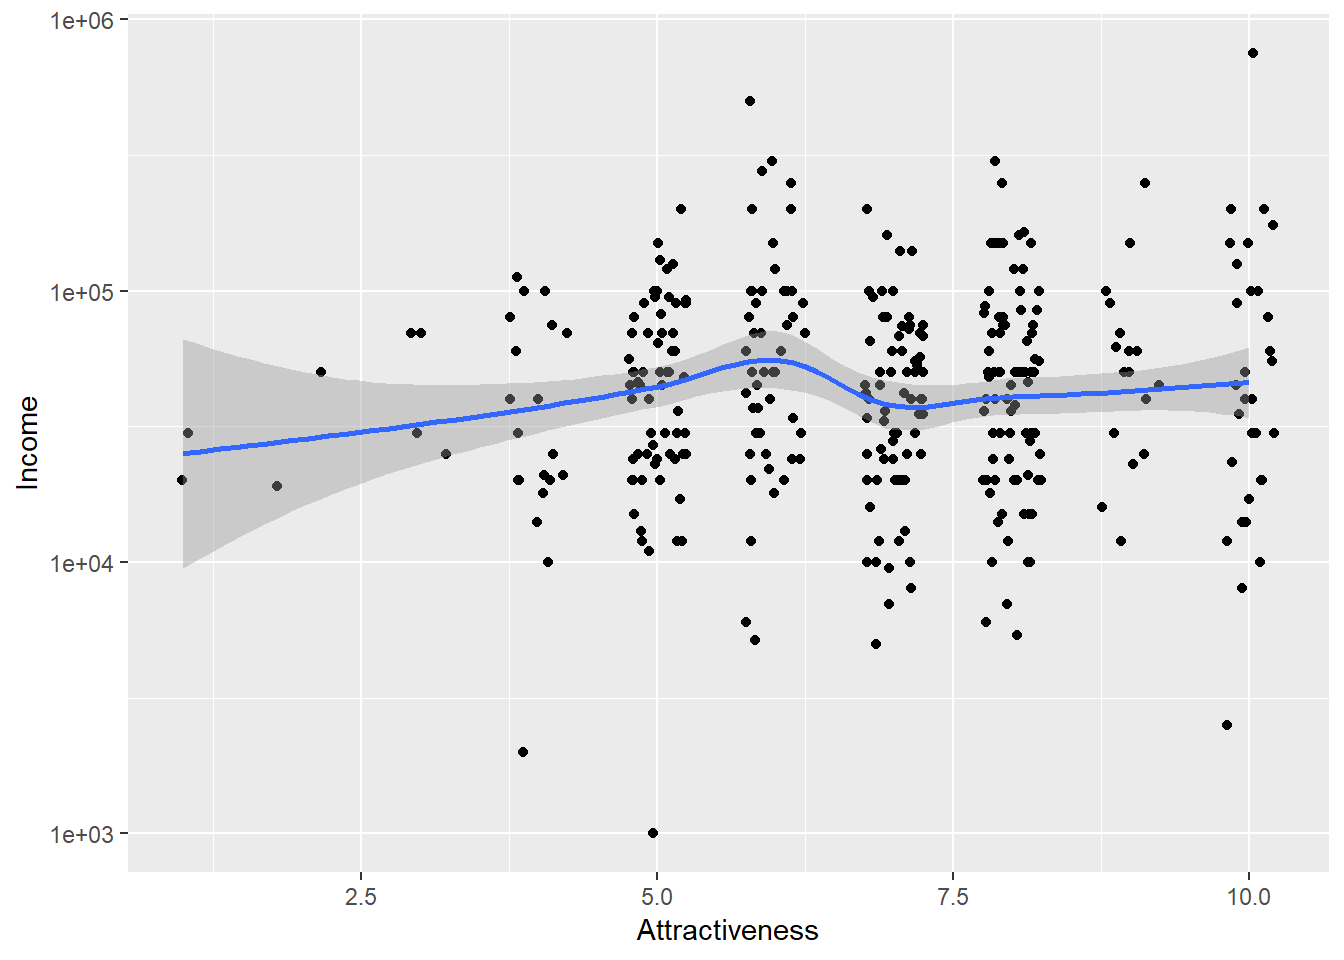
\includegraphics{Online_R_Course_files/figure-latex/unnamed-chunk-37-1.pdf}

\hypertarget{more-geoms-1}{%
\section{More geoms}\label{more-geoms-1}}

Bar charts are a popular (and horrifically misused way of presenting results). Let's look at a bar chart of number respondents by political affiliation. We have to think a little bit about how this will be presented - consider how a bar chart works. What goes on the x axis and what goes on the y axis?

\begin{Shaded}
\begin{Highlighting}[]
\KeywordTok{ggplot}\NormalTok{(}\DataTypeTok{data =}\NormalTok{ Pulse,  }\KeywordTok{aes}\NormalTok{(}\DataTypeTok{x =}\NormalTok{ PoliticalParty))}\OperatorTok{+}
\StringTok{  }\KeywordTok{geom_bar}\NormalTok{()}
\end{Highlighting}
\end{Shaded}

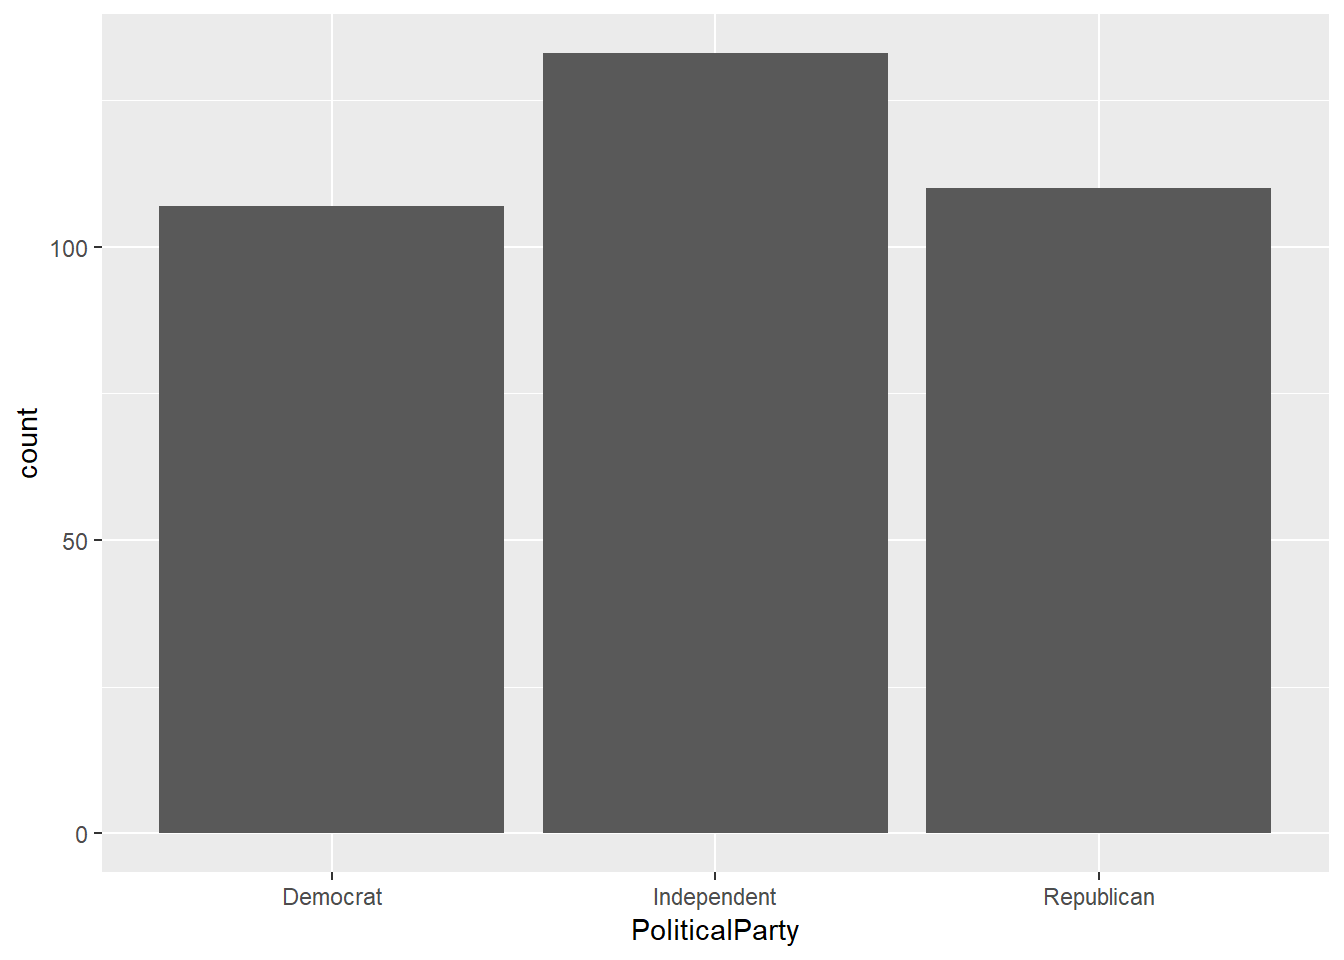
\includegraphics{Online_R_Course_files/figure-latex/unnamed-chunk-38-1.pdf}

To bring in a second variable then you can map this to the colour or fill aesthetics.

\begin{Shaded}
\begin{Highlighting}[]
\KeywordTok{ggplot}\NormalTok{(}\DataTypeTok{data =}\NormalTok{ Pulse,  }\KeywordTok{aes}\NormalTok{(}\DataTypeTok{x =}\NormalTok{ PoliticalParty,}\DataTypeTok{fill=}\NormalTok{Gender))}\OperatorTok{+}
\StringTok{  }\KeywordTok{geom_bar}\NormalTok{(}\DataTypeTok{colour=}\StringTok{"black"}\NormalTok{)}
\end{Highlighting}
\end{Shaded}

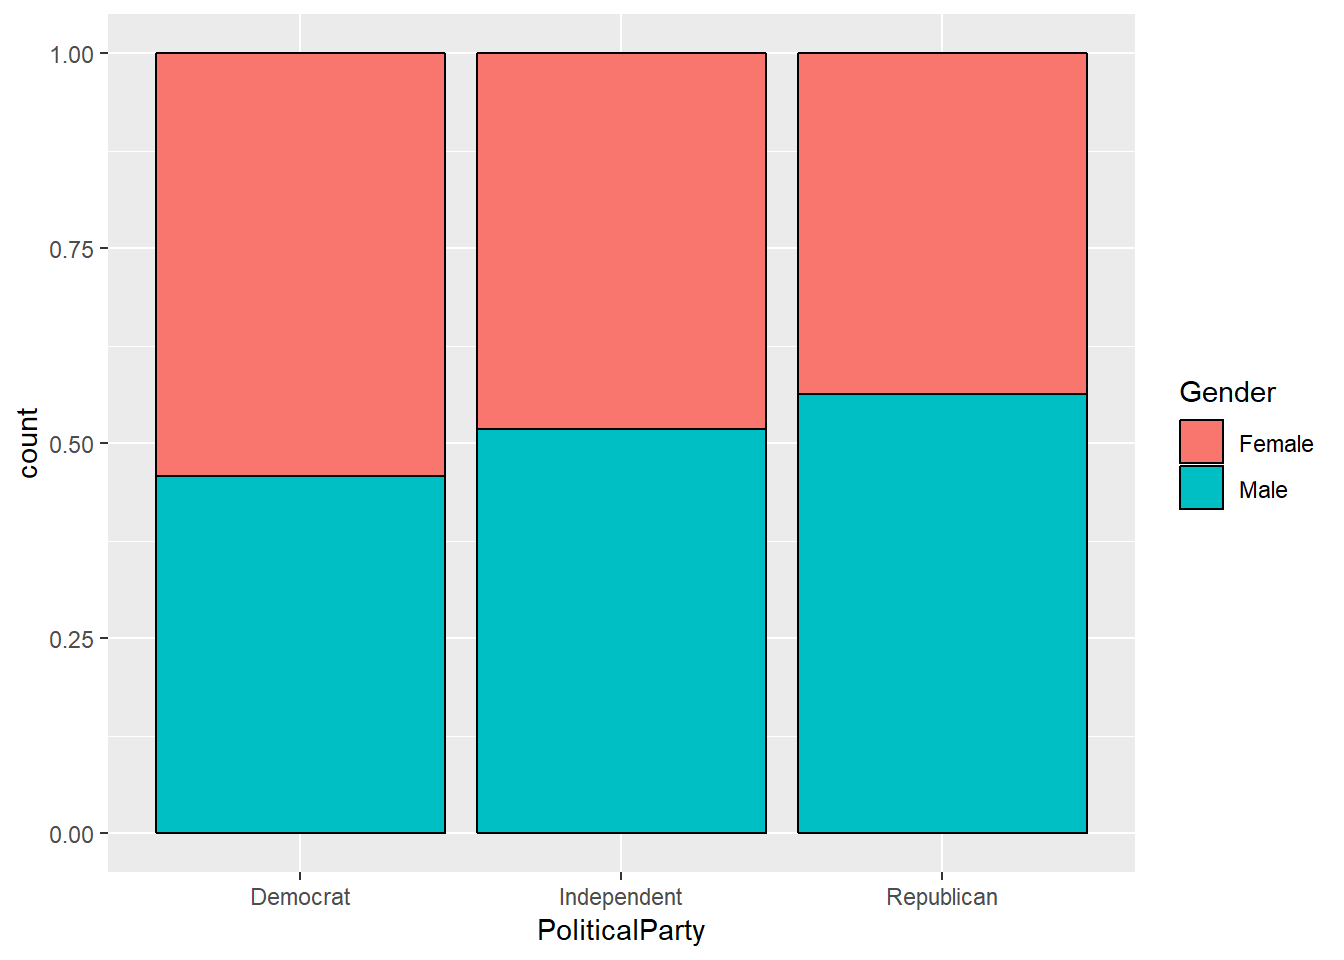
\includegraphics{Online_R_Course_files/figure-latex/unnamed-chunk-39-1.pdf}

It's hard to make the direct comparison across our three parties - so we can convert to proportions use position=``fill''

\begin{Shaded}
\begin{Highlighting}[]
\KeywordTok{ggplot}\NormalTok{(}\DataTypeTok{data =}\NormalTok{ Pulse,  }\KeywordTok{aes}\NormalTok{(}\DataTypeTok{x =}\NormalTok{ PoliticalParty,}\DataTypeTok{fill=}\NormalTok{Gender))}\OperatorTok{+}
\StringTok{  }\KeywordTok{geom_bar}\NormalTok{(}\DataTypeTok{colour=}\StringTok{"black"}\NormalTok{,}\DataTypeTok{position=}\StringTok{"fill"}\NormalTok{)}
\end{Highlighting}
\end{Shaded}

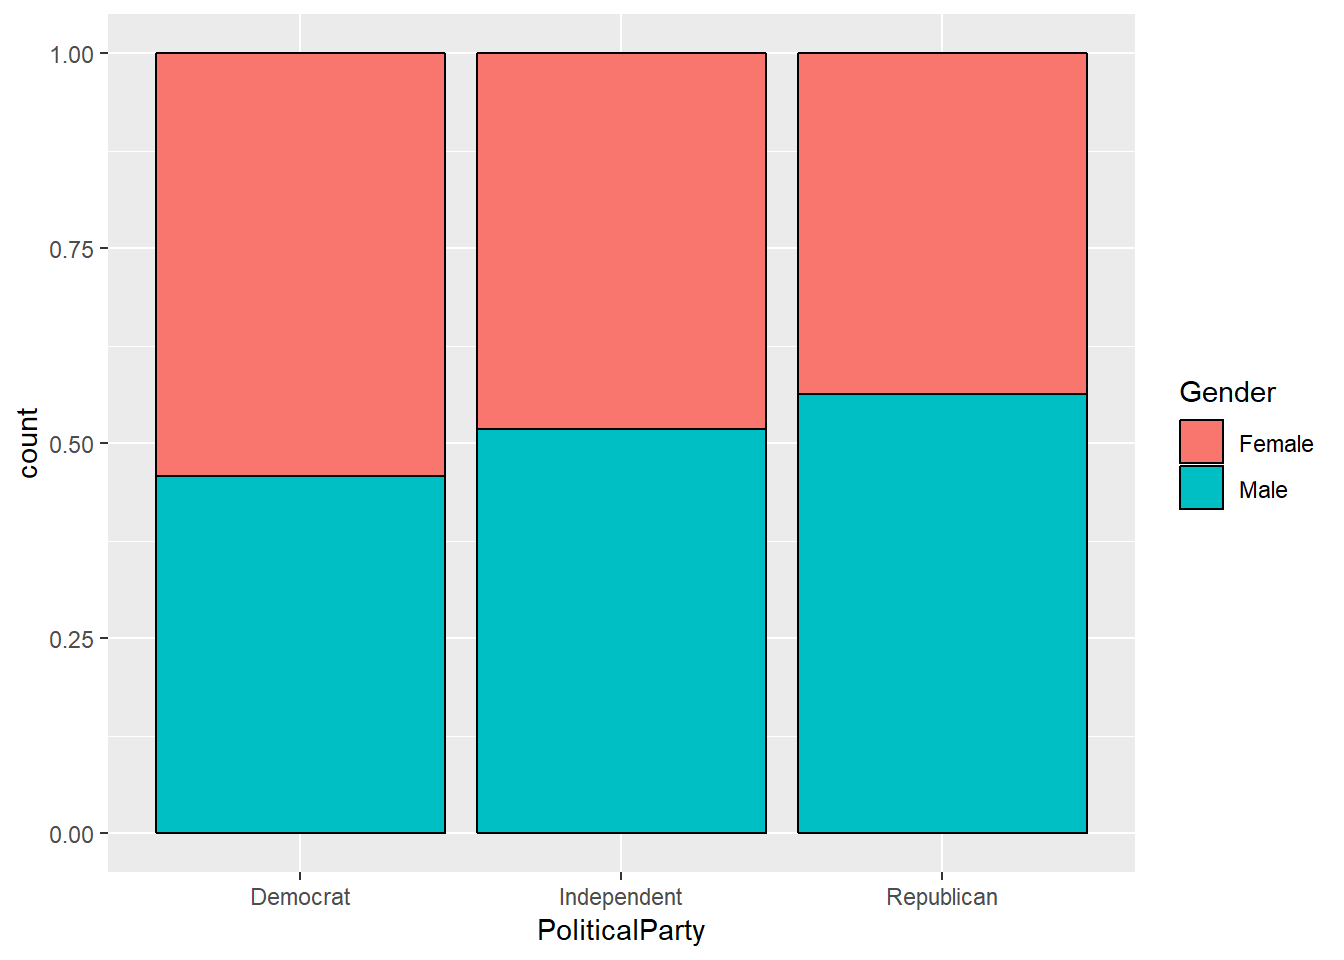
\includegraphics{Online_R_Course_files/figure-latex/unnamed-chunk-40-1.pdf}

\textbf{QUESTION: Try removing \texttt{colour="black"} and describe the difference}

\textbf{QUESTION: Make an (informative) bar chart of level of support for Donald Trump by Gender}

\begin{Shaded}
\begin{Highlighting}[]
\KeywordTok{ggplot}\NormalTok{(}\DataTypeTok{data =}\NormalTok{ Pulse,  }\KeywordTok{aes}\NormalTok{())}\OperatorTok{+}
\StringTok{  }\KeywordTok{geom_bar}\NormalTok{()}
\end{Highlighting}
\end{Shaded}

\hypertarget{comparing-attractiveness-across-gender}{%
\section{Comparing attractiveness across gender}\label{comparing-attractiveness-across-gender}}

How can we compare attractiveness across gender in a better way than colouring the points? There are lots of other geoms which might help here. We could produce a boxplot to summarise the level of attractiveness by gender.

\textbf{QUESTION: Find the geom function for a boxplot and complete the code below to produce a boxplot of attractiveness by gender}

\begin{Shaded}
\begin{Highlighting}[]
\KeywordTok{ggplot}\NormalTok{(}\DataTypeTok{data =}\NormalTok{ Pulse,  }\KeywordTok{aes}\NormalTok{(}\DataTypeTok{x =}\NormalTok{ ?????, }\DataTypeTok{y =}\NormalTok{ ?????))}\OperatorTok{+}
\StringTok{  }\NormalTok{geom_?????()}
\end{Highlighting}
\end{Shaded}

The labelling on the y axis is kind of ugly here. Not many people work in base 2.5; but R makes some assumptions on how to label the plots so that it can fit in an `optimal' number of labels. Let's use scale\_y\_continuous() to modify this so that all points between 1 and 10 are labelled:

\begin{Shaded}
\begin{Highlighting}[]
\KeywordTok{ggplot}\NormalTok{(}\DataTypeTok{data =}\NormalTok{ Pulse,  }\KeywordTok{aes}\NormalTok{(}\DataTypeTok{x =}\NormalTok{ ?????, }\DataTypeTok{y =}\NormalTok{ ?????))}\OperatorTok{+}
\StringTok{  }\NormalTok{geom_?????()}\OperatorTok{+}
\StringTok{    }\KeywordTok{scale_y_continuous}\NormalTok{(}\DataTypeTok{breaks=}\DecValTok{1}\OperatorTok{:}\DecValTok{10}\NormalTok{)}
\end{Highlighting}
\end{Shaded}

Violin plots are also a really nice way of summarising data in a similar way to boxplots
\#\#Do we want to remove the answer to the earlier questions?

\begin{Shaded}
\begin{Highlighting}[]
\KeywordTok{ggplot}\NormalTok{(}\DataTypeTok{data =}\NormalTok{ Pulse,  }\KeywordTok{aes}\NormalTok{(}\DataTypeTok{x =}\NormalTok{ Gender, }\DataTypeTok{y =}\NormalTok{ Attractiveness))}\OperatorTok{+}
\StringTok{  }\KeywordTok{geom_violin}\NormalTok{()}\OperatorTok{+}
\StringTok{    }\KeywordTok{scale_y_continuous}\NormalTok{(}\DataTypeTok{breaks=}\DecValTok{1}\OperatorTok{:}\DecValTok{10}\NormalTok{)}
\end{Highlighting}
\end{Shaded}

\textbf{QUESTION: Modify the following code so that the violins are shaded in different colours for men and women. (Hint: You might need to consult the help menu to look for a new aesthetic we haven't mentioned yet}

\begin{Shaded}
\begin{Highlighting}[]
\KeywordTok{ggplot}\NormalTok{(}\DataTypeTok{data =}\NormalTok{ Pulse,  }\KeywordTok{aes}\NormalTok{(}\DataTypeTok{x =}\NormalTok{ Gender, }\DataTypeTok{y =}\NormalTok{ Attractiveness))}\OperatorTok{+}
\StringTok{  }\KeywordTok{geom_violin}\NormalTok{()}\OperatorTok{+}
\StringTok{    }\KeywordTok{scale_y_continuous}\NormalTok{(}\DataTypeTok{breaks=}\DecValTok{1}\OperatorTok{:}\DecValTok{10}\NormalTok{)}
\end{Highlighting}
\end{Shaded}

\hypertarget{splitting-plots-using-facets}{%
\section{Splitting plots using Facets}\label{splitting-plots-using-facets}}

We've seen how to add variables to a plot using aesthetics. Another way, particularly useful for categorical variables, is to split your plot into facets, which are subplots that each display one subset of the data.

\begin{Shaded}
\begin{Highlighting}[]
\KeywordTok{ggplot}\NormalTok{(}\DataTypeTok{data =}\NormalTok{ Pulse,  }\KeywordTok{aes}\NormalTok{(}\DataTypeTok{x =}\NormalTok{ Gender, }\DataTypeTok{y =}\NormalTok{ Attractiveness,}\DataTypeTok{fill=}\NormalTok{Gender))}\OperatorTok{+}
\StringTok{  }\KeywordTok{geom_violin}\NormalTok{()}\OperatorTok{+}
\StringTok{    }\KeywordTok{scale_y_continuous}\NormalTok{(}\DataTypeTok{breaks=}\DecValTok{1}\OperatorTok{:}\DecValTok{10}\NormalTok{) }\OperatorTok{+}
\StringTok{      }\KeywordTok{facet_wrap}\NormalTok{(}\OperatorTok{~}\NormalTok{PoliticalParty)}
\end{Highlighting}
\end{Shaded}

Be careful not to miss the \textasciitilde{} before country. This is used to define a formula which can have something on both sides of \textasciitilde{} in general. It's used in many R function, and you'll see this more later in modelling.

\hypertarget{themes-and-labels}{%
\section{Themes and labels}\label{themes-and-labels}}

Themes refers to the non data elements of your plot. ggplot2 has a huge number of theme options that allows you to control almost every aspect of your plot which becomes important when you want to present or publish your graphs.

The labs() function allows us to label any of our variables and create a title. We only need to change options that we are unhappy with.

\begin{Shaded}
\begin{Highlighting}[]
\KeywordTok{ggplot}\NormalTok{(}\DataTypeTok{data =}\NormalTok{ Pulse,  }\KeywordTok{aes}\NormalTok{(}\DataTypeTok{x =}\NormalTok{ Gender, }\DataTypeTok{y =}\NormalTok{ Attractiveness,}\DataTypeTok{fill=}\NormalTok{Gender))}\OperatorTok{+}
\StringTok{  }\KeywordTok{geom_violin}\NormalTok{()}\OperatorTok{+}
\StringTok{    }\KeywordTok{scale_y_continuous}\NormalTok{(}\DataTypeTok{breaks=}\DecValTok{1}\OperatorTok{:}\DecValTok{10}\NormalTok{) }\OperatorTok{+}
\StringTok{     }\KeywordTok{facet_wrap}\NormalTok{(}\OperatorTok{~}\NormalTok{PoliticalParty)}\OperatorTok{+}
\StringTok{      }\KeywordTok{labs}\NormalTok{(}\DataTypeTok{x=}\StringTok{"Gender"}\NormalTok{,}\DataTypeTok{y =} \StringTok{"Perceived Physical Attractivess"}\NormalTok{,}\DataTypeTok{colour=}\StringTok{"Gender (again)"}\NormalTok{,}\DataTypeTok{title =} \StringTok{"Violin Plots of Physical Attractiveness by Gender and Political   Affiliation"}\NormalTok{)}
\end{Highlighting}
\end{Shaded}

theme() allows us to modify the size, font, face of labels and the appearance of many other attributes of the plot which do not depend on the data.

\begin{Shaded}
\begin{Highlighting}[]
\NormalTok{?theme}
\end{Highlighting}
\end{Shaded}

You will see a a huge number of arguments. You don't need to learn them all, but you can find out about them on that page. Let's say we want to edit the text on the x axis, which is the axis.text.x argument. We can modify different properties of the text through the element\_text() function. Let's look at that.

\begin{Shaded}
\begin{Highlighting}[]
\NormalTok{?element_text}
\end{Highlighting}
\end{Shaded}

We can see it has arguments such as family (for font), colour, size and angle etc.

\textbf{QUESTION: Investigate the element\_text() function to make the text labels on the x axis large and bold}

\begin{Shaded}
\begin{Highlighting}[]
\KeywordTok{ggplot}\NormalTok{(}\DataTypeTok{data =}\NormalTok{ Pulse,  }\KeywordTok{aes}\NormalTok{(}\DataTypeTok{x =}\NormalTok{ Gender, }\DataTypeTok{y =}\NormalTok{ Attractiveness,}\DataTypeTok{fill=}\NormalTok{Gender))}\OperatorTok{+}
\StringTok{  }\KeywordTok{geom_violin}\NormalTok{()}\OperatorTok{+}
\StringTok{    }\KeywordTok{scale_y_continuous}\NormalTok{(}\DataTypeTok{breaks=}\DecValTok{1}\OperatorTok{:}\DecValTok{10}\NormalTok{) }\OperatorTok{+}
\StringTok{     }\KeywordTok{facet_wrap}\NormalTok{(}\OperatorTok{~}\NormalTok{PoliticalParty)}\OperatorTok{+}
\StringTok{      }\KeywordTok{labs}\NormalTok{(}\DataTypeTok{x=}\StringTok{"Gender"}\NormalTok{,}\DataTypeTok{y =} \StringTok{"Perceived Physical Attractivess"}\NormalTok{,}\DataTypeTok{colour=}\StringTok{"Gender (again)"}\NormalTok{,}\DataTypeTok{title =} \StringTok{"Violin Plots of Physical Attractiveness by Gender and Political   Affiliation"}\NormalTok{) }\OperatorTok{+}\StringTok{ }
\StringTok{       }\KeywordTok{theme}\NormalTok{(}\DataTypeTok{axis.text.x =} \KeywordTok{element_text}\NormalTok{(????))}
\end{Highlighting}
\end{Shaded}

\hypertarget{recap-exercises}{%
\section{Recap Exercises}\label{recap-exercises}}

\textbf{Fix the error(s) in this code to produce a boxplot of attractiveness by age group}

\begin{Shaded}
\begin{Highlighting}[]
\KeywordTok{ggplot}\NormalTok{(}\DataTypeTok{data =}\NormalTok{ Pulse,  }\KeywordTok{aes}\NormalTok{(}\DataTypeTok{x =}\NormalTok{ agegroup, }\DataTypeTok{y =}\NormalTok{ attractiveness))}\OperatorTok{+}
\StringTok{  }\KeywordTok{geom_boxplot}\NormalTok{()}
\end{Highlighting}
\end{Shaded}

\textbf{Fill in the blanks to produce a scatter plot of attractiveness (y axis) by age (x axis)}

\begin{Shaded}
\begin{Highlighting}[]
\KeywordTok{ggplot}\NormalTok{(}\DataTypeTok{data =}\NormalTok{ Pulse,  }\KeywordTok{aes}\NormalTok{(??????))}\OperatorTok{+}
\StringTok{  }\NormalTok{geom_????()}
\end{Highlighting}
\end{Shaded}

\textbf{Continuing the previous example, modify the scale on the y axis to show every number between 1 and 10 and the x axis to show every 20 years}

\begin{Shaded}
\begin{Highlighting}[]
\KeywordTok{ggplot}\NormalTok{(}\DataTypeTok{data =}\NormalTok{ Pulse,  }\KeywordTok{aes}\NormalTok{(??????))}\OperatorTok{+}
\StringTok{  }\NormalTok{geom_????()}
\end{Highlighting}
\end{Shaded}

\textbf{Produce boxplots of income by gender, with seperate panels for each age group. Use some colours, set a log axis for income, and add sensible titles and labels }

\begin{Shaded}
\begin{Highlighting}[]
\KeywordTok{ggplot}\NormalTok{(}\DataTypeTok{data =}\NormalTok{ Pulse, ...}
\end{Highlighting}
\end{Shaded}

\textbf{Produce a graph to investigate the is a relationship between income and education; and the extent to which this varies by gender.}

\hypertarget{data-manipulation-with-dplyr}{%
\chapter{Data Manipulation with dplyr}\label{data-manipulation-with-dplyr}}

The previous chapter introduced \texttt{ggplot2} which expanded our Base-R vocabulary to help us visualise our data easier.

Now, what if our dataset isn't organised quite the way we want it to create a plot? Maybe it's missing a column we need? Maybe missing values are encoded stragangely? Perhaps we need to standarise the units in a column?

We can use another package to solve these problems - \texttt{dplyr}! \citep{R-dplyr}

Like \texttt{ggplot2}, it adds more words to our R vocabulary and is focused on organising your data. \texttt{dplyr} is short for ``data frame plier''. Data frames are an object type in \texttt{R} but we don't think it is useful to discuss object types in this tutorial. \texttt{data\ frames} are essentially tables that stores your data in R.

\hypertarget{set-up-for-session}{%
\section{Set Up for Session}\label{set-up-for-session}}

Similarly to the previous chapter, it is assumed you have R Studio running and have installed \texttt{ggplot2} and \texttt{dplyr}. If not, run the following code;

\begin{Shaded}
\begin{Highlighting}[]
\KeywordTok{install.packages}\NormalTok{(}\KeywordTok{c}\NormalTok{(}\StringTok{"ggplot2"}\NormalTok{,}\StringTok{"dplyr"}\NormalTok{))}
\end{Highlighting}
\end{Shaded}

We begin by loading \texttt{dplyr} and \texttt{ggplot2}.

\begin{Shaded}
\begin{Highlighting}[]
\KeywordTok{library}\NormalTok{(dplyr)}
\KeywordTok{library}\NormalTok{(ggplot2)}
\end{Highlighting}
\end{Shaded}

When you load \texttt{dplyr} you will get a warning message;

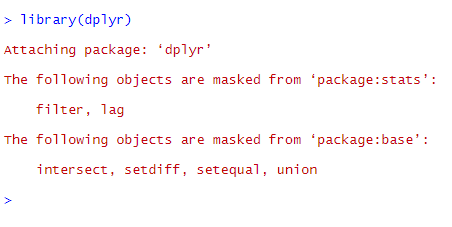
\includegraphics[width=6.28in]{Images/dplyrerror}

\textbf{Don't worry!}.

What it is saying is that \texttt{dplyr} has a few functions with the same name as built-in functions, so it will now use the ones from \texttt{dplyr} by default when these are called.

\textbf{QUESTION: Can you match the interpretation of the error with what is written in the error message? Why do you think they haved used the phrase `masked'?}

\begin{Shaded}
\begin{Highlighting}[]
\KeywordTok{library}\NormalTok{(dplyr)}
\KeywordTok{library}\NormalTok{(ggplot2)}
\end{Highlighting}
\end{Shaded}

Let's start by loading the miniIMDB dataset. This process is that same as described in the \protect\hyperlink{ggplot2_setting_up}{previous chapter} but loading \texttt{04-miniImdb.RData} instead of \texttt{03\ Pulse.RData}.

\hypertarget{description-of-datasets-being-used}{%
\section{Description of Datasets Being Used}\label{description-of-datasets-being-used}}

The ``imdb'' dataset has been built from the subsets of the Internet Movie Database made available for non-commercial purposes by the IMDb team: \citet{imdb}

It contains the following informations for all the entries having more than 500 votes, that are not of type ``tvEpisodes'' and for which information about year of release, running time and director(s) was available at the time of extraction (24/10/2018):

\begin{longtable}[]{@{}ll@{}}
\toprule
\begin{minipage}[b]{0.12\columnwidth}\raggedright
Variable\strut
\end{minipage} & \begin{minipage}[b]{0.82\columnwidth}\raggedright
Meaning\strut
\end{minipage}\tabularnewline
\midrule
\endhead
\begin{minipage}[t]{0.12\columnwidth}\raggedright
title\strut
\end{minipage} & \begin{minipage}[t]{0.82\columnwidth}\raggedright
the popular title of the entry\strut
\end{minipage}\tabularnewline
\begin{minipage}[t]{0.12\columnwidth}\raggedright
type\strut
\end{minipage} & \begin{minipage}[t]{0.82\columnwidth}\raggedright
type of the entry: movie short, tvMiniSeries, tvMovie, tvSeries, tvShort, tvSpecial, video or videoGame\strut
\end{minipage}\tabularnewline
\begin{minipage}[t]{0.12\columnwidth}\raggedright
year\strut
\end{minipage} & \begin{minipage}[t]{0.82\columnwidth}\raggedright
the year of release or start of release for series\strut
\end{minipage}\tabularnewline
\begin{minipage}[t]{0.12\columnwidth}\raggedright
length\strut
\end{minipage} & \begin{minipage}[t]{0.82\columnwidth}\raggedright
the duration of the running time in minutes\strut
\end{minipage}\tabularnewline
\begin{minipage}[t]{0.12\columnwidth}\raggedright
director\strut
\end{minipage} & \begin{minipage}[t]{0.82\columnwidth}\raggedright
the director (or director appearing first in the list of directors)\strut
\end{minipage}\tabularnewline
\begin{minipage}[t]{0.12\columnwidth}\raggedright
birthYear\strut
\end{minipage} & \begin{minipage}[t]{0.82\columnwidth}\raggedright
year of birth of director\strut
\end{minipage}\tabularnewline
\begin{minipage}[t]{0.12\columnwidth}\raggedright
NumVotes\strut
\end{minipage} & \begin{minipage}[t]{0.82\columnwidth}\raggedright
number of votes for the entry\strut
\end{minipage}\tabularnewline
\begin{minipage}[t]{0.12\columnwidth}\raggedright
averageRating\strut
\end{minipage} & \begin{minipage}[t]{0.82\columnwidth}\raggedright
IMDb's weighted average rating for the entry\strut
\end{minipage}\tabularnewline
\bottomrule
\end{longtable}

As well as a list of logical (TRUE/FALSE) columns qualifying the genre of the entry:

\begin{tabular}{c}
\toprule
Genres\\
\midrule
animation\\
action\\
adventure\\
comedy\\
documentary\\
\addlinespace
fantasy\\
romance\\
sci\_fi\\
thriller\\
\bottomrule
\end{tabular}

The ``miniImdb'' dataset is a small subset of ``imdb''. It contains the following 5 first variables of ``imdb'' for the titles that have received more than 1 million votes:

\begin{tabular}{c}
\toprule
miniImdb\\
\midrule
title\\
type\\
year\\
length\\
numVotes\\
\bottomrule
\end{tabular}

We will start by using the miniImdb dataset but we will later move to the full imdb dataset when we get more familiar with data manipulation.

\hypertarget{slicing-filter-and-select}{%
\section{Slicing, Filter and Select}\label{slicing-filter-and-select}}

We can use square brackets as a `quick' way to get subsets of datasets (also called slicing) based on position;

\texttt{DATASETNAME{[}ROW\ NUMBERS,COLUMN\ NUMBERS{]}}

\begin{Shaded}
\begin{Highlighting}[]
\NormalTok{miniImdb[}\DecValTok{1}\NormalTok{,]}
\end{Highlighting}
\end{Shaded}

\begin{verbatim}
## # A tibble: 1 x 5
##   title         type   year length numVotes
##   <chr>         <fct> <dbl>  <dbl>    <int>
## 1 The Godfather movie  1972    175  1374861
\end{verbatim}

\begin{Shaded}
\begin{Highlighting}[]
\NormalTok{miniImdb[,}\DecValTok{1}\NormalTok{]}
\end{Highlighting}
\end{Shaded}

\begin{verbatim}
## # A tibble: 29 x 1
##    title                                            
##    <chr>                                            
##  1 The Godfather                                    
##  2 Star Wars: Episode IV - A New Hope               
##  3 Star Wars: Episode V - The Empire Strikes Back   
##  4 The Silence of the Lambs                         
##  5 Schindler's List                                 
##  6 Forrest Gump                                     
##  7 Pulp Fiction                                     
##  8 The Shawshank Redemption                         
##  9 Se7en                                            
## 10 The Lord of the Rings: The Fellowship of the Ring
## # ... with 19 more rows
\end{verbatim}

\begin{Shaded}
\begin{Highlighting}[]
\NormalTok{miniImdb[}\DecValTok{1}\OperatorTok{:}\DecValTok{5}\NormalTok{,}\DecValTok{1}\OperatorTok{:}\DecValTok{2}\NormalTok{]}
\end{Highlighting}
\end{Shaded}

\begin{verbatim}
## # A tibble: 5 x 2
##   title                                          type 
##   <chr>                                          <fct>
## 1 The Godfather                                  movie
## 2 Star Wars: Episode IV - A New Hope             movie
## 3 Star Wars: Episode V - The Empire Strikes Back movie
## 4 The Silence of the Lambs                       movie
## 5 Schindler's List                               movie
\end{verbatim}

But to get more useful subsets we would probably need to base these on characteristics or names rather than positions. We can use the \texttt{filter()} and \texttt{select()} functions for that from \texttt{dplyr}.

filter() helps you get the rows you are interested in

\begin{Shaded}
\begin{Highlighting}[]
\KeywordTok{filter}\NormalTok{(miniImdb, type}\OperatorTok{==}\StringTok{"tvSeries"}\NormalTok{)}
\end{Highlighting}
\end{Shaded}

\begin{Shaded}
\begin{Highlighting}[]
\KeywordTok{filter}\NormalTok{(miniImdb, year}\OperatorTok{>}\DecValTok{2005}\NormalTok{)}
\end{Highlighting}
\end{Shaded}

\begin{verbatim}
## # A tibble: 2 x 5
##   title           type      year length numVotes
##   <chr>           <fct>    <dbl>  <dbl>    <int>
## 1 Breaking Bad    tvSeries  2008     49  1124817
## 2 Game of Thrones tvSeries  2011     57  1365039
\end{verbatim}

\begin{verbatim}
## # A tibble: 12 x 5
##    title                 type      year length numVotes
##    <chr>                 <fct>    <dbl>  <dbl>    <int>
##  1 Inglourious Basterds  movie     2009    153  1069563
##  2 The Departed          movie     2006    151  1031834
##  3 The Dark Knight       movie     2008    152  1975810
##  4 The Prestige          movie     2006    130  1020039
##  5 Avatar                movie     2009    162  1005456
##  6 Interstellar          movie     2014    169  1218930
##  7 The Avengers          movie     2012    143  1129041
##  8 Breaking Bad          tvSeries  2008     49  1124817
##  9 Game of Thrones       tvSeries  2011     57  1365039
## 10 The Dark Knight Rises movie     2012    164  1335842
## 11 Inception             movie     2010    148  1755897
## 12 Django Unchained      movie     2012    165  1156987
\end{verbatim}

Whereas select helps you keep only the columns that you care about, by listing their names

\begin{Shaded}
\begin{Highlighting}[]
\KeywordTok{select}\NormalTok{(miniImdb,title,year, numVotes)}
\end{Highlighting}
\end{Shaded}

\begin{verbatim}
## # A tibble: 29 x 3
##    title                                              year numVotes
##    <chr>                                             <dbl>    <int>
##  1 The Godfather                                      1972  1374861
##  2 Star Wars: Episode IV - A New Hope                 1977  1078317
##  3 Star Wars: Episode V - The Empire Strikes Back     1980  1008039
##  4 The Silence of the Lambs                           1991  1075970
##  5 Schindler's List                                   1993  1035642
##  6 Forrest Gump                                       1994  1527656
##  7 Pulp Fiction                                       1994  1566510
##  8 The Shawshank Redemption                           1994  2006753
##  9 Se7en                                              1995  1226169
## 10 The Lord of the Rings: The Fellowship of the Ring  2001  1445423
## # ... with 19 more rows
\end{verbatim}

or by going in sequence - from title to year for example

\begin{Shaded}
\begin{Highlighting}[]
\KeywordTok{select}\NormalTok{(miniImdb,title}\OperatorTok{:}\NormalTok{year)}
\end{Highlighting}
\end{Shaded}

\begin{verbatim}
## # A tibble: 29 x 3
##    title                                             type   year
##    <chr>                                             <fct> <dbl>
##  1 The Godfather                                     movie  1972
##  2 Star Wars: Episode IV - A New Hope                movie  1977
##  3 Star Wars: Episode V - The Empire Strikes Back    movie  1980
##  4 The Silence of the Lambs                          movie  1991
##  5 Schindler's List                                  movie  1993
##  6 Forrest Gump                                      movie  1994
##  7 Pulp Fiction                                      movie  1994
##  8 The Shawshank Redemption                          movie  1994
##  9 Se7en                                             movie  1995
## 10 The Lord of the Rings: The Fellowship of the Ring movie  2001
## # ... with 19 more rows
\end{verbatim}

So in summary,\\
\texttt{filter()} works by subsetting rows from a dataset\\
\texttt{select()} works for subset of columns

\textbf{QUESTION: Write the code that would give you all the entries that have been released before 2000}

\begin{Shaded}
\begin{Highlighting}[]
\KeywordTok{filter}\NormalTok{(miniImdb, ????)}
\end{Highlighting}
\end{Shaded}

\textbf{QUESTION: What would you do to only keep the columns title, length and numVotes from the miniImdb dataset}

\begin{Shaded}
\begin{Highlighting}[]
\KeywordTok{select}\NormalTok{(miniImdb,????)}
\end{Highlighting}
\end{Shaded}

\hypertarget{creating-new-dataframe}{%
\section{Creating new dataframe}\label{creating-new-dataframe}}

All of these subsets so far have only produced temporary results printed into the console window. We usually subset data so that we can then do something with it later. One option is to assign the subset to a new dataframe with the arrow: ``\textless{}-''. We will learn another way later.

\begin{Shaded}
\begin{Highlighting}[]
\NormalTok{recentEntries<-}\KeywordTok{filter}\NormalTok{(miniImdb, year}\OperatorTok{>}\DecValTok{2005}\NormalTok{)}
\NormalTok{recentEntries}
\end{Highlighting}
\end{Shaded}

\begin{verbatim}
## # A tibble: 12 x 5
##    title                 type      year length numVotes
##    <chr>                 <fct>    <dbl>  <dbl>    <int>
##  1 Inglourious Basterds  movie     2009    153  1069563
##  2 The Departed          movie     2006    151  1031834
##  3 The Dark Knight       movie     2008    152  1975810
##  4 The Prestige          movie     2006    130  1020039
##  5 Avatar                movie     2009    162  1005456
##  6 Interstellar          movie     2014    169  1218930
##  7 The Avengers          movie     2012    143  1129041
##  8 Breaking Bad          tvSeries  2008     49  1124817
##  9 Game of Thrones       tvSeries  2011     57  1365039
## 10 The Dark Knight Rises movie     2012    164  1335842
## 11 Inception             movie     2010    148  1755897
## 12 Django Unchained      movie     2012    165  1156987
\end{verbatim}

\begin{Shaded}
\begin{Highlighting}[]
\NormalTok{tvSeriesData<-}\KeywordTok{filter}\NormalTok{(miniImdb, type}\OperatorTok{==}\StringTok{"tvSeries"}\NormalTok{)}
\NormalTok{tvSeriesData}
\end{Highlighting}
\end{Shaded}

\begin{verbatim}
## # A tibble: 2 x 5
##   title           type      year length numVotes
##   <chr>           <fct>    <dbl>  <dbl>    <int>
## 1 Breaking Bad    tvSeries  2008     49  1124817
## 2 Game of Thrones tvSeries  2011     57  1365039
\end{verbatim}

Note the == sign to mean IS EQUAL TO\\
A single equals sign is an assignment statement: x=y ``set x to be equal y''\\
A double equals sign is a question x==y ``is x equal to y?''\\
within the filter() function the single = sign will return an error. Not all functions may be so friendly!

\begin{Shaded}
\begin{Highlighting}[]
\KeywordTok{filter}\NormalTok{(miniImdb, }\DataTypeTok{type=}\StringTok{"tvSeries"}\NormalTok{)}
\end{Highlighting}
\end{Shaded}

\begin{verbatim}
## `type` (`type = "tvSeries"`) must not be named, do you need `==`?
\end{verbatim}

Remember R is case sensitive, and cannot do any association of meaning on its own

\begin{Shaded}
\begin{Highlighting}[]
\KeywordTok{filter}\NormalTok{(miniImdb, type}\OperatorTok{==}\StringTok{"tv Series"}\NormalTok{)}
\end{Highlighting}
\end{Shaded}

\begin{verbatim}
## # A tibble: 0 x 5
## # ... with 5 variables: title <chr>, type <fct>, year <dbl>, length <dbl>,
## #   numVotes <int>
\end{verbatim}

nothing

\begin{Shaded}
\begin{Highlighting}[]
\KeywordTok{filter}\NormalTok{(miniImdb, type}\OperatorTok{==}\StringTok{"tvseries"}\NormalTok{)}
\end{Highlighting}
\end{Shaded}

\begin{verbatim}
## # A tibble: 0 x 5
## # ... with 5 variables: title <chr>, type <fct>, year <dbl>, length <dbl>,
## #   numVotes <int>
\end{verbatim}

also nothing

\begin{Shaded}
\begin{Highlighting}[]
\KeywordTok{filter}\NormalTok{(miniImdb, Type}\OperatorTok{==}\StringTok{"tvSeries"}\NormalTok{)}
\end{Highlighting}
\end{Shaded}

\begin{verbatim}
## Error: object 'Type' not found
\end{verbatim}

still nothing

We can also produce a subset of a subset:

\begin{Shaded}
\begin{Highlighting}[]
\NormalTok{titleVotesRecent<-}\KeywordTok{select}\NormalTok{(recentEntries, title, numVotes)}
\NormalTok{titleVotesRecent}
\end{Highlighting}
\end{Shaded}

\begin{verbatim}
## # A tibble: 12 x 2
##    title                 numVotes
##    <chr>                    <int>
##  1 Inglourious Basterds   1069563
##  2 The Departed           1031834
##  3 The Dark Knight        1975810
##  4 The Prestige           1020039
##  5 Avatar                 1005456
##  6 Interstellar           1218930
##  7 The Avengers           1129041
##  8 Breaking Bad           1124817
##  9 Game of Thrones        1365039
## 10 The Dark Knight Rises  1335842
## 11 Inception              1755897
## 12 Django Unchained       1156987
\end{verbatim}

\textbf{QUESTION: Produce a subset of the data for the type ``movie'' and assign it to an object called movies}

\begin{Shaded}
\begin{Highlighting}[]
\NormalTok{??? <-}\StringTok{ }\KeywordTok{filter}\NormalTok{(miniImdb, ????}\OperatorTok{==}\NormalTok{????)}
\NormalTok{???}
\end{Highlighting}
\end{Shaded}

\textbf{QUESTION: Is there any movie who received more than 2 million votes?}

\begin{Shaded}
\begin{Highlighting}[]
\KeywordTok{filter}\NormalTok{(????, ????)}
\end{Highlighting}
\end{Shaded}

\hypertarget{column-transformations}{%
\section{Column Transformations}\label{column-transformations}}

We can create new columns with the function \texttt{mutate()}\\
For example let's try to convert the length of the entries in hour rather than in minutes

\begin{Shaded}
\begin{Highlighting}[]
\KeywordTok{mutate}\NormalTok{(miniImdb, }\DataTypeTok{lengthInHour =}\NormalTok{ length}\OperatorTok{/}\DecValTok{60}\NormalTok{)}
\end{Highlighting}
\end{Shaded}

\begin{verbatim}
## # A tibble: 29 x 6
##    title                           type   year length numVotes lengthInHour
##    <chr>                           <fct> <dbl>  <dbl>    <int>        <dbl>
##  1 The Godfather                   movie  1972    175  1374861         2.92
##  2 Star Wars: Episode IV - A New ~ movie  1977    121  1078317         2.02
##  3 Star Wars: Episode V - The Emp~ movie  1980    124  1008039         2.07
##  4 The Silence of the Lambs        movie  1991    118  1075970         1.97
##  5 Schindler's List                movie  1993    195  1035642         3.25
##  6 Forrest Gump                    movie  1994    142  1527656         2.37
##  7 Pulp Fiction                    movie  1994    154  1566510         2.57
##  8 The Shawshank Redemption        movie  1994    142  2006753         2.37
##  9 Se7en                           movie  1995    127  1226169         2.12
## 10 The Lord of the Rings: The Fel~ movie  2001    178  1445423         2.97
## # ... with 19 more rows
\end{verbatim}

The usual signs that R uses to make calculations are:

\begin{longtable}[]{@{}ll@{}}
\toprule
\textbf{Symbol} & \textbf{Meaning}\tabularnewline
\midrule
\endhead
\texttt{*} & multiply\tabularnewline
\texttt{/} & divide\tabularnewline
\texttt{+} & add\tabularnewline
\texttt{-} & substract\tabularnewline
\texttt{**} & raise to the power\tabularnewline
\bottomrule
\end{longtable}

\textbf{QUESTION: Create a new dataframe adding a column giving the number of votes in million to miniImdb and show only the title and this newly created column}

\begin{Shaded}
\begin{Highlighting}[]
\NormalTok{miniImdbMillion <-}\StringTok{ }\KeywordTok{mutate}\NormalTok{(miniImdb, ???? =}\StringTok{ }\NormalTok{????)}
\KeywordTok{select}\NormalTok{(????, ????)}
\end{Highlighting}
\end{Shaded}

\hypertarget{more-ways-to-filter}{%
\section{More ways to filter}\label{more-ways-to-filter}}

When we look at the full imdb dataset, it will be useful to know that we can use multiple conditions and additional fonctions to filter rows:

Here are the possible logical symbols to use when doing conditions in R:

\begin{longtable}[]{@{}ll@{}}
\toprule
\textbf{Code} & \textbf{Meaning}\tabularnewline
\midrule
\endhead
== & EQUALS\tabularnewline
\& & AND\tabularnewline
! & NOT\tabularnewline
&\tabularnewline
\textless{} & less than\tabularnewline
\textgreater{} & more than\tabularnewline
\bottomrule
\end{longtable}

And we can combine these together. On the ``recentEntries'' data let's get all the entries with a length between 1h30 (90min) and 2h30 (150min)

\begin{Shaded}
\begin{Highlighting}[]
\KeywordTok{filter}\NormalTok{(recentEntries,length}\OperatorTok{>}\DecValTok{90} \OperatorTok{&}\StringTok{ }\NormalTok{length}\OperatorTok{<}\DecValTok{150}\NormalTok{)}
\end{Highlighting}
\end{Shaded}

\begin{verbatim}
## # A tibble: 3 x 5
##   title        type   year length numVotes
##   <chr>        <fct> <dbl>  <dbl>    <int>
## 1 The Prestige movie  2006    130  1020039
## 2 The Avengers movie  2012    143  1129041
## 3 Inception    movie  2010    148  1755897
\end{verbatim}

We can also use functions like \texttt{max()} or \texttt{min()} to help us with the filtering. For example, maybe we want to know which entrie's length is the largest

\begin{Shaded}
\begin{Highlighting}[]
\KeywordTok{filter}\NormalTok{(recentEntries,length}\OperatorTok{==}\KeywordTok{max}\NormalTok{(length))}
\end{Highlighting}
\end{Shaded}

\begin{verbatim}
## # A tibble: 1 x 5
##   title        type   year length numVotes
##   <chr>        <fct> <dbl>  <dbl>    <int>
## 1 Interstellar movie  2014    169  1218930
\end{verbatim}

Finally, going back to our very first examples, note that the function \texttt{slice()} is an alternative way to get specific rows by positions in a dataset. We will use it on the full imdb dataset

\begin{Shaded}
\begin{Highlighting}[]
\KeywordTok{slice}\NormalTok{(recentEntries, }\DecValTok{1}\NormalTok{)}
\end{Highlighting}
\end{Shaded}

\begin{verbatim}
## # A tibble: 1 x 5
##   title                type   year length numVotes
##   <chr>                <fct> <dbl>  <dbl>    <int>
## 1 Inglourious Basterds movie  2009    153  1069563
\end{verbatim}

\begin{Shaded}
\begin{Highlighting}[]
\KeywordTok{slice}\NormalTok{(miniImdb, }\DecValTok{1}\OperatorTok{:}\DecValTok{5}\NormalTok{)}
\end{Highlighting}
\end{Shaded}

\begin{verbatim}
## # A tibble: 5 x 5
##   title                                         type   year length numVotes
##   <chr>                                         <fct> <dbl>  <dbl>    <int>
## 1 The Godfather                                 movie  1972    175  1374861
## 2 Star Wars: Episode IV - A New Hope            movie  1977    121  1078317
## 3 Star Wars: Episode V - The Empire Strikes Ba~ movie  1980    124  1008039
## 4 The Silence of the Lambs                      movie  1991    118  1075970
## 5 Schindler's List                              movie  1993    195  1035642
\end{verbatim}

\textbf{QUESTION: Which movie has the oldest year of release among the movies of the miniImdb dataset?}

\begin{Shaded}
\begin{Highlighting}[]
\KeywordTok{filter}\NormalTok{(miniImdb,????)}
\end{Highlighting}
\end{Shaded}

\textbf{QUESTION: Which entry has the oldest year of release in the full imdb dataset?}

\begin{Shaded}
\begin{Highlighting}[]
\KeywordTok{filter}\NormalTok{(????,????)}
\end{Highlighting}
\end{Shaded}

\textbf{QUESTION: I'm trying to find out which movie has the oldest year of release in the full imdb dataset. Can you guess why this code doesn't work? How should you modify it?}

\begin{Shaded}
\begin{Highlighting}[]
\KeywordTok{filter}\NormalTok{(imdb, type}\OperatorTok{==}\StringTok{"movie"} \OperatorTok{&}\StringTok{ }\NormalTok{year}\OperatorTok{==}\KeywordTok{min}\NormalTok{(year))}
\end{Highlighting}
\end{Shaded}

\begin{verbatim}
## # A tibble: 0 x 17
## # ... with 17 variables: title <chr>, type <fct>, year <dbl>,
## #   length <dbl>, numVotes <int>, averageRating <dbl>, director <chr>,
## #   birthYear <dbl>, animation <lgl>, action <lgl>, adventure <lgl>,
## #   comedy <lgl>, documentary <lgl>, fantasy <lgl>, romance <lgl>,
## #   sci_fi <lgl>, thriller <lgl>
\end{verbatim}

\hypertarget{aggregationgrouping}{%
\section{Aggregation/Grouping}\label{aggregationgrouping}}

The imdb dataset contains entries of various types, but we only saw entries of type movie and tvSeries so far, because the other types don't have enough votes to be in the miniImdb dataset. So we will now use the full imdb dataset.

One thing that would be interesting is to get the entries with highest number of votes for each type of entry. You know how to do it for each type separately, by filtering on the specific type first:

\begin{Shaded}
\begin{Highlighting}[]
\NormalTok{short<-}\KeywordTok{filter}\NormalTok{(imdb,type}\OperatorTok{==}\StringTok{"short"}\NormalTok{)}
\KeywordTok{filter}\NormalTok{(short, numVotes}\OperatorTok{==}\KeywordTok{max}\NormalTok{(numVotes))}
\end{Highlighting}
\end{Shaded}

\begin{verbatim}
## # A tibble: 1 x 17
##   title type   year length numVotes averageRating director birthYear
##   <chr> <fct> <dbl>  <dbl>    <int>         <dbl> <chr>        <dbl>
## 1 Kung~ short  2015     31    50331             8 David S~        NA
## # ... with 9 more variables: animation <lgl>, action <lgl>,
## #   adventure <lgl>, comedy <lgl>, documentary <lgl>, fantasy <lgl>,
## #   romance <lgl>, sci_fi <lgl>, thriller <lgl>
\end{verbatim}

But wouldn't it be nice to do it for all types in a single move? We can do so using the function group\_by() instead of filter() for the first step

\begin{Shaded}
\begin{Highlighting}[]
\NormalTok{imdb_type<-}\KeywordTok{group_by}\NormalTok{(imdb,type)}
\KeywordTok{filter}\NormalTok{(imdb_type, numVotes}\OperatorTok{==}\KeywordTok{max}\NormalTok{(numVotes))}
\end{Highlighting}
\end{Shaded}

\begin{verbatim}
## # A tibble: 9 x 17
## # Groups:   type [9]
##   title type   year length numVotes averageRating director birthYear
##   <chr> <fct> <dbl>  <dbl>    <int>         <dbl> <chr>        <dbl>
## 1 Eddi~ tvSp~  1983     69    13995           8.2 Bruce G~        NA
## 2 The ~ movie  1994    142  2006753           9.3 Frank D~      1959
## 3 Band~ tvMi~  2001    594   297551           9.5 David F~      1959
## 4 The ~ video  2003    100    66405           7.4 Shin'ic~        NA
## 5 High~ tvMo~  2006     98    70030           5.3 Kenny O~      1950
## 6 Shre~ tvSh~  2007     21    11025           6.5 Gary Tr~      1960
## 7 Game~ tvSe~  2011     57  1365039           9.5 Matt Sh~      1975
## 8 Halo~ vide~  2009     34     3077           7.6 Rich Wi~        NA
## 9 Kung~ short  2015     31    50331           8   David S~        NA
## # ... with 9 more variables: animation <lgl>, action <lgl>,
## #   adventure <lgl>, comedy <lgl>, documentary <lgl>, fantasy <lgl>,
## #   romance <lgl>, sci_fi <lgl>, thriller <lgl>
\end{verbatim}

\textbf{QUESTION: Can you find out which title has the oldest release year for each type of entry?}

\begin{Shaded}
\begin{Highlighting}[]
\NormalTok{imdb_type<-}\KeywordTok{group_by}\NormalTok{(imdb,????)}
\KeywordTok{filter}\NormalTok{(????, ????}\OperatorTok{==}\NormalTok{????)}
\end{Highlighting}
\end{Shaded}

\hypertarget{pipes}{%
\section{Pipes}\label{pipes}}

I'm a big sci-fi fan, and I see that none of the most voted entries are of this genre (see above). Let's use filter to only keep the sci-fi entries:

\begin{Shaded}
\begin{Highlighting}[]
\NormalTok{imdbSciFi<-}\KeywordTok{filter}\NormalTok{(imdb,sci_fi}\OperatorTok{==}\StringTok{"TRUE"}\NormalTok{)}
\NormalTok{imdbSciFi_type<-}\KeywordTok{group_by}\NormalTok{(imdbSciFi,type)}
\KeywordTok{filter}\NormalTok{(imdbSciFi_type, numVotes}\OperatorTok{==}\KeywordTok{max}\NormalTok{(numVotes))}
\end{Highlighting}
\end{Shaded}

\begin{verbatim}
## # A tibble: 7 x 17
## # Groups:   type [7]
##   title type   year length numVotes averageRating director birthYear
##   <chr> <fct> <dbl>  <dbl>    <int>         <dbl> <chr>        <dbl>
## 1 A Tr~ short  1902     13    36791           8.2 Georges~      1861
## 2 Batt~ tvMo~  2007    101    18920           7.7 Félix ~      1951
## 3 Robo~ tvSh~  2007     30     7134           8.2 Seth Gr~      1974
## 4 Ince~ movie  2010    148  1755897           8.8 Christo~      1970
## 5 Deat~ video  2010    100    27769           5.6 Roel Re~      1969
## 6 The ~ tvSe~  2010     44   755188           8.4 Lesli L~        NA
## 7 11.2~ tvMi~  2016     60    56331           8.2 James S~        NA
## # ... with 9 more variables: animation <lgl>, action <lgl>,
## #   adventure <lgl>, comedy <lgl>, documentary <lgl>, fantasy <lgl>,
## #   romance <lgl>, sci_fi <lgl>, thriller <lgl>
\end{verbatim}

To get from the original data to this output we had to create a number of intermediate steps\\
imdb -\textgreater{} filter on sci-fi -\textgreater{} group\_by type -\textgreater{} filter to max\\
We either need to explicitly save each of the steps as a dataeframe OR we can be clever and use pipes `\texttt{\%\textgreater{}\%}

\begin{Shaded}
\begin{Highlighting}[]
\NormalTok{imdb }\OperatorTok
\StringTok{  }\KeywordTok{filter}\NormalTok{(sci_fi}\OperatorTok{==}\StringTok{"TRUE"}\NormalTok{) }\OperatorTok
\StringTok{    }\KeywordTok{group_by}\NormalTok{(type) }\OperatorTok
\StringTok{      }\KeywordTok{filter}\NormalTok{(numVotes}\OperatorTok{==}\KeywordTok{max}\NormalTok{(numVotes))}
\end{Highlighting}
\end{Shaded}

\begin{verbatim}
## # A tibble: 7 x 17
## # Groups:   type [7]
##   title type   year length numVotes averageRating director birthYear
##   <chr> <fct> <dbl>  <dbl>    <int>         <dbl> <chr>        <dbl>
## 1 A Tr~ short  1902     13    36791           8.2 Georges~      1861
## 2 Batt~ tvMo~  2007    101    18920           7.7 Félix ~      1951
## 3 Robo~ tvSh~  2007     30     7134           8.2 Seth Gr~      1974
## 4 Ince~ movie  2010    148  1755897           8.8 Christo~      1970
## 5 Deat~ video  2010    100    27769           5.6 Roel Re~      1969
## 6 The ~ tvSe~  2010     44   755188           8.4 Lesli L~        NA
## 7 11.2~ tvMi~  2016     60    56331           8.2 James S~        NA
## # ... with 9 more variables: animation <lgl>, action <lgl>,
## #   adventure <lgl>, comedy <lgl>, documentary <lgl>, fantasy <lgl>,
## #   romance <lgl>, sci_fi <lgl>, thriller <lgl>
\end{verbatim}

With the piping system we start with the name of the data (imdb).
This then gets carried through in each step - the data from the end of line 1 gets automatically used in line 2 and so on.

We do not need to call the dataframe name as the first option in the functions that we use

And we can easily add on extra functions. Select() might be useful to have a quicker look at all the information we are interested in.

\begin{Shaded}
\begin{Highlighting}[]
\NormalTok{imdb }\OperatorTok
\StringTok{  }\KeywordTok{filter}\NormalTok{(sci_fi}\OperatorTok{==}\StringTok{"TRUE"}\NormalTok{) }\OperatorTok
\StringTok{    }\KeywordTok{group_by}\NormalTok{(type) }\OperatorTok
\StringTok{      }\KeywordTok{filter}\NormalTok{(numVotes}\OperatorTok{==}\KeywordTok{max}\NormalTok{(numVotes)) }\OperatorTok
\StringTok{        }\KeywordTok{select}\NormalTok{(title,type,averageRating,numVotes)}
\end{Highlighting}
\end{Shaded}

\begin{verbatim}
## # A tibble: 7 x 4
## # Groups:   type [7]
##   title                       type         averageRating numVotes
##   <chr>                       <fct>                <dbl>    <int>
## 1 A Trip to the Moon          short                  8.2    36791
## 2 Battlestar Galactica: Razor tvMovie                7.7    18920
## 3 Robot Chicken: Star Wars    tvShort                8.2     7134
## 4 Inception                   movie                  8.8  1755897
## 5 Death Race 2                video                  5.6    27769
## 6 The Walking Dead            tvSeries               8.4   755188
## 7 11.22.63                    tvMiniSeries           8.2    56331
\end{verbatim}

\textbf{QUESTION: Can you find out for each type of entry, which is the best rated title using pipes?}

\begin{Shaded}
\begin{Highlighting}[]
\NormalTok{imdb }\OperatorTok
\StringTok{  }\KeywordTok{group_by}\NormalTok{(????) }\OperatorTok
\StringTok{    }\KeywordTok{filter}\NormalTok{(????}\OperatorTok{==}\NormalTok{????)}
\end{Highlighting}
\end{Shaded}

\hypertarget{the-summarise-function}{%
\section{The summarise() function}\label{the-summarise-function}}

To know the average rating of all the movies, we could use the function summarize:

\begin{Shaded}
\begin{Highlighting}[]
\NormalTok{imdb }\OperatorTok
\StringTok{  }\KeywordTok{filter}\NormalTok{(type}\OperatorTok{==}\StringTok{"movie"}\NormalTok{) }\OperatorTok
\StringTok{    }\KeywordTok{summarize}\NormalTok{(}\DataTypeTok{mean=}\KeywordTok{mean}\NormalTok{(averageRating))}
\end{Highlighting}
\end{Shaded}

\begin{verbatim}
## # A tibble: 1 x 1
##    mean
##   <dbl>
## 1  6.32
\end{verbatim}

But we can get lot's of other summary information, like the number of entries, using the function n() the standard deviation of the ratings using the function sd() or the average number of votes

\begin{Shaded}
\begin{Highlighting}[]
\NormalTok{imdb }\OperatorTok
\StringTok{  }\KeywordTok{filter}\NormalTok{(type}\OperatorTok{==}\StringTok{"movie"}\NormalTok{) }\OperatorTok
\StringTok{    }\KeywordTok{summarize}\NormalTok{(}\DataTypeTok{n=}\KeywordTok{n}\NormalTok{(), }\DataTypeTok{meanRating=}\KeywordTok{mean}\NormalTok{(averageRating), }\DataTypeTok{sdRating=}\KeywordTok{sd}\NormalTok{(averageRating), }\DataTypeTok{meanVotes=}\KeywordTok{mean}\NormalTok{(numVotes))}
\end{Highlighting}
\end{Shaded}

\begin{verbatim}
## # A tibble: 1 x 4
##       n meanRating sdRating meanVotes
##   <int>      <dbl>    <dbl>     <dbl>
## 1 39221       6.32     1.20    17775.
\end{verbatim}

And we can combine it with group\_by to have these information for both the action and the non action movies

\begin{Shaded}
\begin{Highlighting}[]
\NormalTok{imdb }\OperatorTok
\StringTok{  }\KeywordTok{filter}\NormalTok{(type}\OperatorTok{==}\StringTok{"movie"}\NormalTok{) }\OperatorTok
\StringTok{    }\KeywordTok{group_by}\NormalTok{(action) }\OperatorTok
\StringTok{      }\KeywordTok{summarize}\NormalTok{(}\DataTypeTok{n=}\KeywordTok{n}\NormalTok{(), }\DataTypeTok{meanRating=}\KeywordTok{mean}\NormalTok{(averageRating), }\DataTypeTok{sdRating=}\KeywordTok{sd}\NormalTok{(averageRating), }\DataTypeTok{meanVotes=}\KeywordTok{mean}\NormalTok{(numVotes))}
\end{Highlighting}
\end{Shaded}

\begin{verbatim}
## # A tibble: 2 x 5
##   action     n meanRating sdRating meanVotes
##   <lgl>  <int>      <dbl>    <dbl>     <dbl>
## 1 FALSE  32811       6.39     1.17    14898.
## 2 TRUE    6410       5.97     1.31    32499.
\end{verbatim}

by the way, you can group by more than one variable

\begin{Shaded}
\begin{Highlighting}[]
\NormalTok{imdb }\OperatorTok
\StringTok{  }\KeywordTok{filter}\NormalTok{(type}\OperatorTok{==}\StringTok{"movie"}\NormalTok{) }\OperatorTok
\StringTok{    }\KeywordTok{group_by}\NormalTok{(action, adventure, comedy, sci_fi) }\OperatorTok
\StringTok{      }\KeywordTok{summarize}\NormalTok{(}\DataTypeTok{n =} \KeywordTok{n}\NormalTok{(), }\DataTypeTok{meanRating=}\KeywordTok{mean}\NormalTok{(averageRating), }\DataTypeTok{sdRating=}\KeywordTok{sd}\NormalTok{(averageRating), }\DataTypeTok{meanVotes=}\KeywordTok{mean}\NormalTok{(numVotes))}
\end{Highlighting}
\end{Shaded}

\begin{verbatim}
## # A tibble: 15 x 8
## # Groups:   action, adventure, comedy [8]
##    action adventure comedy sci_fi     n meanRating sdRating meanVotes
##    <lgl>  <lgl>     <lgl>  <lgl>  <int>      <dbl>    <dbl>     <dbl>
##  1 FALSE  FALSE     FALSE  FALSE  18324       6.53     1.15    13353.
##  2 FALSE  FALSE     FALSE  TRUE    1020       5.35     1.41    24846.
##  3 FALSE  FALSE     TRUE   FALSE  10964       6.27     1.11    12320.
##  4 FALSE  FALSE     TRUE   TRUE     256       5.64     1.25    14883.
##  5 FALSE  TRUE      FALSE  FALSE   1264       6.49     1.10    27982.
##  6 FALSE  TRUE      FALSE  TRUE     107       5.55     1.60    62676.
##  7 FALSE  TRUE      TRUE   FALSE    850       6.27     1.16    41371.
##  8 FALSE  TRUE      TRUE   TRUE      26       6.13     1.39   102517.
##  9 TRUE   FALSE     FALSE  FALSE   3210       6.09     1.24    19461.
## 10 TRUE   FALSE     FALSE  TRUE     430       5.11     1.43    44512.
## 11 TRUE   FALSE     TRUE   FALSE   1058       6.03     1.15    17225.
## 12 TRUE   FALSE     TRUE   TRUE      34       4.97     1.34    27008.
## 13 TRUE   TRUE      FALSE  FALSE   1184       6.03     1.37    54860.
## 14 TRUE   TRUE      FALSE  TRUE     172       5.86     1.48   180236.
## 15 TRUE   TRUE      TRUE   FALSE    322       5.71     1.44    36063.
\end{verbatim}

```
ARRANGE, UNGROUP, SLICE INTRODUCED LATER
Let's see what's the lowest rated combination of genres.

\textbf{QUESTION: Can you find the lowest rated combination of genres from above? HINT: This can be done with arrange(), ungroup() and slice()}

\begin{Shaded}
\begin{Highlighting}[]
\NormalTok{imdb }\OperatorTok
\StringTok{  }\KeywordTok{filter}\NormalTok{(type}\OperatorTok{==}\StringTok{"movie"}\NormalTok{) }\OperatorTok
\StringTok{    }\KeywordTok{group_by}\NormalTok{(action, adventure, comedy, sci_fi) }\OperatorTok
\StringTok{      }\KeywordTok{summarize}\NormalTok{(}\DataTypeTok{n =} \KeywordTok{n}\NormalTok{(), }\DataTypeTok{meanRating=}\KeywordTok{mean}\NormalTok{(averageRating), }\DataTypeTok{sdRating=}\KeywordTok{sd}\NormalTok{(averageRating), }\DataTypeTok{meanVotes=}\KeywordTok{mean}\NormalTok{(numVotes)) }\OperatorTok\StringTok{ }
\StringTok{        }\KeywordTok{arrange}\NormalTok{(meanRating) }\OperatorTok\StringTok{ }
\StringTok{          }\KeywordTok{ungroup}\NormalTok{() }\OperatorTok\StringTok{ }
\StringTok{          }\KeywordTok{slice}\NormalTok{(}\DecValTok{1}\NormalTok{)}
\end{Highlighting}
\end{Shaded}

\begin{verbatim}
## # A tibble: 1 x 8
##   action adventure comedy sci_fi     n meanRating sdRating meanVotes
##   <lgl>  <lgl>     <lgl>  <lgl>  <int>      <dbl>    <dbl>     <dbl>
## 1 TRUE   FALSE     TRUE   TRUE      34       4.97     1.34    27008.
\end{verbatim}

Oh boy, you probably don't want to watch an action/comedy/sc-fi movie that wouldn't be of genre adventure!

\textbf{QUESTION: Can you calculate for each year, the average length and rating of the released movies? Save the result in a dataframe}

\begin{Shaded}
\begin{Highlighting}[]
\NormalTok{???? <-}\StringTok{ }\NormalTok{imdb }\OperatorTok
\StringTok{  }\KeywordTok{filter}\NormalTok{(????) }\OperatorTok
\StringTok{    }\KeywordTok{group_by}\NormalTok{(????) }\OperatorTok
\StringTok{      }\KeywordTok{summarize}\NormalTok{(????)}
\end{Highlighting}
\end{Shaded}

```

\textbf{QUESTION: Would you manage to plot the average length of movies (as y) against the year of release (as x)?}

\begin{Shaded}
\begin{Highlighting}[]
\KeywordTok{ggplot}\NormalTok{(}\DataTypeTok{data =}\NormalTok{ ????, }\KeywordTok{aes}\NormalTok{(}\DataTypeTok{y=}\NormalTok{????, }\DataTypeTok{x=}\NormalTok{????)) }\OperatorTok{+}\StringTok{ }
\StringTok{  }\NormalTok{geom_????}
\end{Highlighting}
\end{Shaded}

\hypertarget{arranging}{%
\section{Arranging}\label{arranging}}

Ok what we probably want at this point is think about the movie we are going to watch tonight.

The best rated sci-fi movie is:

\begin{Shaded}
\begin{Highlighting}[]
\NormalTok{imdb }\OperatorTok
\StringTok{  }\KeywordTok{filter}\NormalTok{(type}\OperatorTok{==}\StringTok{"movie"} \OperatorTok{&}\StringTok{ }\NormalTok{sci_fi}\OperatorTok{==}\StringTok{"TRUE"}\NormalTok{) }\OperatorTok
\StringTok{    }\KeywordTok{filter}\NormalTok{(averageRating}\OperatorTok{==}\KeywordTok{max}\NormalTok{(averageRating))}
\end{Highlighting}
\end{Shaded}

\begin{verbatim}
## # A tibble: 1 x 17
##   title type   year length numVotes averageRating director birthYear
##   <chr> <fct> <dbl>  <dbl>    <int>         <dbl> <chr>        <dbl>
## 1 Ince~ movie  2010    148  1755897           8.8 Christo~      1970
## # ... with 9 more variables: animation <lgl>, action <lgl>,
## #   adventure <lgl>, comedy <lgl>, documentary <lgl>, fantasy <lgl>,
## #   romance <lgl>, sci_fi <lgl>, thriller <lgl>
\end{verbatim}

But I already watched it

Maybe, I should check the first 10 sci-fi movies in the dataset using \texttt{slice()}:

\begin{Shaded}
\begin{Highlighting}[]
\NormalTok{imdb }\OperatorTok
\StringTok{  }\KeywordTok{filter}\NormalTok{(type}\OperatorTok{==}\StringTok{"movie"} \OperatorTok{&}\StringTok{ }\NormalTok{sci_fi}\OperatorTok{==}\StringTok{"TRUE"}\NormalTok{) }\OperatorTok
\StringTok{    }\KeywordTok{slice}\NormalTok{(}\DecValTok{1}\OperatorTok{:}\DecValTok{10}\NormalTok{)}
\end{Highlighting}
\end{Shaded}

\begin{verbatim}
## # A tibble: 10 x 17
##    title type   year length numVotes averageRating director birthYear
##    <chr> <fct> <dbl>  <dbl>    <int>         <dbl> <chr>        <dbl>
##  1 20,0~ movie  1916    105     1342           7   Stuart ~      1883
##  2 Dr. ~ movie  1920     49     4148           7   John S.~      1878
##  3 The ~ movie  1925    106     4015           7.1 Harry O~      1885
##  4 Metr~ movie  1927    153   136815           8.3 Fritz L~      1890
##  5 Fran~ movie  1931     70    56442           7.9 James W~      1889
##  6 Dr. ~ movie  1931     98    10969           7.7 Rouben ~      1897
##  7 The ~ movie  1932     68     2694           6.4 Charles~      1900
##  8 The ~ movie  1933     71    24943           7.7 James W~      1889
##  9 Isla~ movie  1932     70     6863           7.5 Erle C.~      1896
## 10 King~ movie  1933    100    71884           7.9 Ernest ~      1893
## # ... with 9 more variables: animation <lgl>, action <lgl>,
## #   adventure <lgl>, comedy <lgl>, documentary <lgl>, fantasy <lgl>,
## #   romance <lgl>, sci_fi <lgl>, thriller <lgl>
\end{verbatim}

We only get very old movies, because the dataset seems to be somewhat arranged by year of release. So before using slice(), we want to arrange the movies by rating using the function \texttt{arrange()}:

\begin{Shaded}
\begin{Highlighting}[]
\NormalTok{imdb }\OperatorTok
\StringTok{  }\KeywordTok{filter}\NormalTok{(type}\OperatorTok{==}\StringTok{"movie"} \OperatorTok{&}\StringTok{ }\NormalTok{sci_fi}\OperatorTok{==}\StringTok{"TRUE"}\NormalTok{) }\OperatorTok
\StringTok{    }\KeywordTok{arrange}\NormalTok{(averageRating) }\OperatorTok
\StringTok{      }\KeywordTok{slice}\NormalTok{(}\DecValTok{1}\OperatorTok{:}\DecValTok{10}\NormalTok{)}
\end{Highlighting}
\end{Shaded}

\begin{verbatim}
## # A tibble: 10 x 17
##    title type   year length numVotes averageRating director birthYear
##    <chr> <fct> <dbl>  <dbl>    <int>         <dbl> <chr>        <dbl>
##  1 Brow~ movie  2015     98      712           1.2 Francis~        NA
##  2 Purge movie  2010     80     1131           1.4 David K~        NA
##  3 Nukie movie  1987     95     1021           1.5 Michael~      1950
##  4 Star~ movie  2009     81      511           1.5 Jon Bon~        NA
##  5 Ultr~ movie  1990     81      676           1.6 Kevin T~        NA
##  6 Alie~ movie  2011     80     1523           1.6 Lewis S~        NA
##  7 Evil~ movie  2006     90      578           1.7 Jim Car~        NA
##  8 Univ~ movie  2007     85     1383           1.7 Griff F~      1981
##  9 Atla~ movie  2018     86      503           1.7 Jared C~        NA
## 10 Turk~ movie  2006    110    14830           1.9 Kartal ~      1938
## # ... with 9 more variables: animation <lgl>, action <lgl>,
## #   adventure <lgl>, comedy <lgl>, documentary <lgl>, fantasy <lgl>,
## #   romance <lgl>, sci_fi <lgl>, thriller <lgl>
\end{verbatim}

Look at the ratings! These are probably the worst movies ever. \texttt{arrange()} by default sorts in ascending order, so we need to arrange by descending order of rating:

\begin{Shaded}
\begin{Highlighting}[]
\NormalTok{imdb }\OperatorTok
\StringTok{  }\KeywordTok{filter}\NormalTok{(type}\OperatorTok{==}\StringTok{"movie"} \OperatorTok{&}\StringTok{ }\NormalTok{sci_fi}\OperatorTok{==}\StringTok{"TRUE"}\NormalTok{) }\OperatorTok
\StringTok{    }\KeywordTok{arrange}\NormalTok{(}\KeywordTok{desc}\NormalTok{(averageRating)) }\OperatorTok
\StringTok{      }\KeywordTok{slice}\NormalTok{(}\DecValTok{1}\OperatorTok{:}\DecValTok{10}\NormalTok{)}
\end{Highlighting}
\end{Shaded}

\begin{verbatim}
## # A tibble: 10 x 17
##    title type   year length numVotes averageRating director birthYear
##    <chr> <fct> <dbl>  <dbl>    <int>         <dbl> <chr>        <dbl>
##  1 Ince~ movie  2010    148  1755897           8.8 Christo~      1970
##  2 The ~ movie  1999    136  1439664           8.7 Lana Wa~      1965
##  3 Inte~ movie  2014    169  1218930           8.6 Christo~      1970
##  4 Alien movie  1979    116   684793           8.5 Ridley ~      1937
##  5 Back~ movie  1985    116   888217           8.5 Robert ~      1951
##  6 Term~ movie  1991    137   870521           8.5 James C~      1954
##  7 The ~ movie  2006    130  1020039           8.5 Christo~      1970
##  8 Alie~ movie  1986    137   579233           8.4 James C~      1954
##  9 Lucia movie  2013    135    10022           8.4 Pawan K~        NA
## 10 Metr~ movie  1927    153   136815           8.3 Fritz L~      1890
## # ... with 9 more variables: animation <lgl>, action <lgl>,
## #   adventure <lgl>, comedy <lgl>, documentary <lgl>, fantasy <lgl>,
## #   romance <lgl>, sci_fi <lgl>, thriller <lgl>
\end{verbatim}

That's much better.

\textbf{QUESTION: What are the 5 best rated thriller tvSeries having more than 10000 votes}

\begin{Shaded}
\begin{Highlighting}[]
\NormalTok{imdb }\OperatorTok
\StringTok{  }\KeywordTok{filter}\NormalTok{(????) }\OperatorTok
\StringTok{    }\KeywordTok{arrange}\NormalTok{(????) }\OperatorTok
\StringTok{      }\KeywordTok{slice}\NormalTok{(????)}
\end{Highlighting}
\end{Shaded}

\hypertarget{summary}{%
\section{Summary}\label{summary}}

Key Functions learned:\\
\texttt{filter()}~\\
\texttt{select()}~\\
\texttt{mutate()}~\\
\texttt{group\_by()}~\\
\texttt{summarise()}~\\
\texttt{arrange()}

\textbf{SUGGESTION: Write down in your own words what each of these functions does}

Other concepts covered:\\
logical operators: \texttt{!\ \textbar{}\ \&\ ==}
numerical operators: \texttt{+\ -\ /\ *}
pipes\texttt{\%\textgreater{}\%}
other useful functions: \texttt{slice()\ max()\ min()\ n()\ mean()\ sd()}

Lets combine all of these concepts together into a single piece of R code!:

\begin{Shaded}
\begin{Highlighting}[]
\NormalTok{imdb }\OperatorTok
\StringTok{  }\KeywordTok{group_by}\NormalTok{(director) }\OperatorTok\StringTok{ }
\StringTok{    }\KeywordTok{summarize}\NormalTok{(}\DataTypeTok{n=}\KeywordTok{n}\NormalTok{(), }\DataTypeTok{meanRating=}\KeywordTok{mean}\NormalTok{(averageRating), }\DataTypeTok{sumVotes=}\KeywordTok{sum}\NormalTok{(numVotes), }\DataTypeTok{medianLength=}\KeywordTok{median}\NormalTok{(length)) }\OperatorTok
\StringTok{      }\KeywordTok{mutate}\NormalTok{(}\DataTypeTok{meanVotes=}\NormalTok{sumVotes}\OperatorTok{/}\NormalTok{n) }\OperatorTok
\StringTok{        }\KeywordTok{filter}\NormalTok{(n}\OperatorTok{>}\DecValTok{10} \OperatorTok{&}\StringTok{ }\NormalTok{meanVotes}\OperatorTok{>}\DecValTok{10000}\NormalTok{) }\OperatorTok
\StringTok{          }\KeywordTok{arrange}\NormalTok{(}\KeywordTok{desc}\NormalTok{(meanRating)) }\OperatorTok\StringTok{ }
\StringTok{            }\KeywordTok{select}\NormalTok{(director, n, meanRating, medianLength)}\OperatorTok
\StringTok{              }\KeywordTok{slice}\NormalTok{(}\DecValTok{1}\OperatorTok{:}\DecValTok{10}\NormalTok{)}
\end{Highlighting}
\end{Shaded}

\begin{verbatim}
## # A tibble: 10 x 4
##    director                 n meanRating medianLength
##    <chr>                <int>      <dbl>        <dbl>
##  1 Christopher Nolan       12       8.09         124 
##  2 Hayao Miyazaki          14       8            100.
##  3 Spike Jonze             11       7.8           28 
##  4 Quentin Tarantino       12       7.79         145 
##  5 David Fincher           12       7.72         128 
##  6 Anurag Kashyap          14       7.67         136.
##  7 Akira Kurosawa          30       7.67         114.
##  8 S.S. Rajamouli          11       7.62         158 
##  9 William Wyler           28       7.62         106 
## 10 Krzysztof Kieslowski    16       7.61          95
\end{verbatim}

\textbf{QUESTION: Write down what this code does}

\textbf{QUESTION: Which line could we remove by making a little modification inside the function summarize()?}

\textbf{QUESTION: Did you notice the use of the function median()? Why would one prefer to use the median rather than the mean?}

\textbf{BONUS CHALLENGE: Could you find among the movie entries, the 10 directors having directed their 5th movie at the youngest age? Who is the 9th one in the list? (hint: you may need to use a function that we haven't seen yet: ungroup())}

\begin{Shaded}
\begin{Highlighting}[]
\NormalTok{imdb }\OperatorTok
\StringTok{  }\KeywordTok{filter}\NormalTok{(????) }\OperatorTok
\StringTok{    }\KeywordTok{mutate}\NormalTok{(}\DataTypeTok{ageAtRelease=}\NormalTok{????) }\OperatorTok
\StringTok{      }\KeywordTok{group_by}\NormalTok{(????) }\OperatorTok\StringTok{ }
\StringTok{        }\KeywordTok{arrange}\NormalTok{(????) }\OperatorTok\StringTok{ }
\StringTok{          }\KeywordTok{slice}\NormalTok{(????) }\OperatorTok
\StringTok{            }\KeywordTok{ungroup}\NormalTok{() }\OperatorTok
\StringTok{              }\KeywordTok{arrange}\NormalTok{(????) }\OperatorTok
\StringTok{                }\KeywordTok{select}\NormalTok{(????) }\OperatorTok
\StringTok{                  }\KeywordTok{slice}\NormalTok{(????)}
\end{Highlighting}
\end{Shaded}

\hypertarget{importing-data}{%
\chapter{Importing Data}\label{importing-data}}

\hypertarget{placeholder}{%
\section{Placeholder}\label{placeholder}}

Importing data in R can be really easy. To import data in R, you usually use a function with the general form \texttt{read.\_\_\_()} and that's it! To make the dataset accessible in R you have to assign it a name e.g.~

\begin{verbatim}
NAME <- read.___()
\end{verbatim}

The object `NAME' is a type of \texttt{data.frame}. As mentioned in earlier, it is essentially a large table, so R expects a ``complete'' table as the input. If the input is not a ``complete'' table, R will do it's best to fill in the blanks - maybe not in the way you expect!

By ``complete'' table, we mean;

\begin{itemize}
\tightlist
\item
  Each column is of the same length
\item
  Each column is has the same type of value in each object.
\item
  Usually the first row is are the column names
\item
  Contain no blank rows in the middle of the dataset
\item
  have no special formatting
\end{itemize}

Depending on your data, one of the best tools to check and edit your data is Excel. Another thing to note is an Excel file should only have one rectangle of data per sheet.

Here is an example of a poorly formatted excel sheet

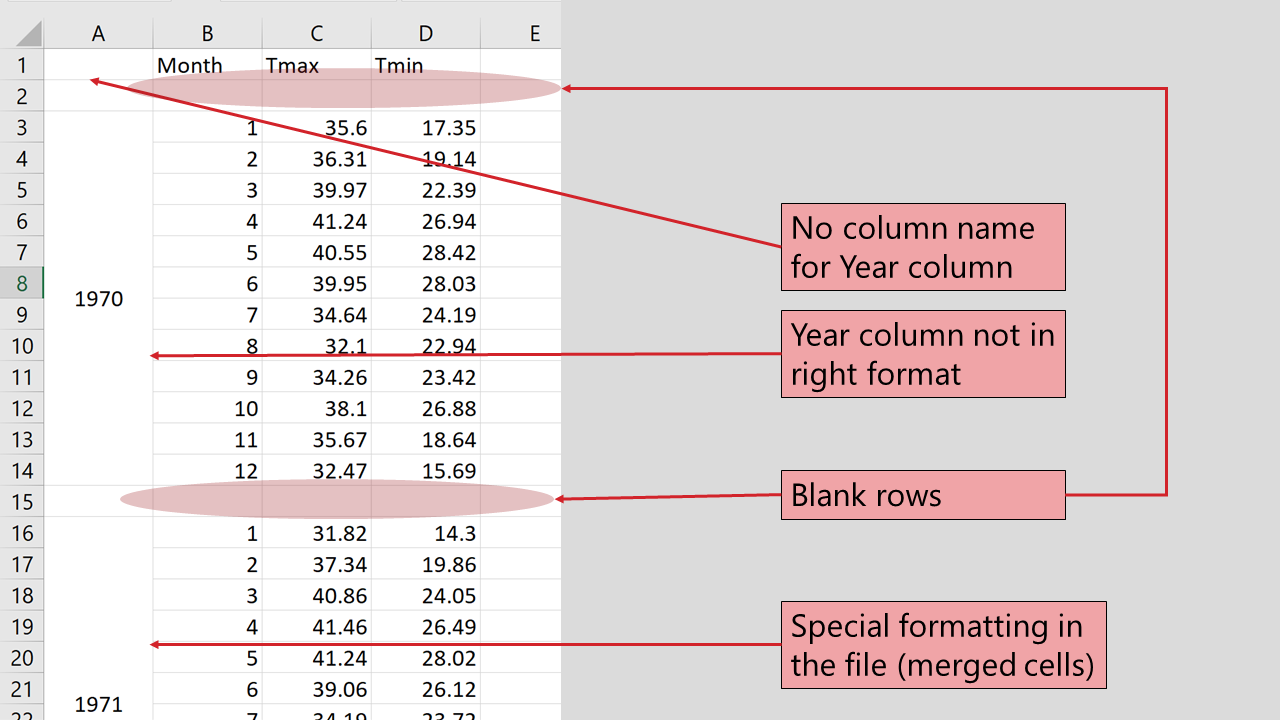
\includegraphics[width=\textwidth,height=\textheight]{Images/import1}

and here is the correted version

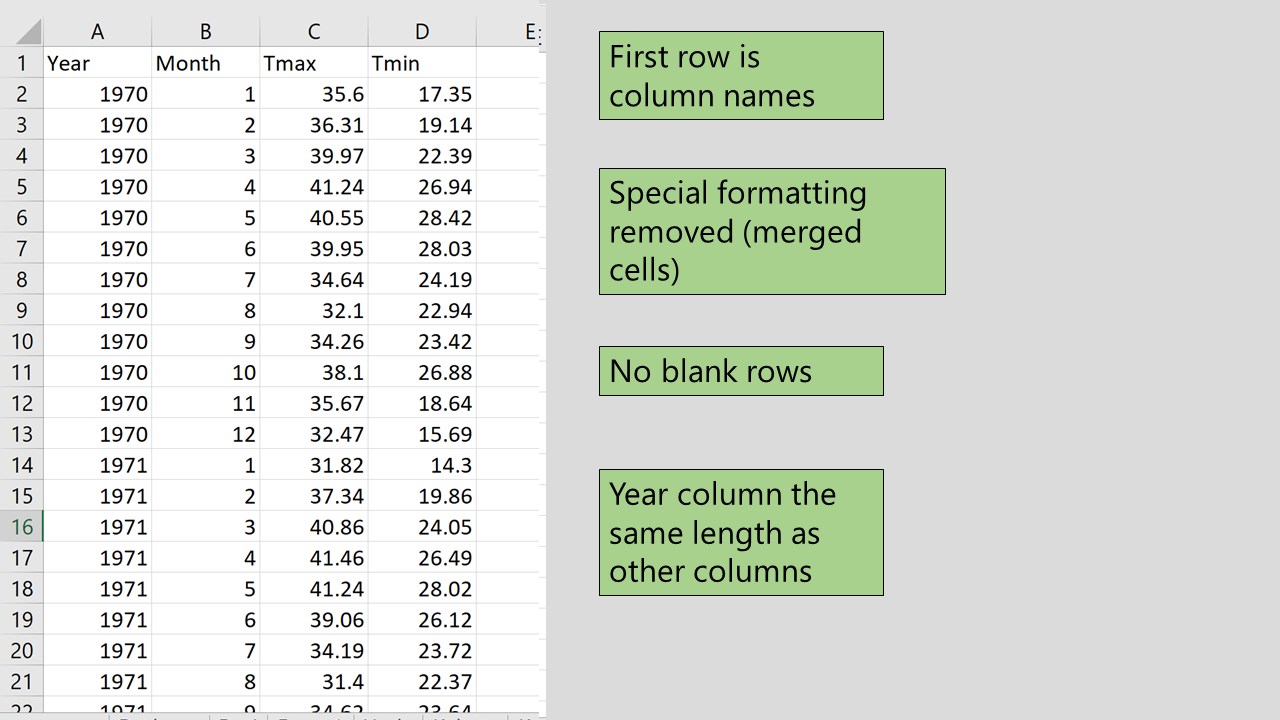
\includegraphics[width=\textwidth,height=\textheight]{Images/import2}

\hypertarget{introduction-to-ukireland-dataset}{%
\section{Introduction to UKIreland dataset}\label{introduction-to-ukireland-dataset}}

The UKIreland data contains data from 2000 to 2016 with the gdp, population, and unemployment rate of the UK and Ireland. \citep{Livestock}

\hypertarget{reading-in-data-from-csv}{%
\section{Reading in data from CSV}\label{reading-in-data-from-csv}}

CSV format is the most common formats to save data. See notes in the slides about good practice for data structures before reading anything in.

If there are problems in your data before you read it into R, there will be problems with your analysis in R. Make sure you check your data when it comes in - solving the problems in your raw data files is usually easier than solving the problems using R, and will also prevent others using the data from running into the same problems in the future.

\begin{Shaded}
\begin{Highlighting}[]
\NormalTok{UKIreland<-}\KeywordTok{read.csv}\NormalTok{(}\StringTok{"path/to/file"}\NormalTok{)}
\end{Highlighting}
\end{Shaded}

\hypertarget{reading-in-from-excel}{%
\section{Reading in from Excel}\label{reading-in-from-excel}}

Reading from excel is also easy; but needs an extra package to be installed. There are a lot of different options to do this!
My preferred choice is to use the openxlsx library.

\begin{Shaded}
\begin{Highlighting}[]
\KeywordTok{library}\NormalTok{(openxlsx)}

\NormalTok{UKIreland2<-}\KeywordTok{read.xlsx}\NormalTok{(}\StringTok{"path/to/UKIreland.xlsx"}\NormalTok{)}

\NormalTok{UKIreland2}
\end{Highlighting}
\end{Shaded}

Note that the excel version of the file is different; there is one sheet for each country.

The read.xlsx function automatically only reads in the first sheet. So this line above has only read in the data for Ireland, from the first tab in the Excel file. However, if we have named sheets in our Excel file then reading in the sheets we want is easy:

\begin{Shaded}
\begin{Highlighting}[]
\NormalTok{UK<-}\KeywordTok{read.xlsx}\NormalTok{(}\StringTok{"path/to/UKIreland.xlsx"}\NormalTok{,}\StringTok{"UK"}\NormalTok{)}
\NormalTok{Ireland<-}\KeywordTok{read.xlsx}\NormalTok{(}\StringTok{"path/to/UKIreland.xlsx"}\NormalTok{,}\StringTok{"Ireland"}\NormalTok{)}
\end{Highlighting}
\end{Shaded}

We can use \texttt{filter()} to produce subsets of our data - e.g.~to find the maximum unemployment rate:

\begin{Shaded}
\begin{Highlighting}[]
\KeywordTok{filter}\NormalTok{(UKIreland,unemployment}\OperatorTok{==}\KeywordTok{max}\NormalTok{(unemployment))}
\end{Highlighting}
\end{Shaded}

\begin{verbatim}
##   country date      gdp population unemployment capital
## 1 Ireland 2012 49177.44    4586897       14.725  Dublin
\end{verbatim}

Remember the double == when making logical statements

Using pipes and group\_by() lets us combine multiple tasks together easily - e.g.~finding the maximum unemployment rate within each country

\begin{Shaded}
\begin{Highlighting}[]
\NormalTok{UKIreland }\OperatorTok
\StringTok{  }\KeywordTok{group_by}\NormalTok{(country) }\OperatorTok
\StringTok{    }\KeywordTok{filter}\NormalTok{(unemployment}\OperatorTok{==}\KeywordTok{max}\NormalTok{(unemployment))}
\end{Highlighting}
\end{Shaded}

\begin{verbatim}
## # A tibble: 2 x 6
## # Groups:   country [2]
##   country         date    gdp population unemployment capital
##   <fct>          <int>  <dbl>      <int>        <dbl> <fct>  
## 1 Ireland         2012 49177.    4586897        14.7  Dublin 
## 2 United Kingdom  2011 41412.   63258918         8.09 London
\end{verbatim}

Or we could use summarise() to calculate average unemployment rates per country:

\begin{Shaded}
\begin{Highlighting}[]
\NormalTok{UKIreland }\OperatorTok
\StringTok{  }\KeywordTok{group_by}\NormalTok{(country) }\OperatorTok
\StringTok{    }\KeywordTok{summarise}\NormalTok{(}\DataTypeTok{average_unemployment=}\KeywordTok{mean}\NormalTok{(unemployment))}
\end{Highlighting}
\end{Shaded}

\begin{verbatim}
## # A tibble: 2 x 2
##   country        average_unemployment
##   <fct>                         <dbl>
## 1 Ireland                        8.18
## 2 United Kingdom                 6.02
\end{verbatim}

Note this time - only a single = sign in summarise because we are assigning a value (set average\_unemployment to be equal to mean of unemployment). Earlier we wanted R to check if two things were equal (when is unemployment equal to maximum unemployment), so we used \texttt{==}.

mutate() is a nice function to help us create new variables. E.g. the total number of unemployed people

\begin{Shaded}
\begin{Highlighting}[]
\KeywordTok{mutate}\NormalTok{(UKIreland,}\DataTypeTok{TotalUnemployed=}\NormalTok{unemployment}\OperatorTok{*}\NormalTok{population}\OperatorTok{/}\DecValTok{100}\NormalTok{)}
\end{Highlighting}
\end{Shaded}

\begin{tabular}{lrrrrlr}
\toprule
country & date & gdp & population & unemployment & capital & TotalUnemployed\\
\midrule
Ireland & 2000 & 26241.51 & 3805174 & 4.266667 & Dublin & 162354.1\\
Ireland & 2001 & 28227.28 & 3866243 & 3.925000 & Dublin & 151750.0\\
Ireland & 2002 & 32539.95 & 3931947 & 4.491667 & Dublin & 176610.0\\
Ireland & 2003 & 41107.03 & 3996521 & 4.616667 & Dublin & 184506.1\\
Ireland & 2004 & 47630.93 & 4070262 & 4.491667 & Dublin & 182822.6\\
\addlinespace
Ireland & 2005 & 50878.64 & 4159914 & 4.400000 & Dublin & 183036.2\\
Ireland & 2006 & 54306.91 & 4273591 & 4.525000 & Dublin & 193380.0\\
Ireland & 2007 & 61359.64 & 4398942 & 4.691667 & Dublin & 206383.7\\
Ireland & 2008 & 61257.90 & 4489544 & 6.433333 & Dublin & 288827.3\\
Ireland & 2009 & 52104.04 & 4535375 & 12.050000 & Dublin & 546512.7\\
\bottomrule
\end{tabular}

Note that this is obviously a stupid number from a methodological point of view since unemployment rates are based on ``eligible workforce population'' rather than total population. But I'm not an economist so let's go with that for now.

\hypertarget{merging-datasets}{%
\chapter{Merging datasets}\label{merging-datasets}}

\hypertarget{set-up-for-session-1}{%
\section{Set Up for Session}\label{set-up-for-session-1}}

In this session, we are going to use the following packages; \texttt{dplyr,\ ggplot2,\ openxlsx,\ tidyr,\ plotly}. If you get an error saying \texttt{there\ is\ no\ package\ called\ \_\_\_\_\_}, install the package as covered in the first tutorial.

\begin{Shaded}
\begin{Highlighting}[]
\KeywordTok{library}\NormalTok{(dplyr)}
\KeywordTok{library}\NormalTok{(ggplot2)}
\KeywordTok{library}\NormalTok{(openxlsx)}
\KeywordTok{library}\NormalTok{(tidyr)}
\KeywordTok{library}\NormalTok{(plotly)}
\end{Highlighting}
\end{Shaded}

We have used the following datasets in this tutorial. Import them as covered in the previous tutorial \texttt{UKIreland.csv,\ UKIreland.xlsx,\ UN\_LivestockData.csv,\ WorldBankData.csv}

\hypertarget{binding}{%
\section{Binding}\label{binding}}

After sucessfully loading the datasets, there should be seperate data frames of the UK data and Ireland data that we used in the previous tutorial. Ideally we would like to combine these together into a single data frame.

In this case the two data frames have the same structure; the columns are the same, the column names are the same and there are the same number of rows (one for each year).

We can use the \texttt{rbind()} function to merge the data frames together. \texttt{rbind()} attatches the rows of the second data frame below the first data frame.

\begin{Shaded}
\begin{Highlighting}[]
\NormalTok{UKIreland<-}\KeywordTok{rbind}\NormalTok{(UK,Ireland)}
\end{Highlighting}
\end{Shaded}

\texttt{rbind()} only works because the UK data has the same columns as the Ireland data. For example, we will get an error if we had calculated a new column in one dataset but not in the other:

\begin{Shaded}
\begin{Highlighting}[]
\NormalTok{UK2 <-}\StringTok{ }\KeywordTok{mutate}\NormalTok{(UK,}\DataTypeTok{pop_mill=}\NormalTok{population}\OperatorTok{/}\DecValTok{1000000}\NormalTok{)}

\KeywordTok{rbind}\NormalTok{(UK2,Ireland)}
\end{Highlighting}
\end{Shaded}

\begin{verbatim}
## Error in rbind(deparse.level, ...): numbers of columns of arguments do not match
\end{verbatim}

There is also a function called \texttt{cbind}. This binds the columns together.

\begin{Shaded}
\begin{Highlighting}[]
\NormalTok{UKIreland2<-}\KeywordTok{cbind}\NormalTok{(UK,Ireland)}
\end{Highlighting}
\end{Shaded}

\texttt{cbind()} will only work if we have the same number of rows in each data. cbind also produces a slightly confusing dataset - we now have two sets columns called ``population'', ``country'' and so on; this makes it very difficult to work with!

\texttt{rbind()} is used often but \texttt{cbind()} is not since to be useful the two datasets need to have the same number of rows with each row describing the same thing. There are more functions to allow more flexible types of merging of datasets.

\hypertarget{introducing-merging}{%
\section{Introducing merging}\label{introducing-merging}}

\texttt{dplyr} has a number of clever functions for merging data.

\begin{longtable}[]{@{}ll@{}}
\toprule
\begin{minipage}[b]{0.10\columnwidth}\raggedright
\textbf{Join function}\strut
\end{minipage} & \begin{minipage}[b]{0.84\columnwidth}\raggedright
\textbf{Description}\strut
\end{minipage}\tabularnewline
\midrule
\endhead
\begin{minipage}[t]{0.10\columnwidth}\raggedright
\texttt{full\_join()}\strut
\end{minipage} & \begin{minipage}[t]{0.84\columnwidth}\raggedright
merges two datasets and keeping all observations from both datasets\strut
\end{minipage}\tabularnewline
\begin{minipage}[t]{0.10\columnwidth}\raggedright
\texttt{inner\_join()}\strut
\end{minipage} & \begin{minipage}[t]{0.84\columnwidth}\raggedright
merges two datasets and only keeping the matching observations\strut
\end{minipage}\tabularnewline
\begin{minipage}[t]{0.10\columnwidth}\raggedright
\texttt{left\_join()}\strut
\end{minipage} & \begin{minipage}[t]{0.84\columnwidth}\raggedright
merges two datasets and keeping all observations from the first (``left'') data set but only the observations that match from the second (``right'') data set\strut
\end{minipage}\tabularnewline
\begin{minipage}[t]{0.10\columnwidth}\raggedright
\texttt{right\_join()}\strut
\end{minipage} & \begin{minipage}[t]{0.84\columnwidth}\raggedright
merges two datasets and keeping all observations from the second (``right'') data set but only the observations that match from the first (``left'') data set\strut
\end{minipage}\tabularnewline
\begin{minipage}[t]{0.10\columnwidth}\raggedright
\texttt{anti\_join()}\strut
\end{minipage} & \begin{minipage}[t]{0.84\columnwidth}\raggedright
identifying rows present in the first (``left'') dataset which do not have a match in the second (``right'') dataset.\strut
\end{minipage}\tabularnewline
\bottomrule
\end{longtable}

We will work through these sequentially. The function for merging all the data is full\_join. The key identifier column between UK and Ireland would be the ``date'' column.

\begin{Shaded}
\begin{Highlighting}[]
\KeywordTok{full_join}\NormalTok{(UK,Ireland,}\DataTypeTok{by=}\StringTok{"date"}\NormalTok{)}
\end{Highlighting}
\end{Shaded}

\begin{verbatim}
##         country.x date    gdp.x population.x unemployment.x capital.x
## 1  United Kingdom 2000 27982.36     58892514       5.450000    London
## 2  United Kingdom 2001 27427.59     59119673       5.083333    London
## 3  United Kingdom 2002 29785.99     59370479       5.175000    London
## 4  United Kingdom 2003 34173.98     59647577       5.008333    London
## 5  United Kingdom 2004 39983.98     59987905       4.750000    London
## 6  United Kingdom 2005 41732.64     60401206       4.841667    London
## 7  United Kingdom 2006 44252.32     60846820       5.416667    London
## 8  United Kingdom 2007 50134.32     61322463       5.333333    London
## 9  United Kingdom 2008 46767.59     61806995       5.708333    London
## 10 United Kingdom 2009 38262.18     62276270       7.608333    London
## 11 United Kingdom 2010 38893.02     62766365       7.891667    London
## 12 United Kingdom 2011 41412.35     63258918       8.091667    London
## 13 United Kingdom 2012 41790.78     63700300       7.991667    London
## 14 United Kingdom 2013 42724.07     64128226       7.591667    London
## 15 United Kingdom 2014 46783.47     64613160       6.200000    London
## 16 United Kingdom 2015 44305.55     65128861       5.375000    London
## 17 United Kingdom 2016 40341.41     65637239       4.900000    London
##    country.y    gdp.y population.y unemployment.y capital.y
## 1    Ireland 26241.51      3805174       4.266667    Dublin
## 2    Ireland 28227.28      3866243       3.925000    Dublin
## 3    Ireland 32539.95      3931947       4.491667    Dublin
## 4    Ireland 41107.03      3996521       4.616667    Dublin
## 5    Ireland 47630.93      4070262       4.491667    Dublin
## 6    Ireland 50878.64      4159914       4.400000    Dublin
## 7    Ireland 54306.91      4273591       4.525000    Dublin
## 8    Ireland 61359.64      4398942       4.691667    Dublin
## 9    Ireland 61257.90      4489544       6.433333    Dublin
## 10   Ireland 52104.04      4535375      12.050000    Dublin
## 11   Ireland 48671.89      4560155      13.908333    Dublin
## 12   Ireland 52224.01      4576794      14.675000    Dublin
## 13   Ireland 49177.44      4586897      14.725000    Dublin
## 14   Ireland 52060.47      4598294      13.091667    Dublin
## 15   Ireland 55899.16      4617225      11.316667    Dublin
## 16   Ireland 62139.67      4676835       9.458333    Dublin
## 17   Ireland 63861.92      4773095       7.908333    Dublin
\end{verbatim}

Notice that instead of duplicated names for the columns, we now have a suffix .x and .y. It might be useful to have a more informative suffix so that we don't have to constantly remember which country is x and which country is y.

\begin{Shaded}
\begin{Highlighting}[]
\KeywordTok{full_join}\NormalTok{(UK,Ireland,}\DataTypeTok{by=}\StringTok{"date"}\NormalTok{,}\DataTypeTok{suffix=}\KeywordTok{c}\NormalTok{(}\StringTok{"_UK"}\NormalTok{,}\StringTok{"_IRE"}\NormalTok{))}
\end{Highlighting}
\end{Shaded}

\textbf{QUESTION: In the previous chunk what we would expect to see if we were to replace full\_join() with inner\_join()?}

\hypertarget{applying-merging}{%
\section{Applying merging}\label{applying-merging}}

\hypertarget{piping-into-ggplot-some-new-geoms}{%
\subsection{Piping into ggplot (+ some new geoms)}\label{piping-into-ggplot-some-new-geoms}}

We could now make a plot of GDP in Ireland against GDP in UK. We can pipe data into a graph in a similar way to piping data commands that we saw yesterday.

\begin{Shaded}
\begin{Highlighting}[]
\KeywordTok{full_join}\NormalTok{(UK,Ireland,}\DataTypeTok{by=}\StringTok{"date"}\NormalTok{,}\DataTypeTok{suffix=}\KeywordTok{c}\NormalTok{(}\StringTok{"_UK"}\NormalTok{,}\StringTok{"_IRE"}\NormalTok{)) }\OperatorTok
\StringTok{  }\KeywordTok{ggplot}\NormalTok{(}\KeywordTok{aes}\NormalTok{(}\DataTypeTok{y=}\NormalTok{gdp_UK,}\DataTypeTok{x=}\NormalTok{gdp_IRE)) }\OperatorTok{+}
\StringTok{    }\KeywordTok{geom_point}\NormalTok{()}
\end{Highlighting}
\end{Shaded}

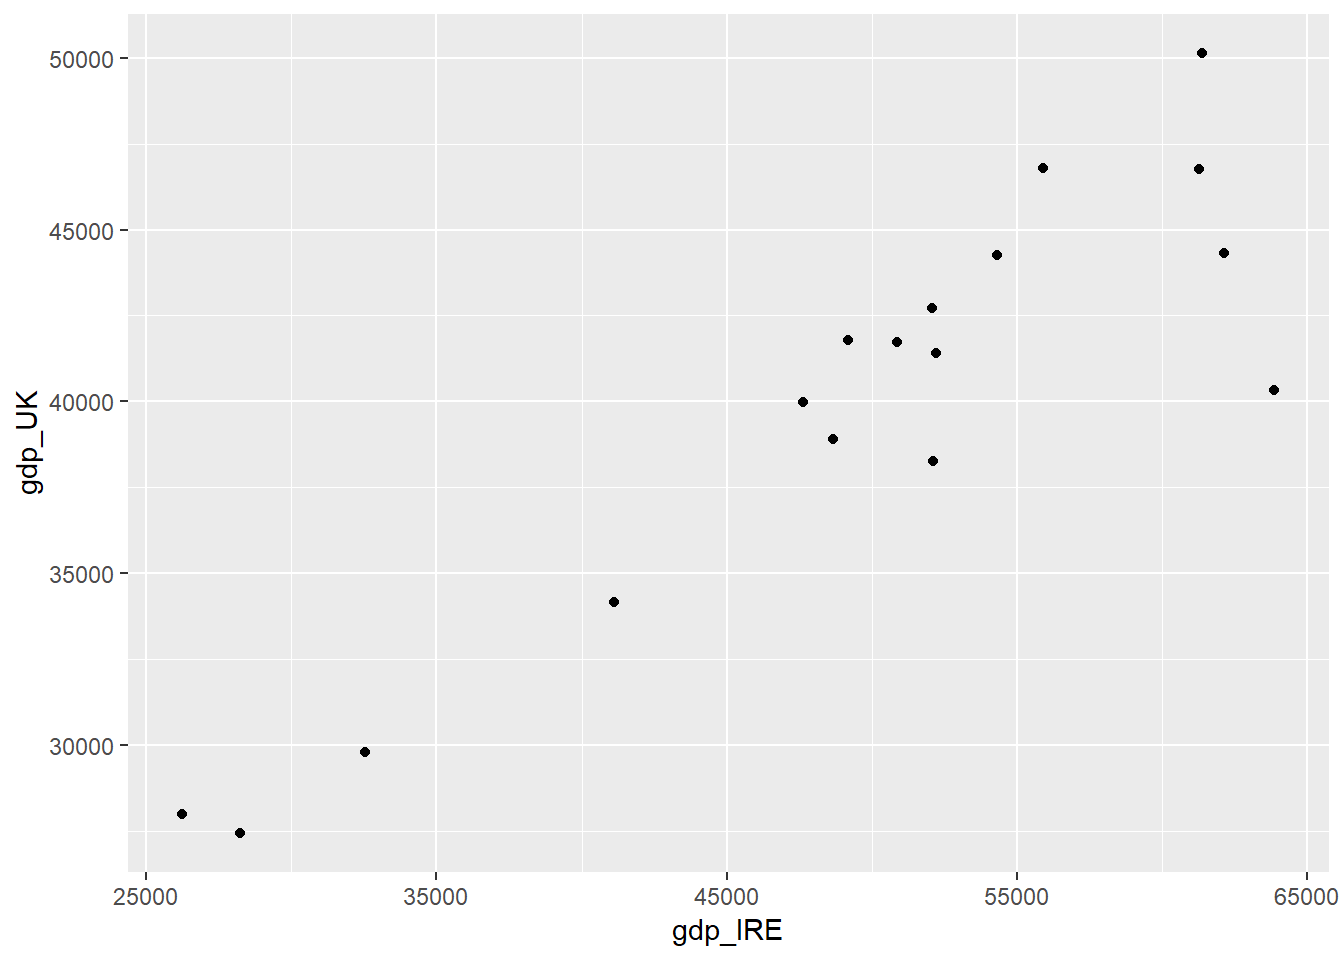
\includegraphics{Online_R_Course_files/figure-latex/unnamed-chunk-129-1.pdf}

Remember that once we have started the ggplot() we use the + to link together the components of the graph. The \%\textgreater{}\% is used to make modifications to the data.

We can also assign our plots to be named objects, similar to how we have named data frames so far. This can be a good way of sequentially building up a plot. But to actually see the plot we need to repeat back the name.

\begin{Shaded}
\begin{Highlighting}[]
\NormalTok{plot1<-}\KeywordTok{full_join}\NormalTok{(UK,Ireland,}\DataTypeTok{by=}\StringTok{"date"}\NormalTok{,}\DataTypeTok{suffix=}\KeywordTok{c}\NormalTok{(}\StringTok{"_UK"}\NormalTok{,}\StringTok{"_IRE"}\NormalTok{)) }\OperatorTok
\StringTok{  }\KeywordTok{ggplot}\NormalTok{(}\KeywordTok{aes}\NormalTok{(}\DataTypeTok{y=}\NormalTok{gdp_UK,}\DataTypeTok{x=}\NormalTok{gdp_IRE)) }\OperatorTok{+}
\StringTok{    }\KeywordTok{geom_point}\NormalTok{()}

\NormalTok{plot1}
\end{Highlighting}
\end{Shaded}

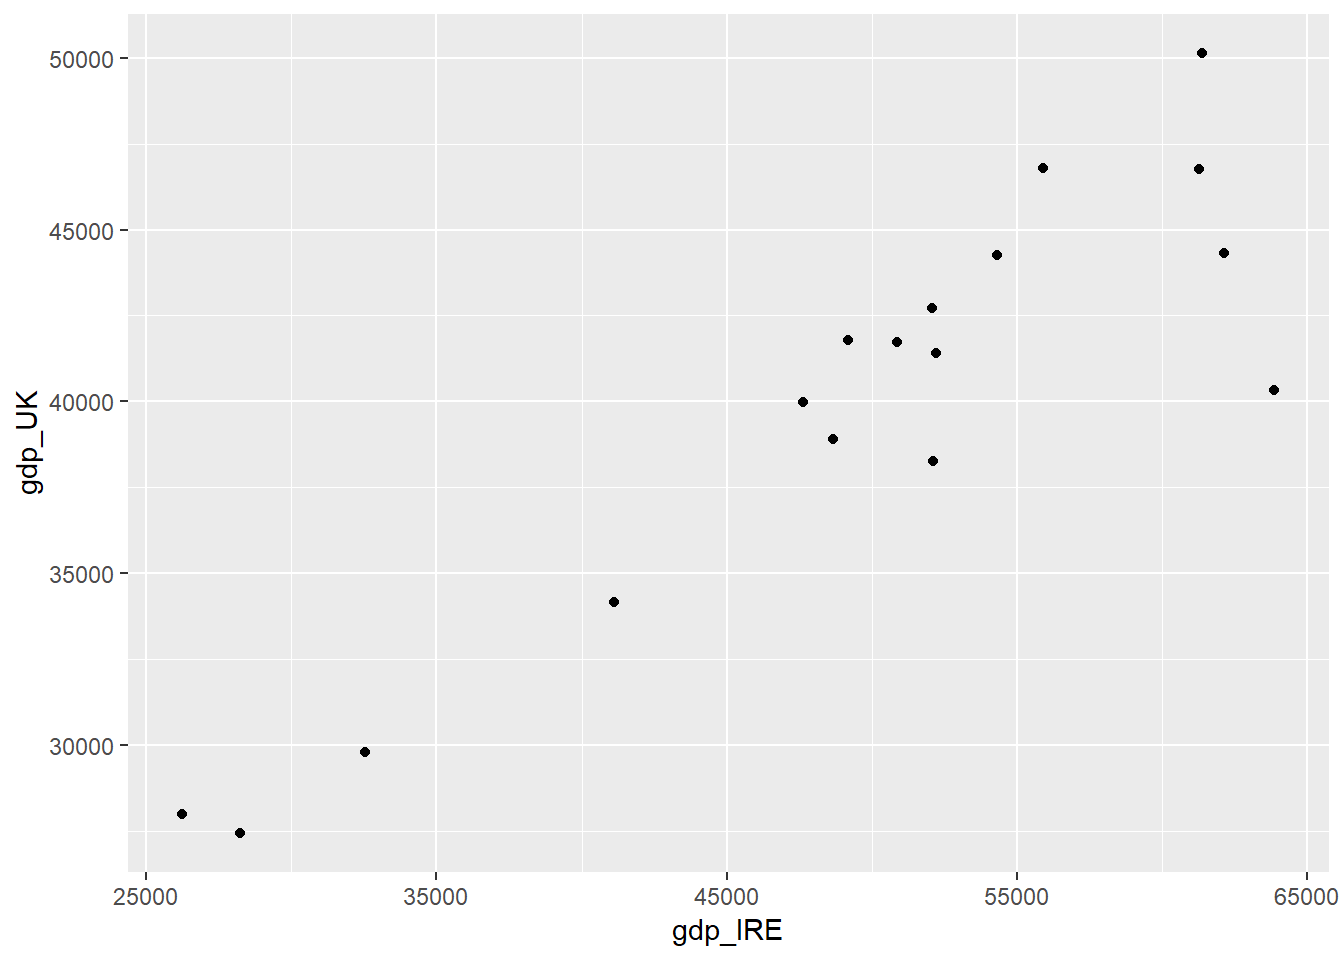
\includegraphics{Online_R_Course_files/figure-latex/unnamed-chunk-130-1.pdf}

Maybe we want to show the time dimension on this graph in some way, as each point represents a year. Yesterday we used geom\_line() to make line graphs but in this case it may not be so useful. geom\_line joins up the points from left to right. But that may not be the same order as it is from year to year. So instead we can use the function geom\_path, which joins the points in data order. If we want to be sure that the data order is sensible, we can make sure we arrange it by date first.

\begin{Shaded}
\begin{Highlighting}[]
\NormalTok{plot1}\OperatorTok{+}
\StringTok{  }\KeywordTok{geom_path}\NormalTok{()}
\end{Highlighting}
\end{Shaded}

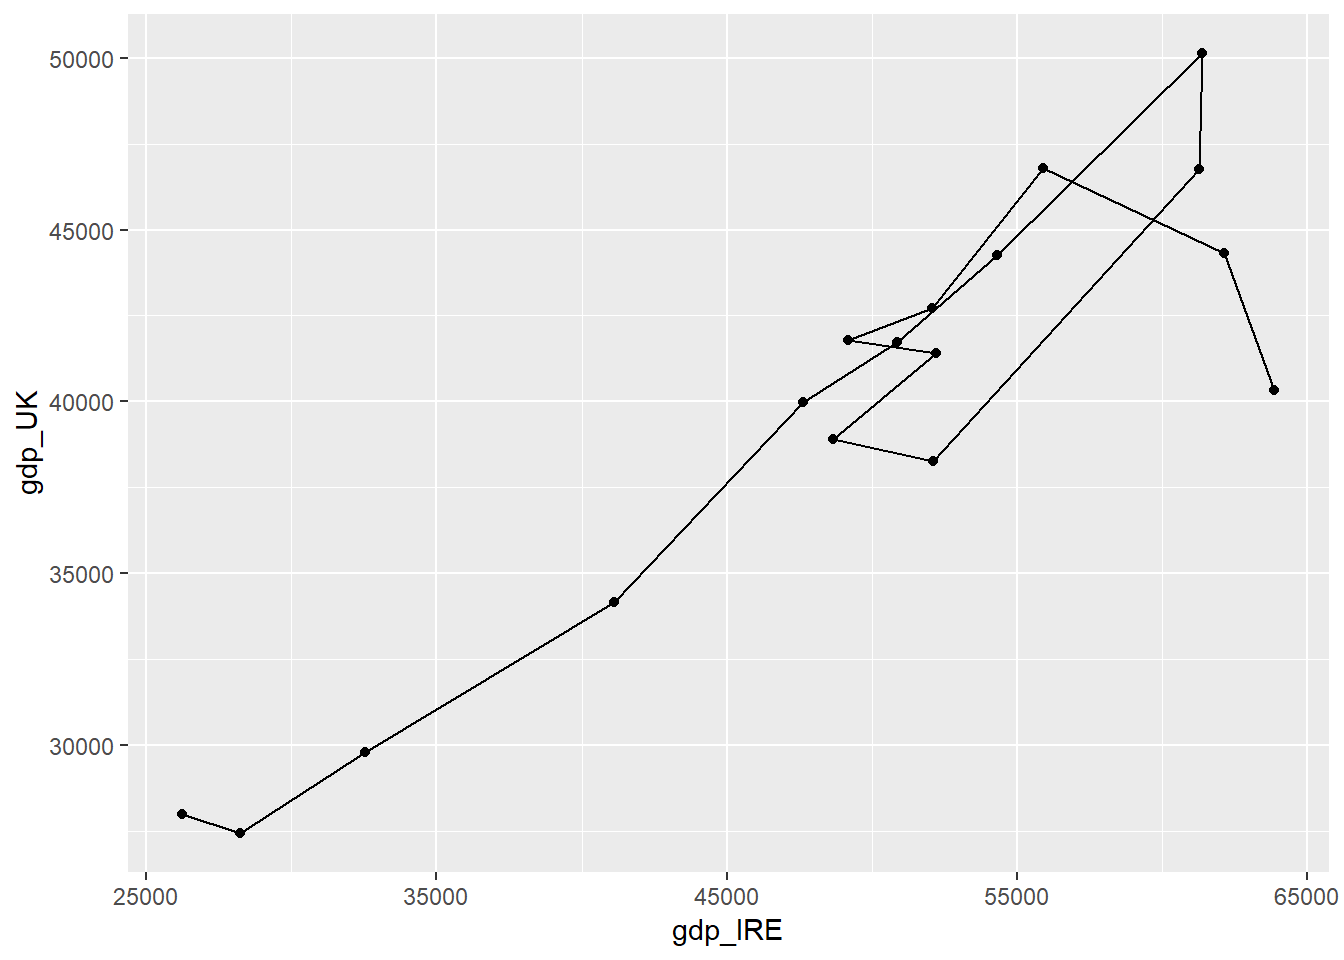
\includegraphics{Online_R_Course_files/figure-latex/unnamed-chunk-131-1.pdf}

To show this even clearer we could label the points. geom\_text() adds text to the graph. and the text column needs to be assigned to an extra aesthetic called ``label''.

\begin{Shaded}
\begin{Highlighting}[]
\NormalTok{plot1}\OperatorTok{+}
\StringTok{  }\KeywordTok{geom_path}\NormalTok{()}\OperatorTok{+}
\StringTok{    }\KeywordTok{geom_text}\NormalTok{(}\KeywordTok{aes}\NormalTok{(}\DataTypeTok{label=}\NormalTok{date))}
\end{Highlighting}
\end{Shaded}

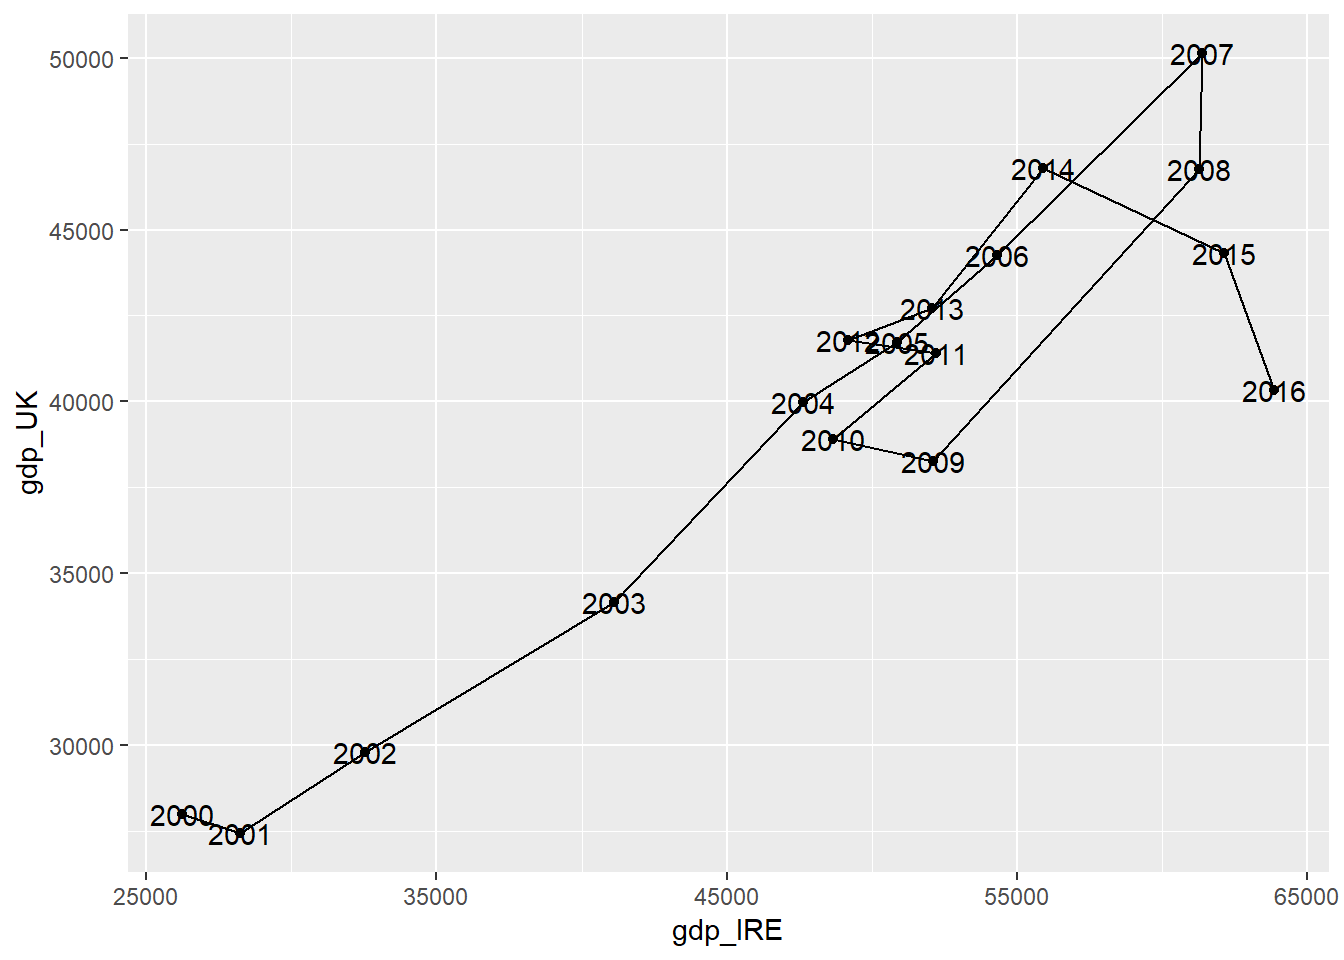
\includegraphics{Online_R_Course_files/figure-latex/unnamed-chunk-132-1.pdf}

\textbf{QUESTION: }\\
Modify the previous code to produce the same plot but;
1. colour the text labels red
2. place the labels above the points instead of on top of the points;
3. make the points bigger;
4. use a dotted line instead of a full line.
5. You might need to look into the help menus for some of these geoms to find the appropriate options, or remember the (probably even more useful) R Graphics Cookbook: \url{http://www.cookbook-r.com/Graphs/}

\begin{Shaded}
\begin{Highlighting}[]
\NormalTok{plot1}\OperatorTok{+}
\StringTok{  }\NormalTok{???}
\end{Highlighting}
\end{Shaded}

Another way of helping identify which point is which would be to use an interactive graph using the \texttt{plotly} library. This is a really easy way of making a really nice interactive graph.

To use plotly you need to assign your plot to an object, and then run ggplotly() around that object. Any information you want to be available in your interactive plot needs to be mapped to an aesthetic in the ggplot statement.

\begin{Shaded}
\begin{Highlighting}[]
\KeywordTok{ggplotly}\NormalTok{(plot1)}
\end{Highlighting}
\end{Shaded}

But these don't have to be real geoms, you can use any name and then this will be carried through to the interactive plot. E.g. - this code (suprisingly) works:

\begin{Shaded}
\begin{Highlighting}[]
\NormalTok{plot2<-}\KeywordTok{full_join}\NormalTok{(UK,Ireland,}\DataTypeTok{by=}\StringTok{"date"}\NormalTok{,}\DataTypeTok{suffix=}\KeywordTok{c}\NormalTok{(}\StringTok{"_UK"}\NormalTok{,}\StringTok{"_IRE"}\NormalTok{)) }\OperatorTok
\StringTok{  }\KeywordTok{arrange}\NormalTok{(date) }\OperatorTok
\StringTok{   }\KeywordTok{ggplot}\NormalTok{(}\KeywordTok{aes}\NormalTok{(}\DataTypeTok{y=}\NormalTok{gdp_UK,}\DataTypeTok{x=}\NormalTok{gdp_IRE,}\DataTypeTok{sgndskjgfbsljk=}\NormalTok{date)) }\OperatorTok{+}
\StringTok{    }\KeywordTok{geom_point}\NormalTok{()}\OperatorTok{+}
\StringTok{      }\KeywordTok{geom_path}\NormalTok{()}

\KeywordTok{ggplotly}\NormalTok{(plot2)}
\end{Highlighting}
\end{Shaded}

\hypertarget{challenging-merging}{%
\subsection{Challenging Merging}\label{challenging-merging}}

Let's bring in another dataset, from a different source, to do some more interesting, and difficult, merging tasks.

The Livestock data contains data from a similar period, for all countries in the world, on the number of different livestock units within that country.

Click on the dataset in the environment window to take a look at the data.

Let's try and merge this with the combined data from UK \& Ireland (UKIreland).

\textbf{QUESTION: Take a close look at these two datasets. Can you see any possible issues with trying to merge these datasets together?}

These issues can be resolved by having
i) multiple key join fields, brought together using c()
ii) changing the specification slightly - insteady of by=``key\_column\_name'' we can have \texttt{by=c("key\_column\_name\_from\_1st\_data"="key\_column\_name\_from\_2nd\_data")}.

Before running the code try to answer the following question:

\textbf{QUESTION: How many rows and columns would we expect to see in the result of each of these join statement. HINT: Check the Environment tab for lthe size of the data frames.}

\begin{Shaded}
\begin{Highlighting}[]
\KeywordTok{full_join}\NormalTok{(UKIreland,Livestock,}\DataTypeTok{by=}\KeywordTok{c}\NormalTok{(}\StringTok{"country"}\NormalTok{=}\StringTok{"Area"}\NormalTok{,}\StringTok{"date"}\NormalTok{=}\StringTok{"Year"}\NormalTok{))}

\KeywordTok{inner_join}\NormalTok{(UKIreland,Livestock,}\DataTypeTok{by=}\KeywordTok{c}\NormalTok{(}\StringTok{"country"}\NormalTok{=}\StringTok{"Area"}\NormalTok{,}\StringTok{"date"}\NormalTok{=}\StringTok{"Year"}\NormalTok{))}

\KeywordTok{anti_join}\NormalTok{(UKIreland,Livestock,}\DataTypeTok{by=}\KeywordTok{c}\NormalTok{(}\StringTok{"country"}\NormalTok{=}\StringTok{"Area"}\NormalTok{,}\StringTok{"date"}\NormalTok{=}\StringTok{"Year"}\NormalTok{))}

\KeywordTok{anti_join}\NormalTok{(Livestock,UKIreland,}\DataTypeTok{by=}\KeywordTok{c}\NormalTok{(}\StringTok{"Area"}\NormalTok{=}\StringTok{"country"}\NormalTok{,}\StringTok{"Year"}\NormalTok{=}\StringTok{"date"}\NormalTok{))}
\end{Highlighting}
\end{Shaded}

\textbf{QUESTION: We are interested in comparing the livestock populations of Ireland and the UK. Which of these options would be the most useful of these joins to use for further analysis? Assign the most useful join to an object called UKIrelandLivestock}

\begin{Shaded}
\begin{Highlighting}[]
\NormalTok{UKIrelandLivestock<-}
\end{Highlighting}
\end{Shaded}

\hypertarget{reshaping-data}{%
\chapter{Reshaping Data}\label{reshaping-data}}

Let's say you and a colleauge are asked to support data analysis of a school. You are asked to look at the grades of five students. For each student you need to look at the their grades in different subjects.

You both go away, collect your data and come back to share your results. The image below are the tables of your result. They may look different but these two datasets are showing the same information. They different only in shape; one is wide and the other is long.

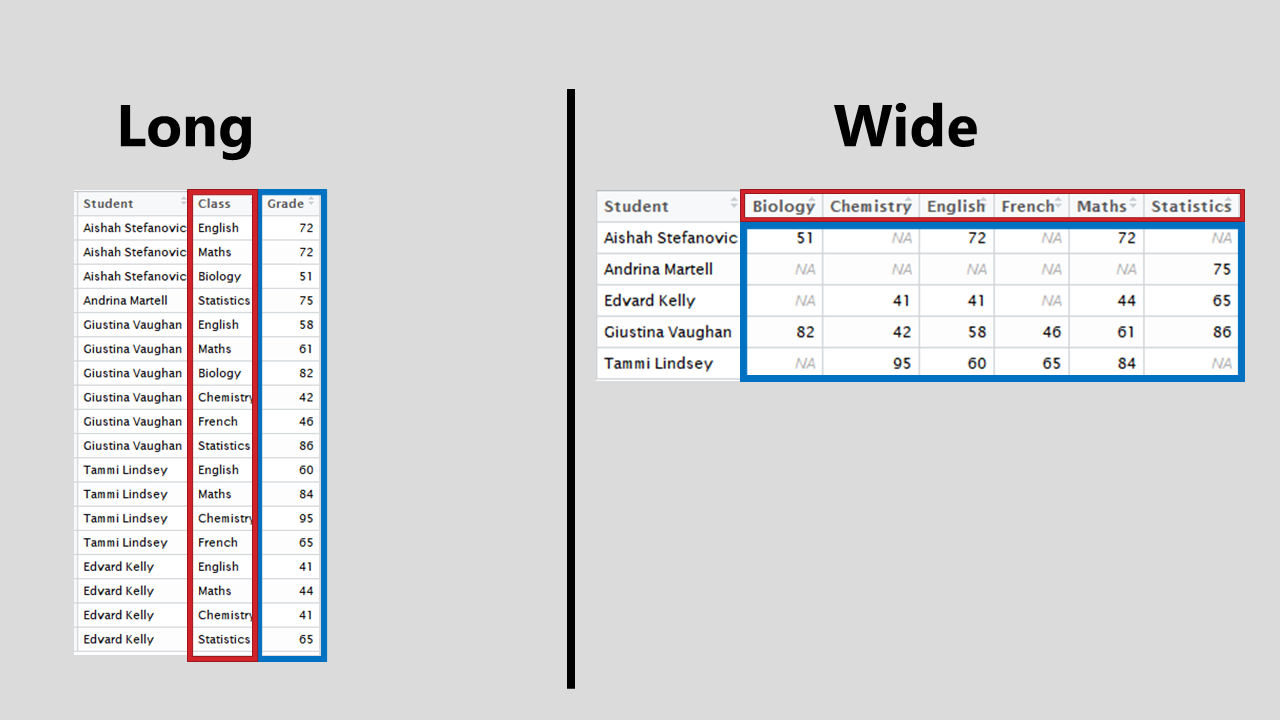
\includegraphics[width=17.78in]{Images/longandwide}

Long data sets are preferrable when working on the data on a computer whereas wide formatted data works best when presenting this information. It is unlikely the problem you will be working will provide you with perfectly formatted datasets, so it is helpful to know how to move between these shapes.

\texttt{tidyr} is a R package that aims to solve this problem by adding two useful ``words'' to our vocabulary \texttt{gather()} and \texttt{spread()}.

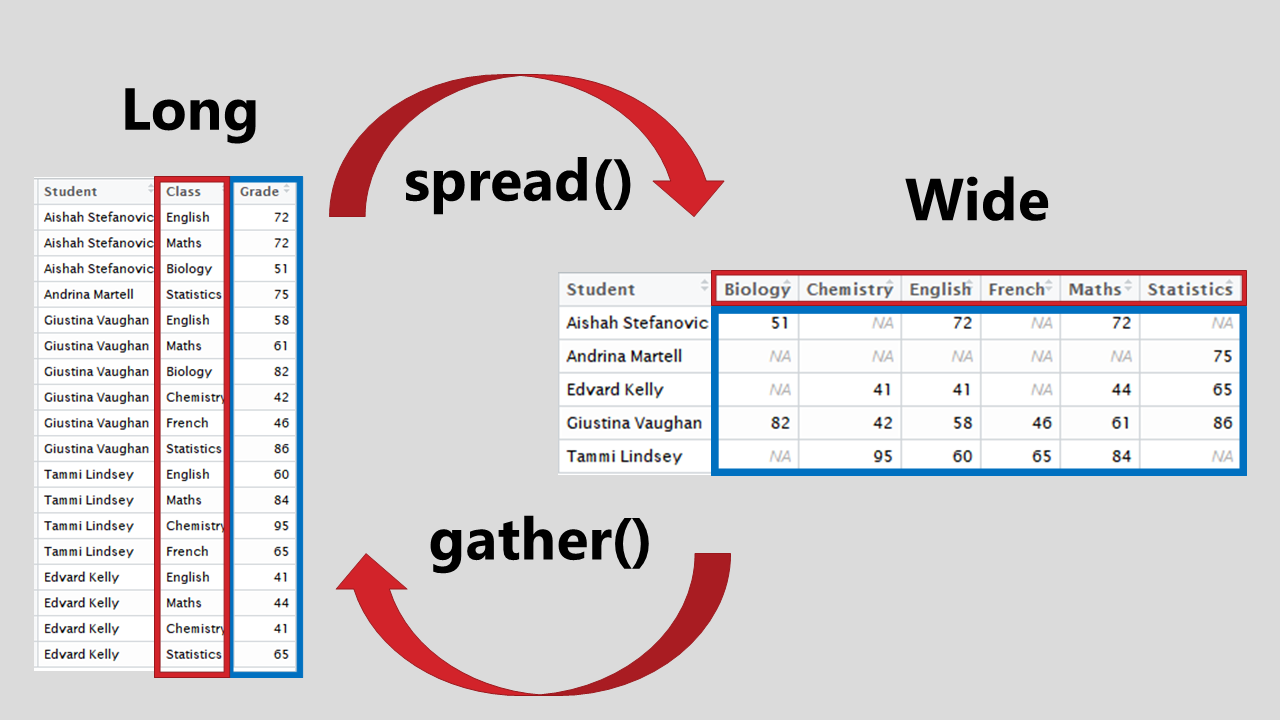
\includegraphics[width=17.78in]{Images/converting}

For these functions, you need to identify two things; \textbf{key} and \textbf{value}. \textbf{key} is the identifier and \textbf{value} are the measurements. In the example, the \textbf{key} identifier is \texttt{Class}, highlighted in red and \textbf{value} are the \texttt{Grades}, highlighted in blue.

\hypertarget{going-long}{%
\section{Going Long}\label{going-long}}

Let's try to apply these concepts to the the dataset we merged together in the last tutorial.

After loading the UK and Ireland data sets, run the code below to merge the datasets into one.

\begin{Shaded}
\begin{Highlighting}[]
\NormalTok{UKIrelandLivestock<-}\KeywordTok{inner_join}\NormalTok{(UKIreland,Livestock,}\DataTypeTok{by=}\KeywordTok{c}\NormalTok{(}\StringTok{"country"}\NormalTok{=}\StringTok{"Area"}\NormalTok{,}\StringTok{"date"}\NormalTok{=}\StringTok{"Year"}\NormalTok{))}
\end{Highlighting}
\end{Shaded}

\begin{verbatim}
## Warning: Column `country`/`Area` joining character vector and factor,
## coercing into character vector
\end{verbatim}

Our task is to adjust the number of livestock in each category for the country population. This might provide a fairer comparison between the UK and Ireland over time.

\textbf{QUESTION: Write a line of code to calculate a column containing the number of Turkeys per capita in the merged dataset}

Currently our livestock information is in wide format: one column for each type of livestock containing the values. For our data processing it would be more efficient to work with data in long format: two columns - the first containing an identifier for livestock type and the second containing the values.

We could apply a similar function on every single livestock column in our data. This would be quite tedious! Or we could \texttt{gather()} our livestock columns together and then divide one single column by the population.

There are 3 arguments which are required for \texttt{gather()};

\begin{itemize}
\item
  The first is the new name for the column which will contain the \textbf{key}. This will take the values that are currently assigned to the column names.
\item
  The second is the new name for the column which wil contain the \textbf{values}, which will contain the data values from the columns.
\item
  The third is to identify which columns to include. If these columns are sequential we can use a shortcut by using a colon and saying: FirstColumn:LastColumn
\end{itemize}

An option to use in our function is \texttt{na.rm=TRUE}. This will remove any missing values from our data. There are no camels as livestock in the British Isles, so adding this option will remove the rows about camels from the data

\begin{Shaded}
\begin{Highlighting}[]
\NormalTok{UKIrelandLivestock }\OperatorTok
\StringTok{  }\KeywordTok{gather}\NormalTok{(}\StringTok{"livestock"}\NormalTok{,}\StringTok{"total"}\NormalTok{,Beehives}\OperatorTok{:}\NormalTok{Turkeys,}\DataTypeTok{na.rm=}\OtherTok{TRUE}\NormalTok{)}
\end{Highlighting}
\end{Shaded}

The same could also have been achived by fully specifying each of the columns to be gathered, and only choosing the animals relevant to the British Isles

\begin{Shaded}
\begin{Highlighting}[]
\NormalTok{UKIrelandLivestock }\OperatorTok
\StringTok{  }\KeywordTok{gather}\NormalTok{(}\StringTok{"livestock"}\NormalTok{,}\StringTok{"total"}\NormalTok{,Cattle,Chickens,Ducks,Goats,Horses,Pigs,Sheep,Turkeys)}
\end{Highlighting}
\end{Shaded}

\textbf{QUESTIONS: Extend the previous line to add in a column of livestock per capita using the mutate function and assign it to a new object called UKIrelandLivestockCap}

\begin{Shaded}
\begin{Highlighting}[]
\NormalTok{UKIrelandLivestockCap<-}
\StringTok{  }\NormalTok{UKIrelandLivestock }\OperatorTok
\StringTok{  }\KeywordTok{gather}\NormalTok{(}\StringTok{"livestock"}\NormalTok{,}\StringTok{"total"}\NormalTok{,Beehives}\OperatorTok{:}\NormalTok{Turkeys,}\DataTypeTok{na.rm=}\OtherTok{TRUE}\NormalTok{) }\OperatorTok
\StringTok{  }\NormalTok{?????}
\end{Highlighting}
\end{Shaded}

Gathering multiple columns is also a really useful way to be able to plot multiple variables in the same ggplot.

\begin{Shaded}
\begin{Highlighting}[]
\NormalTok{UKIrelandLivestockCap }\OperatorTok\StringTok{ }
\StringTok{    }\KeywordTok{ggplot}\NormalTok{(}\KeywordTok{aes}\NormalTok{(}\DataTypeTok{y=}\NormalTok{LivestockperCapita,}\DataTypeTok{x=}\NormalTok{date,}\DataTypeTok{colour=}\NormalTok{country))}\OperatorTok{+}
\StringTok{        }\KeywordTok{geom_line}\NormalTok{()}\OperatorTok{+}
\StringTok{          }\KeywordTok{facet_wrap}\NormalTok{(}\OperatorTok{~}\NormalTok{livestock)}
\end{Highlighting}
\end{Shaded}

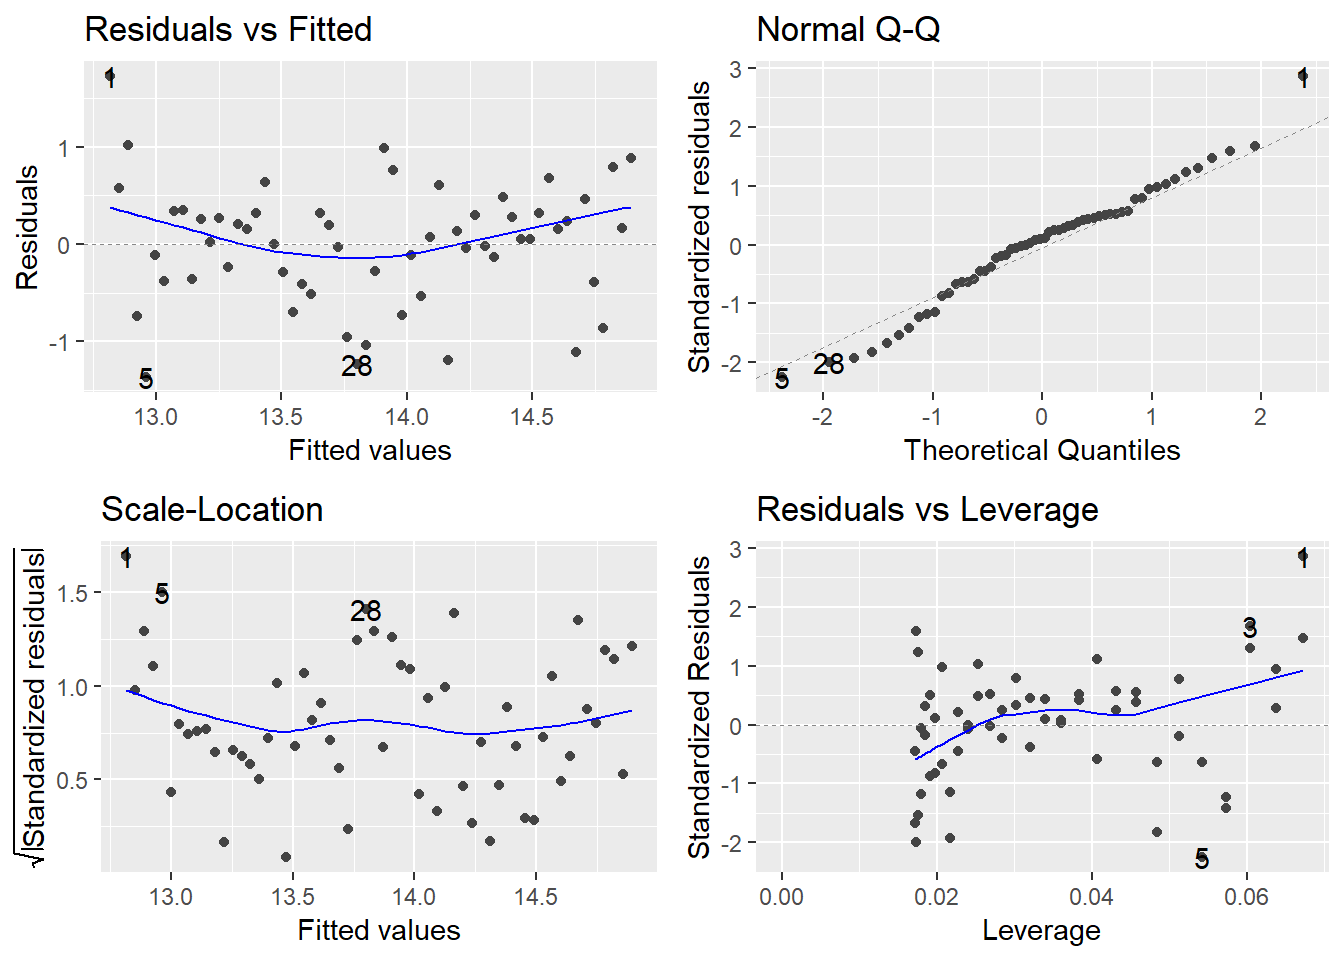
\includegraphics{Online_R_Course_files/figure-latex/unnamed-chunk-148-1.pdf}

\textbf{Did this work for you?}
\textbf{If not why not? - what needs to be changed?}

This graph is a little confusing right now. Too many of the animals have very small numbers so are effectively invisible.

So let's make it better - we can set our facets to have different scales using the option scales=``free''

\begin{Shaded}
\begin{Highlighting}[]
\NormalTok{UKIrelandLivestockCap }\OperatorTok\StringTok{ }
\StringTok{    }\KeywordTok{ggplot}\NormalTok{(}\KeywordTok{aes}\NormalTok{(}\DataTypeTok{y=}\NormalTok{LivestockperCapita,}\DataTypeTok{x=}\NormalTok{date,}\DataTypeTok{colour=}\NormalTok{country))}\OperatorTok{+}
\StringTok{        }\KeywordTok{geom_line}\NormalTok{()}\OperatorTok{+}
\StringTok{          }\KeywordTok{facet_wrap}\NormalTok{(}\OperatorTok{~}\NormalTok{livestock,}\DataTypeTok{scales=}\StringTok{"free"}\NormalTok{)}
\end{Highlighting}
\end{Shaded}

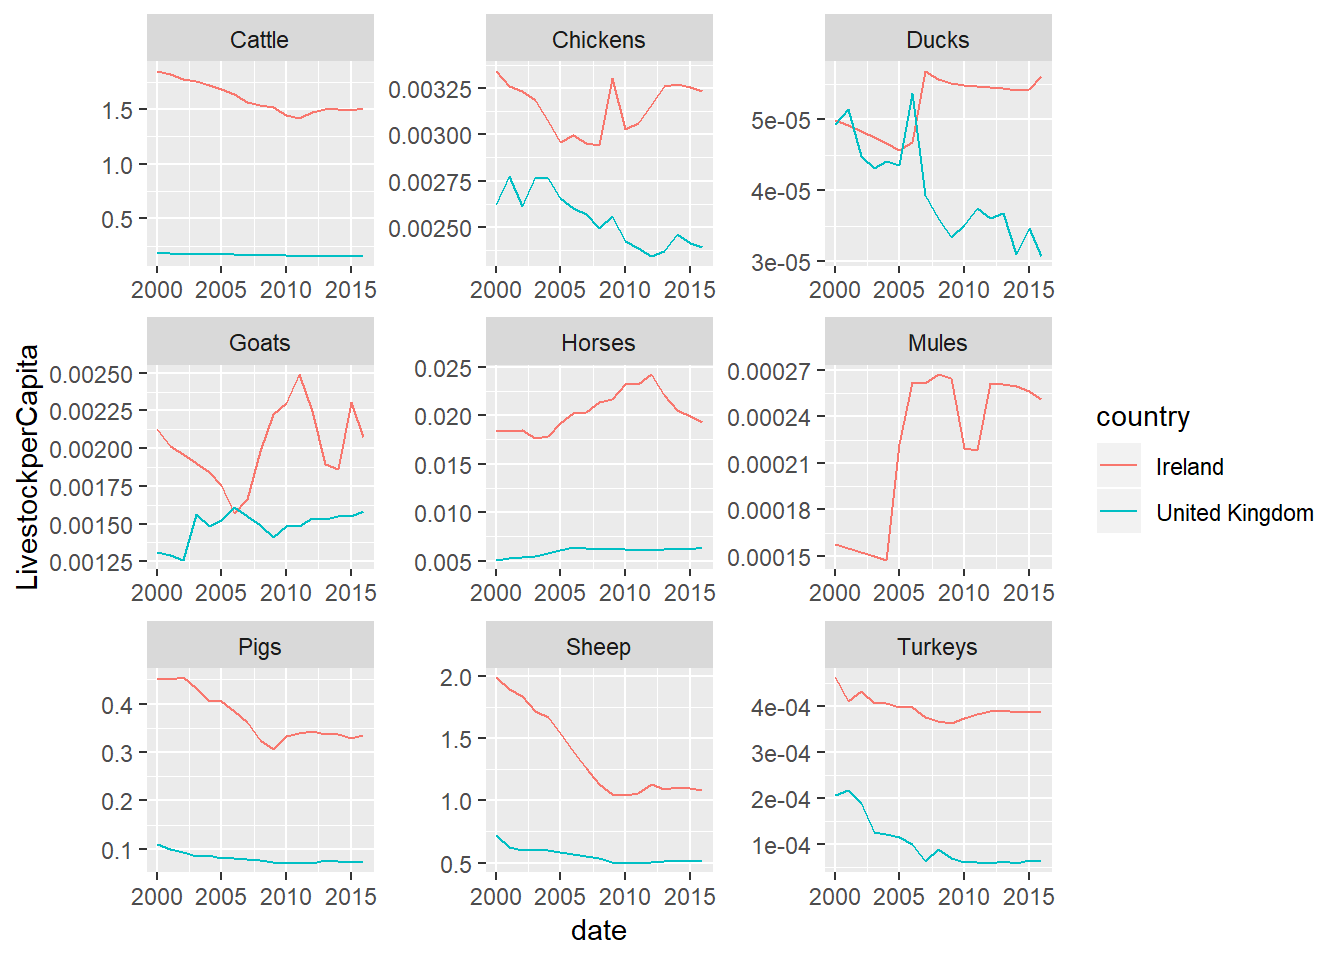
\includegraphics{Online_R_Course_files/figure-latex/unnamed-chunk-149-1.pdf}

One thing you probably noticed (other than the fact that the sheep population is declining at an alarming rate), is that this graph is a little bit squashed in at the moment within the RMD file. You can press the small square button in the top right corner of the plot to open a new window to view, and re-size the graph. It's best to use a little bit of trial and error to get a graph the size you want it to be.

\hypertarget{going-wide}{%
\section{Going wide}\label{going-wide}}

When presenting results, we usually want to put the data back into a wide format as this is easier for humans to read.

Let's say we would like to present the cattle per capita figures for UK and Ireland over the time period.

Spread requires two arguments.

The first is the column containing the identifying information. Each unique value in this column will be a column name in our wide data

The second is the column containing the corresponding values. These will form the data within each column in the wide data.

\begin{Shaded}
\begin{Highlighting}[]
\NormalTok{UKIrelandLivestockCap }\OperatorTok
\StringTok{     }\KeywordTok{filter}\NormalTok{(livestock}\OperatorTok{==}\StringTok{"Cattle"}\NormalTok{) }\OperatorTok
\StringTok{       }\KeywordTok{select}\NormalTok{(date,country,LivestockperCapita) }\OperatorTok
\StringTok{         }\KeywordTok{spread}\NormalTok{(country,LivestockperCapita)}
\end{Highlighting}
\end{Shaded}

\textbf{QUESTION: What happens if you do not include the select() line in the code? Can you explain why?}

\begin{Shaded}
\begin{Highlighting}[]
\NormalTok{UKIrelandLivestockCap }\OperatorTok
\StringTok{     }\KeywordTok{filter}\NormalTok{(livestock}\OperatorTok{==}\StringTok{"Cattle"}\NormalTok{) }\OperatorTok
\StringTok{         }\KeywordTok{spread}\NormalTok{(country,LivestockperCapita)}
\end{Highlighting}
\end{Shaded}

\hypertarget{exercises}{%
\subsection{Exercises}\label{exercises}}

\textbf{QUESTION Read in the data frame used in the lecture notes with the information from a school database of classes, grades and students. This can be found at: \url{http://shiny.stats4sd.org/Reading_R/Class} Data.xlsx or in the data folder in RStudio Cloud}

\begin{Shaded}
\begin{Highlighting}[]
\NormalTok{Grades<-}
\NormalTok{Classes<-}
\NormalTok{Students<-}
\end{Highlighting}
\end{Shaded}

\textbf{QUESTION: Using the example from the lecture notes summarising the average grade in each class as a starting point (reproduced below): i) Produce a summary of the average grade achieved by each student; ii) The number of classes that student attended; iii) Then merge this data with the Students data frame containing the student-level information}

\begin{Shaded}
\begin{Highlighting}[]
\NormalTok{Grades }\OperatorTok
\StringTok{  }\KeywordTok{group_by}\NormalTok{(Class) }\OperatorTok
\StringTok{    }\KeywordTok{summarise}\NormalTok{(}\DataTypeTok{GradeAverage=}\KeywordTok{mean}\NormalTok{(Grade) ,}\DataTypeTok{Students=}\KeywordTok{n}\NormalTok{()) }\OperatorTok
\StringTok{        }\KeywordTok{full_join}\NormalTok{(Classes,}\DataTypeTok{by=}\StringTok{"Class"}\NormalTok{)}
\end{Highlighting}
\end{Shaded}

\textbf{QUESTION: From the Livestock dataset produce a table with one column for each year showing the total number of Chickens for France}

\begin{Shaded}
\begin{Highlighting}[]
\NormalTok{Livestock }\OperatorTok
\StringTok{  }\KeywordTok{filter}\NormalTok{() }\OperatorTok
\StringTok{    }\KeywordTok{select}\NormalTok{() }\OperatorTok
\StringTok{      }\KeywordTok{spread}\NormalTok{()}
\end{Highlighting}
\end{Shaded}

\textbf{QUESTION: From the UKIreland data gather the columns gdp, population and unemployment to be able to produce a facetted plot showing all of these variables over time for the UK and Ireland}

\begin{Shaded}
\begin{Highlighting}[]
\NormalTok{UKIreland }\OperatorTok
\StringTok{  }\KeywordTok{gather}\NormalTok{() }\OperatorTok
\StringTok{    }\KeywordTok{ggplot}\NormalTok{(}\KeywordTok{aes}\NormalTok{()) }\OperatorTok{+}
\StringTok{      }\KeywordTok{facet_wrap}\NormalTok{()}\OperatorTok{+}
\StringTok{        }\KeywordTok{geom_XXXX}\NormalTok{()}
\end{Highlighting}
\end{Shaded}

\hypertarget{modelling}{%
\chapter{Modelling}\label{modelling}}

\hypertarget{set-up-for-session-2}{%
\section{Set Up for Session}\label{set-up-for-session-2}}

Packages used = ggplot2, ciTools, dplyr, ggfortify
Data used: eastbournedata.csv

\begin{Shaded}
\begin{Highlighting}[]
\KeywordTok{library}\NormalTok{(dplyr)}
\KeywordTok{library}\NormalTok{(ggplot2)}
\KeywordTok{library}\NormalTok{(ciTools)}
\KeywordTok{library}\NormalTok{(ggfortify)}

\NormalTok{eastbourne<-}\KeywordTok{read.csv}\NormalTok{(}\StringTok{"C:/Users/FaheemAshraf/Dropbox (SSD)/Faheem_workings/2018-11-22 - R Course Editing/Book version files/Data/eastbournedata.csv"}\NormalTok{)}
\end{Highlighting}
\end{Shaded}

\hypertarget{exploring-data}{%
\section{Exploring Data}\label{exploring-data}}

The data for this example is taken from the UK Met office and contains the average daily maximum temperatures, minimum temperatures and rainfall for all years since 1959.

\begin{Shaded}
\begin{Highlighting}[]
\NormalTok{plot1<-}\KeywordTok{ggplot}\NormalTok{(}\DataTypeTok{data=}\NormalTok{eastbourne,}\KeywordTok{aes}\NormalTok{(}\DataTypeTok{y=}\NormalTok{tmax,}\DataTypeTok{x=}\NormalTok{yyyy))}\OperatorTok{+}
\StringTok{  }\KeywordTok{geom_point}\NormalTok{()}
\NormalTok{plot1}
\end{Highlighting}
\end{Shaded}

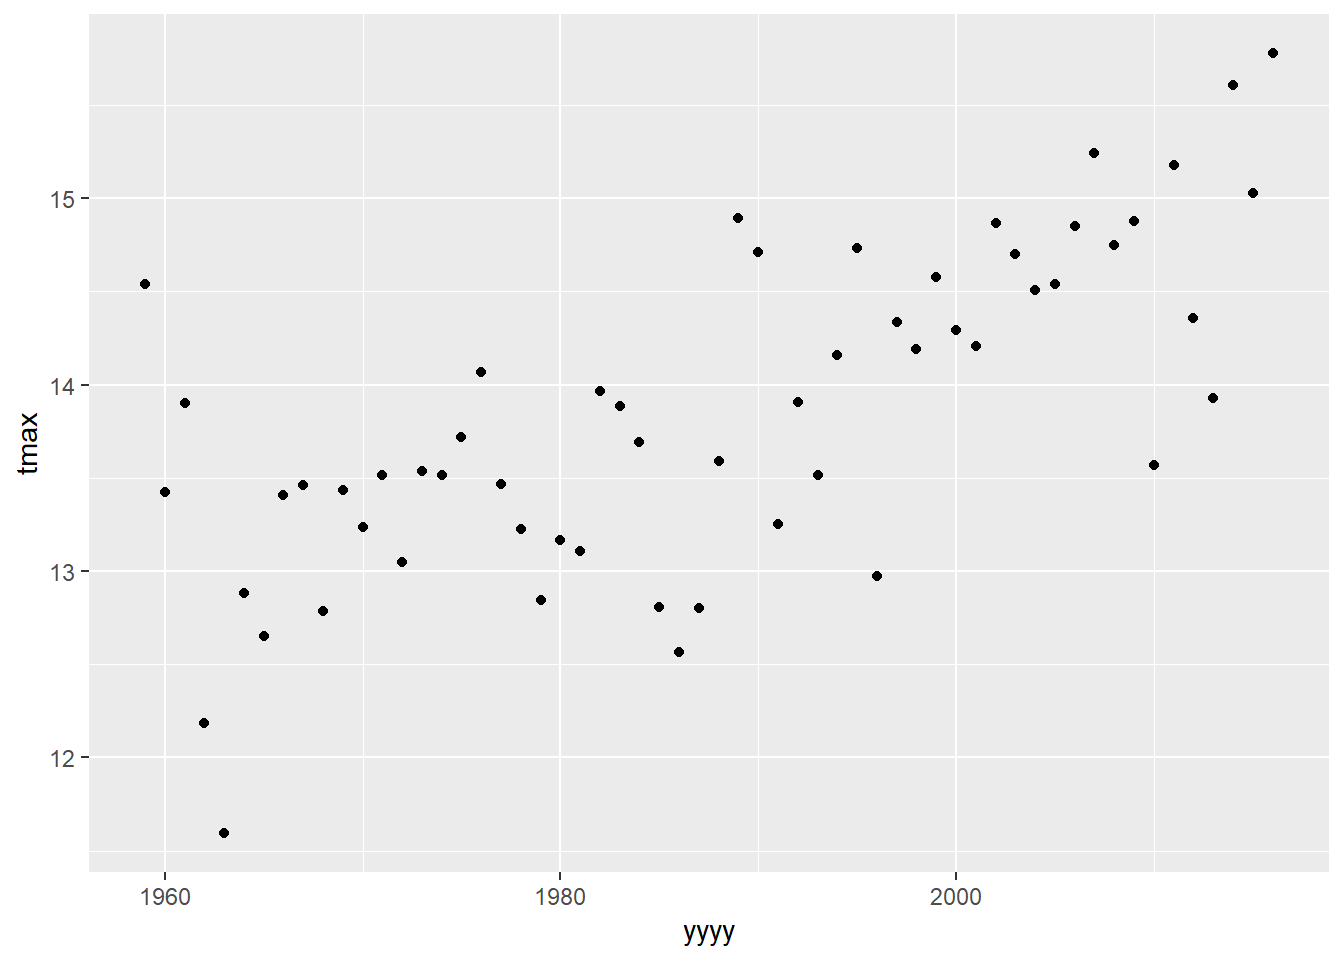
\includegraphics{Online_R_Course_files/figure-latex/unnamed-chunk-157-1.pdf}

What would be our initial thoughts about the relationship between temperature and time in Eastbourne?

\texttt{geom\_smooth} is a nice way to add on simple models to your plot that we have seen before.

\begin{Shaded}
\begin{Highlighting}[]
\NormalTok{plot1 }\OperatorTok{+}
\StringTok{    }\KeywordTok{geom_smooth}\NormalTok{()}
\end{Highlighting}
\end{Shaded}

\begin{verbatim}
## `geom_smooth()` using method = 'loess' and formula 'y ~ x'
\end{verbatim}

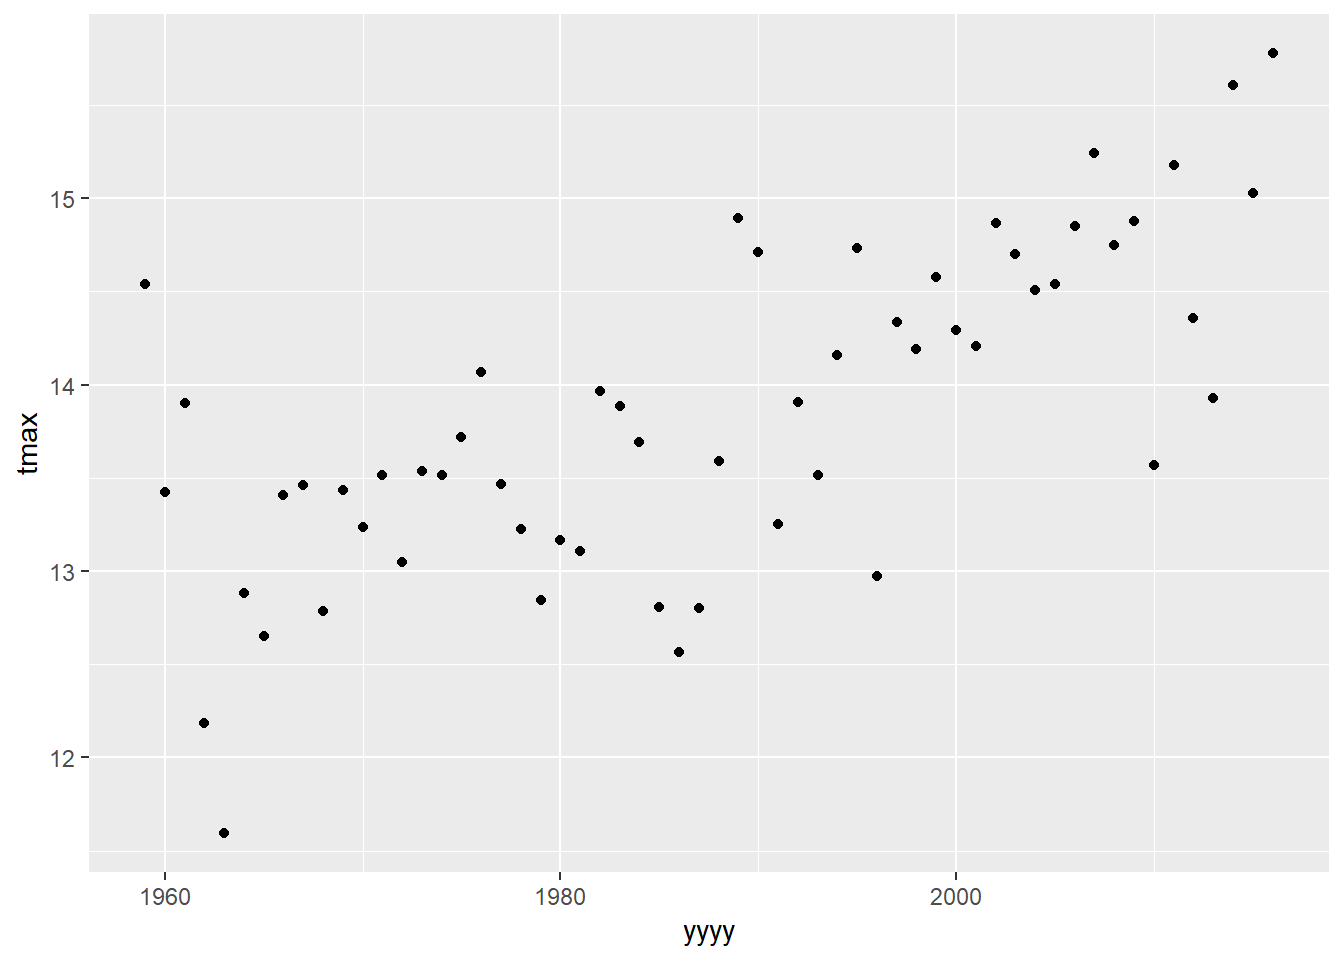
\includegraphics{Online_R_Course_files/figure-latex/unnamed-chunk-158-1.pdf}

The default model fitted by geom\_smooth depends on the amount of data being plotted. In this case it has told us that it is using a ``loess'' model to fit the line - this is a simple form of a moving average smoother. It can be useful for visualising trends that do not fit into other models, but they cannot be used for extensive statistical inference.

Lets use a more familiar model by changing the ``method'' option into a simple linear regression:

\begin{Shaded}
\begin{Highlighting}[]
\NormalTok{plot1 }\OperatorTok{+}
\StringTok{    }\KeywordTok{geom_smooth}\NormalTok{(}\DataTypeTok{method=}\StringTok{"lm"}\NormalTok{)}
\end{Highlighting}
\end{Shaded}

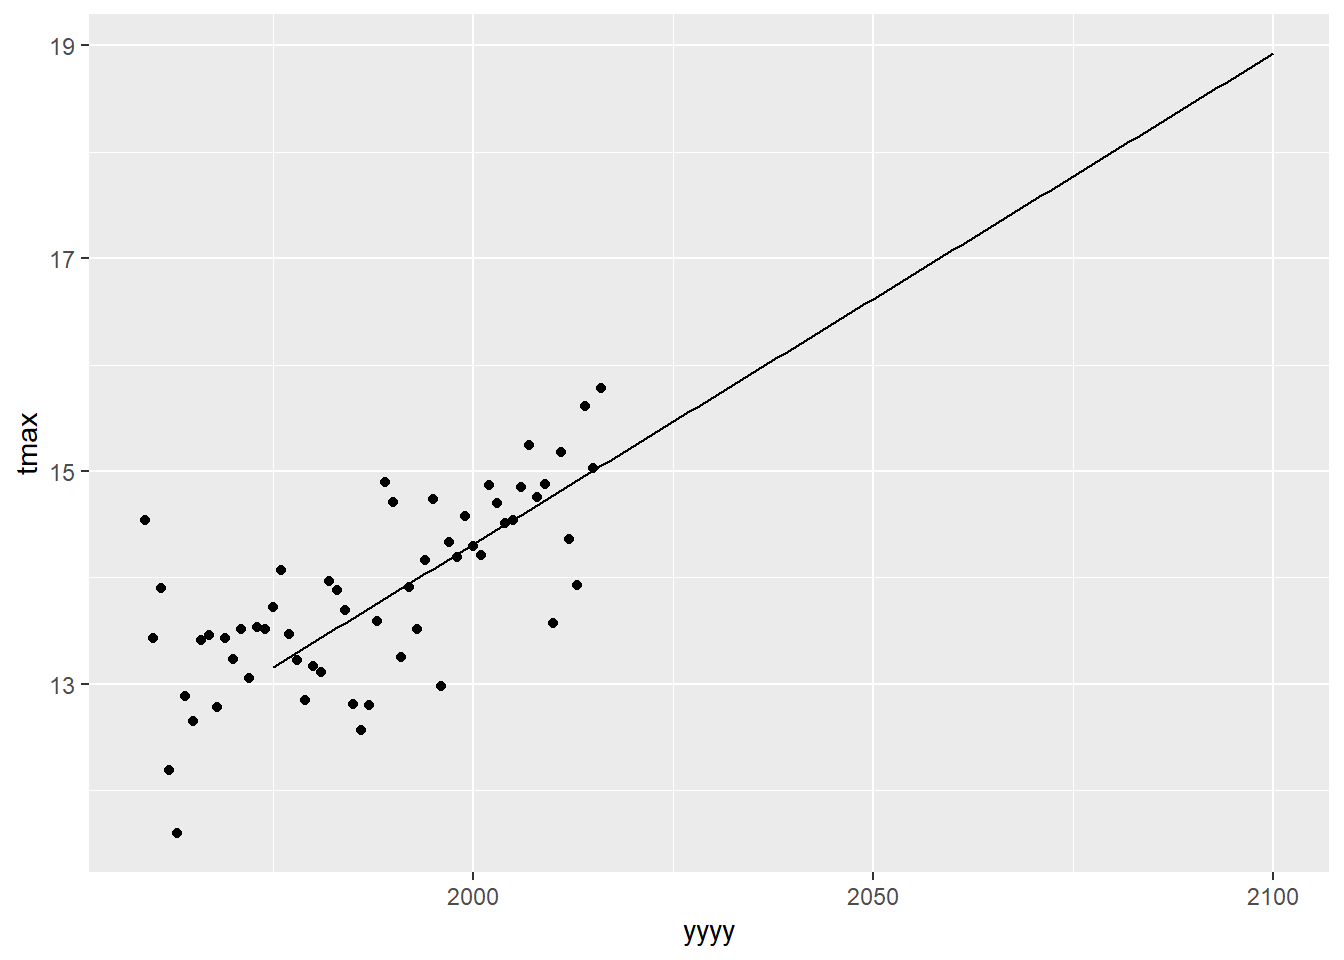
\includegraphics{Online_R_Course_files/figure-latex/unnamed-chunk-159-1.pdf}

\hypertarget{fitting-model}{%
\section{Fitting Model}\label{fitting-model}}

To examine what we actually have in our model we need to fit the model using the lm() command:

\begin{Shaded}
\begin{Highlighting}[]
\KeywordTok{lm}\NormalTok{(tmax}\OperatorTok{~}\NormalTok{yyyy,}\DataTypeTok{data=}\NormalTok{eastbourne)}
\end{Highlighting}
\end{Shaded}

\begin{verbatim}
## 
## Call:
## lm(formula = tmax ~ yyyy, data = eastbourne)
## 
## Coefficients:
## (Intercept)         yyyy  
##   -58.58684      0.03645
\end{verbatim}

The output by default only tells us two things:
``Call'' - simply repeating back the model we have specified
``Coefficients'': Telling us the values of the parameters

A linear regression follows the equation of a straight line y = B0 + B1x (or y=a+bx or y=mx+c ; depending on where and when you were 12 years old)
The coefficients give us the value of our intercept: -58.6 and the value of our slope: 0.036. So the overall model would be:

tmax = -58.6 + 0.036*yyyy

This means if yyyy=0 we would expect the maximum temperature in that year to be -58.6 degrees (!!!) and for every one year increase the average temperature increase is 0.036 degrees.

To get more output then we need to save the model to an object:

\begin{Shaded}
\begin{Highlighting}[]
\NormalTok{tmaxmodel<-}\KeywordTok{lm}\NormalTok{(tmax}\OperatorTok{~}\NormalTok{yyyy,}\DataTypeTok{data=}\NormalTok{eastbourne)}
\end{Highlighting}
\end{Shaded}

Then there are lots of functions that give us different pieces of output and inference from this model.

\begin{Shaded}
\begin{Highlighting}[]
\KeywordTok{summary}\NormalTok{(tmaxmodel)}
\end{Highlighting}
\end{Shaded}

\begin{verbatim}
## 
## Call:
## lm(formula = tmax ~ yyyy, data = eastbourne)
## 
## Residuals:
##     Min      1Q  Median      3Q     Max 
## -1.3691 -0.3777  0.0604  0.3211  1.7267 
## 
## Coefficients:
##               Estimate Std. Error t value Pr(>|t|)    
## (Intercept) -58.586839   9.724527  -6.025 1.39e-07 ***
## yyyy          0.036448   0.004893   7.450 6.25e-10 ***
## ---
## Signif. codes:  0 '***' 0.001 '**' 0.01 '*' 0.05 '.' 0.1 ' ' 1
## 
## Residual standard error: 0.6238 on 56 degrees of freedom
## Multiple R-squared:  0.4977, Adjusted R-squared:  0.4888 
## F-statistic:  55.5 on 1 and 56 DF,  p-value: 6.255e-10
\end{verbatim}

summary(model) provides us with a lot of useful information - model fit statistics (R squared values \& F statistic), standard errors and p-values for the coefficients.

One thing missing is confidence intervals, this comes from confint:

\begin{Shaded}
\begin{Highlighting}[]
\KeywordTok{confint}\NormalTok{(tmaxmodel)}
\end{Highlighting}
\end{Shaded}

\begin{verbatim}
##                    2.5 %       97.5 %
## (Intercept) -78.06740617 -39.10627121
## yyyy          0.02664692   0.04624931
\end{verbatim}

\hypertarget{checking-model}{%
\section{Checking Model}\label{checking-model}}

We should also check our model fit plots to assess model validity.
\texttt{autoplot(model)} from the ggfortify package produces 4 model checking plots. When we are working with time series data it is also very useful to produce an extra plot - the acf (auto-correlation plot) to assess the strength of temporal correlation.

\begin{Shaded}
\begin{Highlighting}[]
\KeywordTok{autoplot}\NormalTok{(tmaxmodel)}
\end{Highlighting}
\end{Shaded}

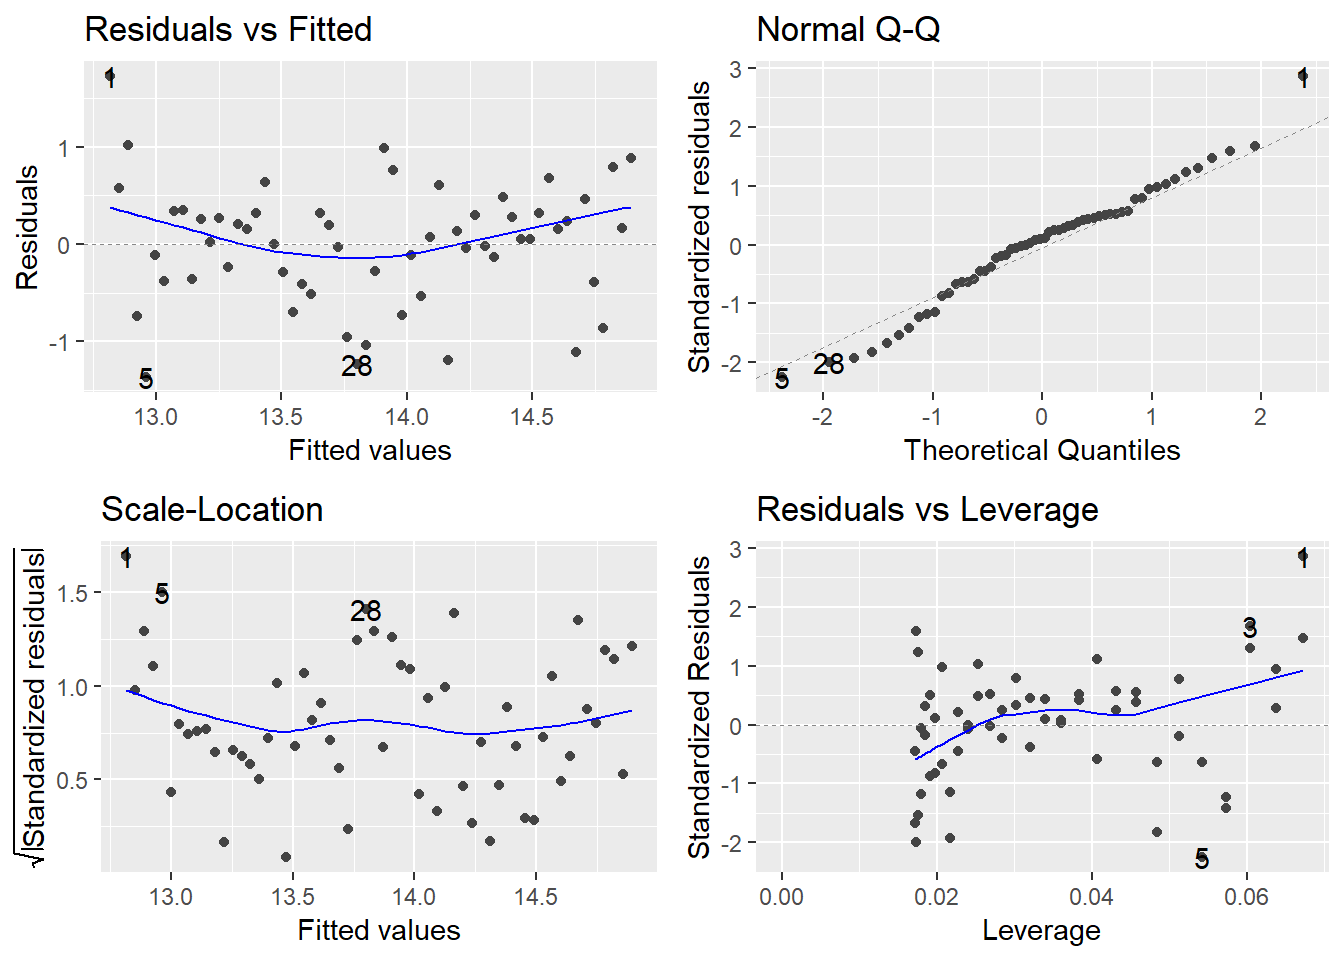
\includegraphics{Online_R_Course_files/figure-latex/unnamed-chunk-164-1.pdf}

Do these plots look OK? What are we actually looking for here?

In particular we can see a problem with the trend in the residual vs fitted plot as there is clear curvature in the pattern. Does this make sense if we go back to our original scatter plots and the loess models fitted by geom\_smooth

\hypertarget{updating-model}{%
\section{Updating Model}\label{updating-model}}

One solution to solve the problem we have might be to fit a model only on the years between 1975 to 2015, since the trend during this range appears to be relatively linear. We can filter our data and then pipe through to lm:

\begin{Shaded}
\begin{Highlighting}[]
\NormalTok{eastbourne }\OperatorTok
\StringTok{  }\KeywordTok{filter}\NormalTok{(yyyy}\OperatorTok{>=}\DecValTok{1975}\NormalTok{) }\OperatorTok
\StringTok{    }\KeywordTok{ggplot}\NormalTok{(}\KeywordTok{aes}\NormalTok{(}\DataTypeTok{y=}\NormalTok{tmax,}\DataTypeTok{x=}\NormalTok{yyyy))}\OperatorTok{+}
\StringTok{     }\KeywordTok{geom_point}\NormalTok{()}\OperatorTok{+}
\StringTok{       }\KeywordTok{geom_smooth}\NormalTok{(}\DataTypeTok{method=}\StringTok{"lm"}\NormalTok{)}
\end{Highlighting}
\end{Shaded}

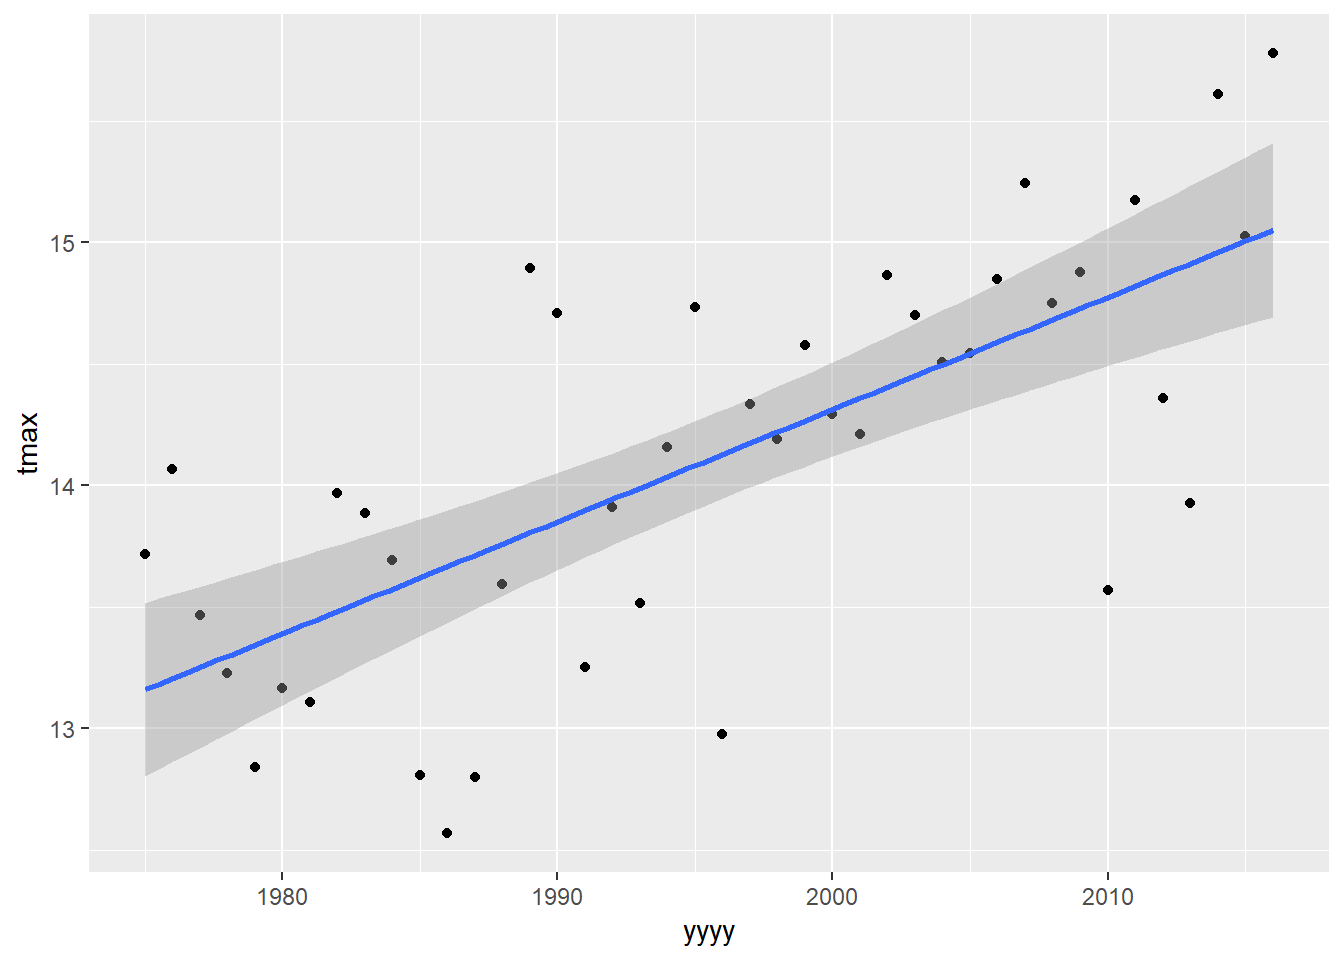
\includegraphics{Online_R_Course_files/figure-latex/unnamed-chunk-165-1.pdf}

\begin{Shaded}
\begin{Highlighting}[]
\NormalTok{eastbourne }\OperatorTok
\StringTok{  }\KeywordTok{filter}\NormalTok{(yyyy}\OperatorTok{>=}\DecValTok{1975}\NormalTok{) }\OperatorTok
\StringTok{    }\KeywordTok{lm}\NormalTok{(tmax}\OperatorTok{~}\NormalTok{yyyy,}\DataTypeTok{data=}\NormalTok{.)}
\end{Highlighting}
\end{Shaded}

\begin{verbatim}
## 
## Call:
## lm(formula = tmax ~ yyyy, data = .)
## 
## Coefficients:
## (Intercept)         yyyy  
##   -77.97949      0.04615
\end{verbatim}

This is slightly different to what we have seen previously with pipes because the first argument of lm() is the formula and not the data. Using the pipe automatically puts the data into the first argument of the next line. For lm(), and other functions where data is not the first argument, then saying ``data=.'' tells R where to put the data from the previous line.

Again we need to assign this to an object to do other useful things! Let's first check the model validity plots to see if they look any better:

\begin{Shaded}
\begin{Highlighting}[]
\NormalTok{tmaxmodel_}\DecValTok{1975}\NormalTok{<-}
\StringTok{  }\NormalTok{eastbourne }\OperatorTok
\StringTok{  }\KeywordTok{filter}\NormalTok{(yyyy}\OperatorTok{>=}\DecValTok{1975}\NormalTok{) }\OperatorTok
\StringTok{    }\KeywordTok{lm}\NormalTok{(tmax}\OperatorTok{~}\NormalTok{yyyy,}\DataTypeTok{data=}\NormalTok{.)}

\KeywordTok{autoplot}\NormalTok{(tmaxmodel_}\DecValTok{1975}\NormalTok{)}
\end{Highlighting}
\end{Shaded}

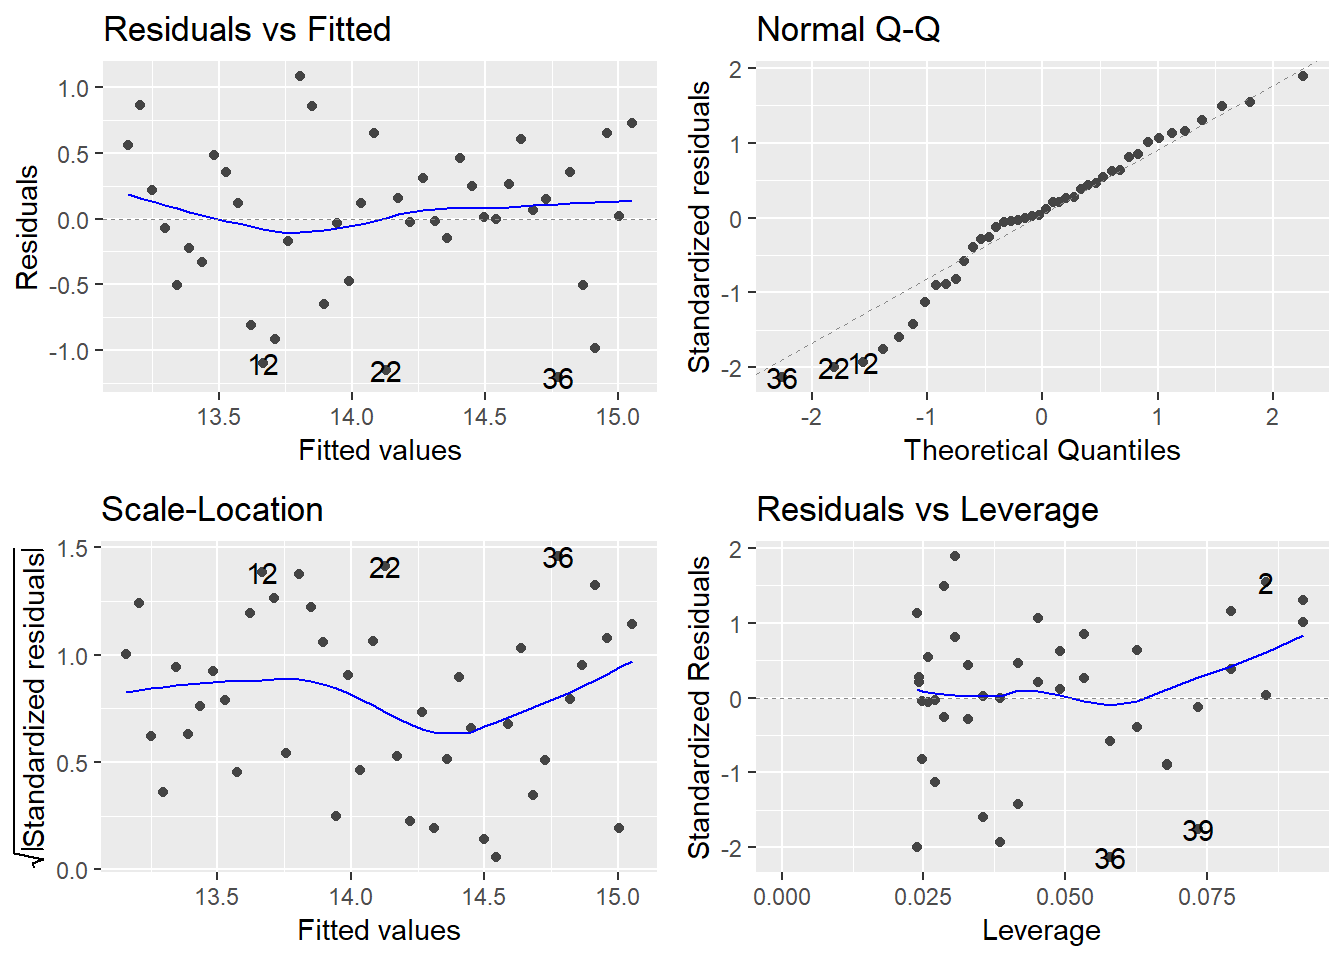
\includegraphics{Online_R_Course_files/figure-latex/unnamed-chunk-166-1.pdf}

This looks better. Let's take another look at these result:

\begin{Shaded}
\begin{Highlighting}[]
\KeywordTok{summary}\NormalTok{(tmaxmodel_}\DecValTok{1975}\NormalTok{)}
\end{Highlighting}
\end{Shaded}

\begin{verbatim}
## 
## Call:
## lm(formula = tmax ~ yyyy, data = .)
## 
## Residuals:
##      Min       1Q   Median       3Q      Max 
## -1.20748 -0.30145  0.04414  0.35503  1.08659 
## 
## Coefficients:
##               Estimate Std. Error t value Pr(>|t|)    
## (Intercept) -77.979495  14.810825  -5.265 5.07e-06 ***
## yyyy          0.046146   0.007422   6.217 2.34e-07 ***
## ---
## Signif. codes:  0 '***' 0.001 '**' 0.01 '*' 0.05 '.' 0.1 ' ' 1
## 
## Residual standard error: 0.583 on 40 degrees of freedom
## Multiple R-squared:  0.4915, Adjusted R-squared:  0.4788 
## F-statistic: 38.66 on 1 and 40 DF,  p-value: 2.337e-07
\end{verbatim}

\hypertarget{confidence-and-prediction-intervals}{%
\section{Confidence and Prediction Intervals}\label{confidence-and-prediction-intervals}}

The geom\_smooth function fits confidence intervals around the line. This tells us the margin of error in the expected value of temperature in each year.
This is OK, but it can also be very useful to include prediction intervals. This tells us the range where we would expect any individual observation to be.

The functions add\_ci and add\_pi can add in confidence intervals and prediction intervals to our original data. These work nicely in pipes, where we simply need the name of the model inside these functions.

\begin{Shaded}
\begin{Highlighting}[]
\NormalTok{eastbourne_int<-eastbourne }\OperatorTok
\StringTok{  }\KeywordTok{filter}\NormalTok{(yyyy}\OperatorTok{>=}\DecValTok{1975}\NormalTok{) }\OperatorTok
\StringTok{    }\KeywordTok{add_pi}\NormalTok{(tmaxmodel_}\DecValTok{1975}\NormalTok{) }\OperatorTok
\StringTok{      }\KeywordTok{add_ci}\NormalTok{(tmaxmodel_}\DecValTok{1975}\NormalTok{)}
\end{Highlighting}
\end{Shaded}

To add in errors as lines this needs the \texttt{geom\_ribbon} geom from ggplot2.

\begin{Shaded}
\begin{Highlighting}[]
\KeywordTok{ggplot}\NormalTok{(eastbourne_int,}\KeywordTok{aes}\NormalTok{(}\DataTypeTok{x=}\NormalTok{yyyy,}\DataTypeTok{y=}\NormalTok{tmax))}\OperatorTok{+}
\StringTok{ }\KeywordTok{geom_point}\NormalTok{() }\OperatorTok{+}
\StringTok{  }\KeywordTok{geom_smooth}\NormalTok{(}\DataTypeTok{method=}\StringTok{"lm"}\NormalTok{)}\OperatorTok{+}
\StringTok{   }\KeywordTok{geom_ribbon}\NormalTok{(}\KeywordTok{aes}\NormalTok{(}\DataTypeTok{ymax=}\NormalTok{UPB0}\FloatTok{.975}\NormalTok{,}\DataTypeTok{ymin=}\NormalTok{ LPB0}\FloatTok{.025}\NormalTok{)) }
\end{Highlighting}
\end{Shaded}

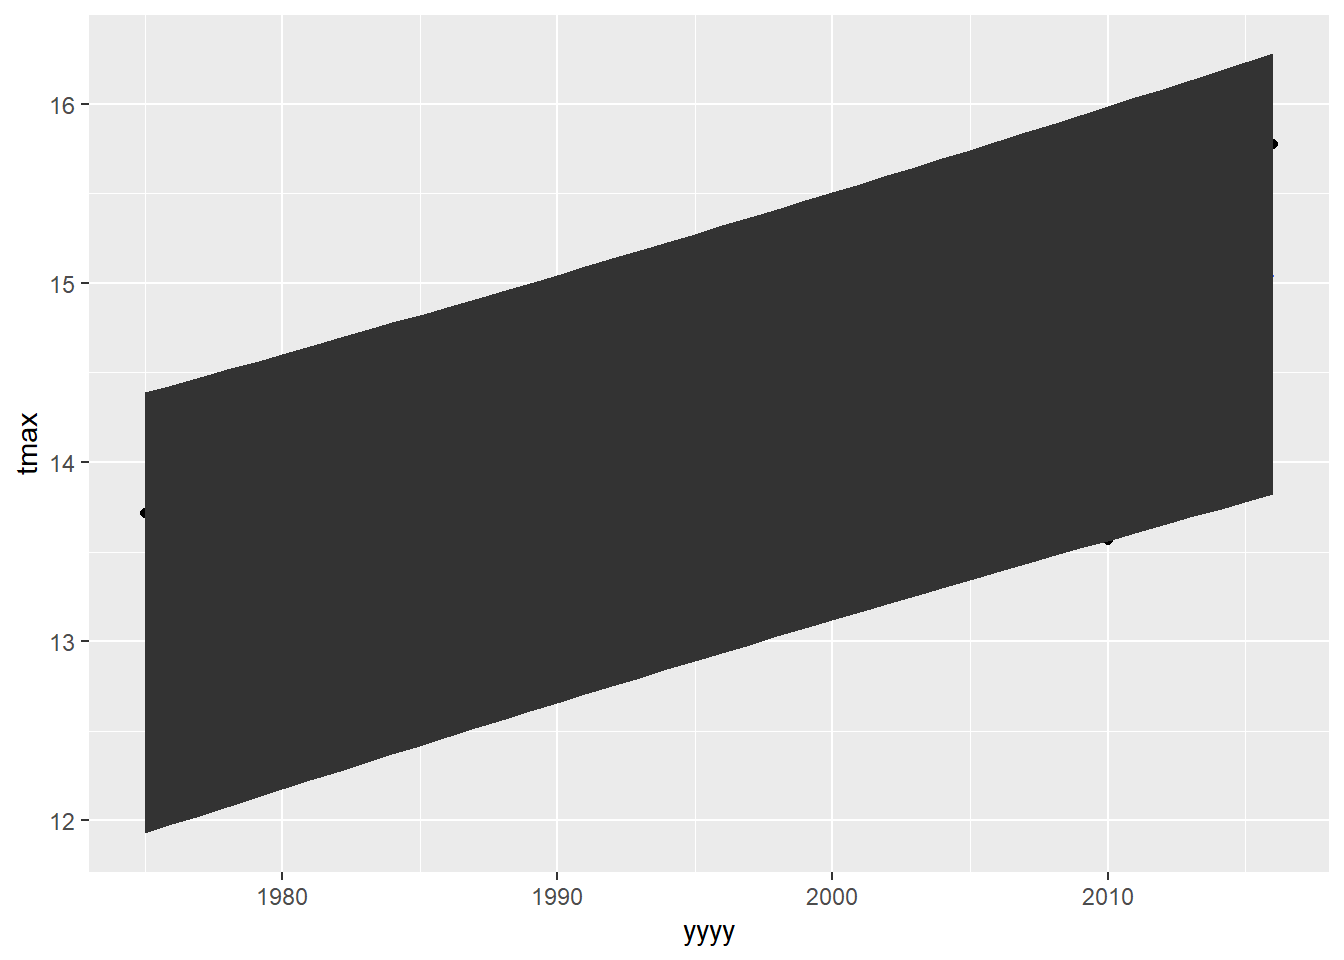
\includegraphics{Online_R_Course_files/figure-latex/unnamed-chunk-169-1.pdf}

\textbf{QUESTION - This graph is `correct', but looks horrible. Can you find the options to make this plot look a bit better? Instead of a big black blob, how can we have something more similar to the way the error bar gets plotted in geom\_smooth() - transparent and shaded in a colour rather than black?}

We can also use add\_ci or add\_pi to give us future predictions to extrapolate our model into the future

\begin{Shaded}
\begin{Highlighting}[]
\NormalTok{predictiondata<-}\KeywordTok{data.frame}\NormalTok{(}\DataTypeTok{yyyy=}\DecValTok{1975}\OperatorTok{:}\DecValTok{2100}\NormalTok{) }\OperatorTok
\StringTok{   }\KeywordTok{add_ci}\NormalTok{(tmaxmodel_}\DecValTok{1975}\NormalTok{) }\OperatorTok
\StringTok{     }\KeywordTok{add_pi}\NormalTok{(tmaxmodel_}\DecValTok{1975}\NormalTok{) }
\NormalTok{predictiondata}
\end{Highlighting}
\end{Shaded}

\begin{verbatim}
## # A tibble: 126 x 6
##     yyyy  pred LCB0.025 UCB0.975 LPB0.025 UPB0.975
##    <int> <dbl>    <dbl>    <dbl>    <dbl>    <dbl>
##  1  1975  13.2     12.8     13.5     11.9     14.4
##  2  1976  13.2     12.9     13.5     12.0     14.4
##  3  1977  13.3     12.9     13.6     12.0     14.5
##  4  1978  13.3     13.0     13.6     12.1     14.5
##  5  1979  13.3     13.0     13.7     12.1     14.6
##  6  1980  13.4     13.1     13.7     12.2     14.6
##  7  1981  13.4     13.2     13.7     12.2     14.6
##  8  1982  13.5     13.2     13.8     12.3     14.7
##  9  1983  13.5     13.3     13.8     12.3     14.7
## 10  1984  13.6     13.3     13.8     12.4     14.8
## # ... with 116 more rows
\end{verbatim}

We can plot our predicted model into the future onto a nice graph as well. But - we have our raw data in one file and our predicted data in another file. So we are going to show you how to use ggplot to make a single plot from multple data frames.

Using plot1 (saved earlier) - which had used the data=eastbourne.

\begin{Shaded}
\begin{Highlighting}[]
\NormalTok{plot1}
\end{Highlighting}
\end{Shaded}

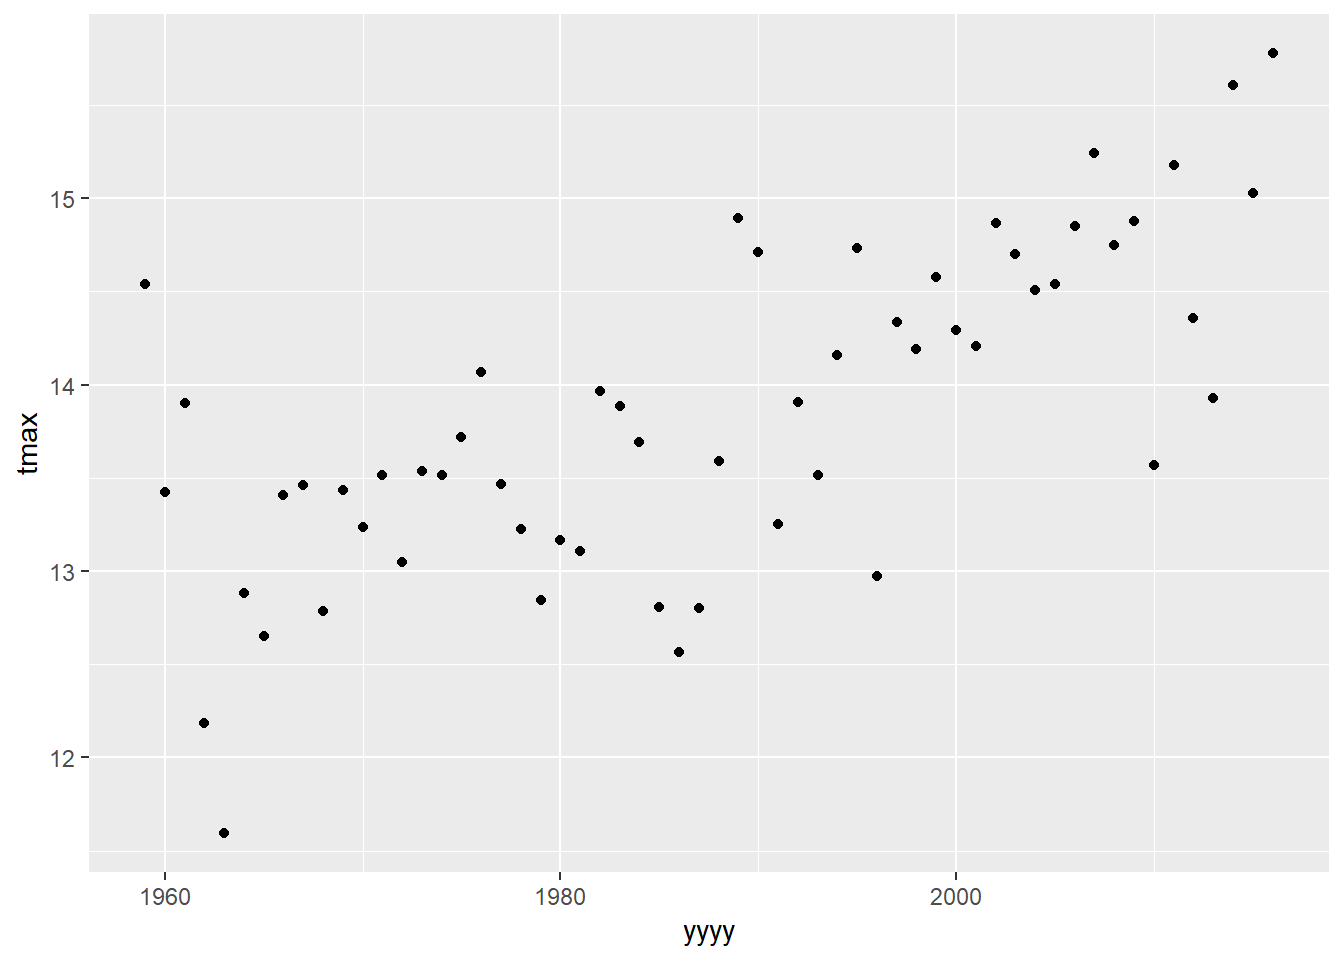
\includegraphics{Online_R_Course_files/figure-latex/unnamed-chunk-171-1.pdf}

We can add in the aesthetics and data into any geom. But we need to add in also an option inherit.aes=FALSE. This tells R to ignore the `global' aesthetics which were set in the original ggplot() statement.

\begin{Shaded}
\begin{Highlighting}[]
\NormalTok{plot1}\OperatorTok{+}
\StringTok{  }\KeywordTok{geom_line}\NormalTok{(}\KeywordTok{aes}\NormalTok{(}\DataTypeTok{x=}\NormalTok{yyyy,}\DataTypeTok{y=}\NormalTok{pred),}\DataTypeTok{data=}\NormalTok{predictiondata,}\DataTypeTok{inherit.aes =} \OtherTok{FALSE}\NormalTok{) }
\end{Highlighting}
\end{Shaded}

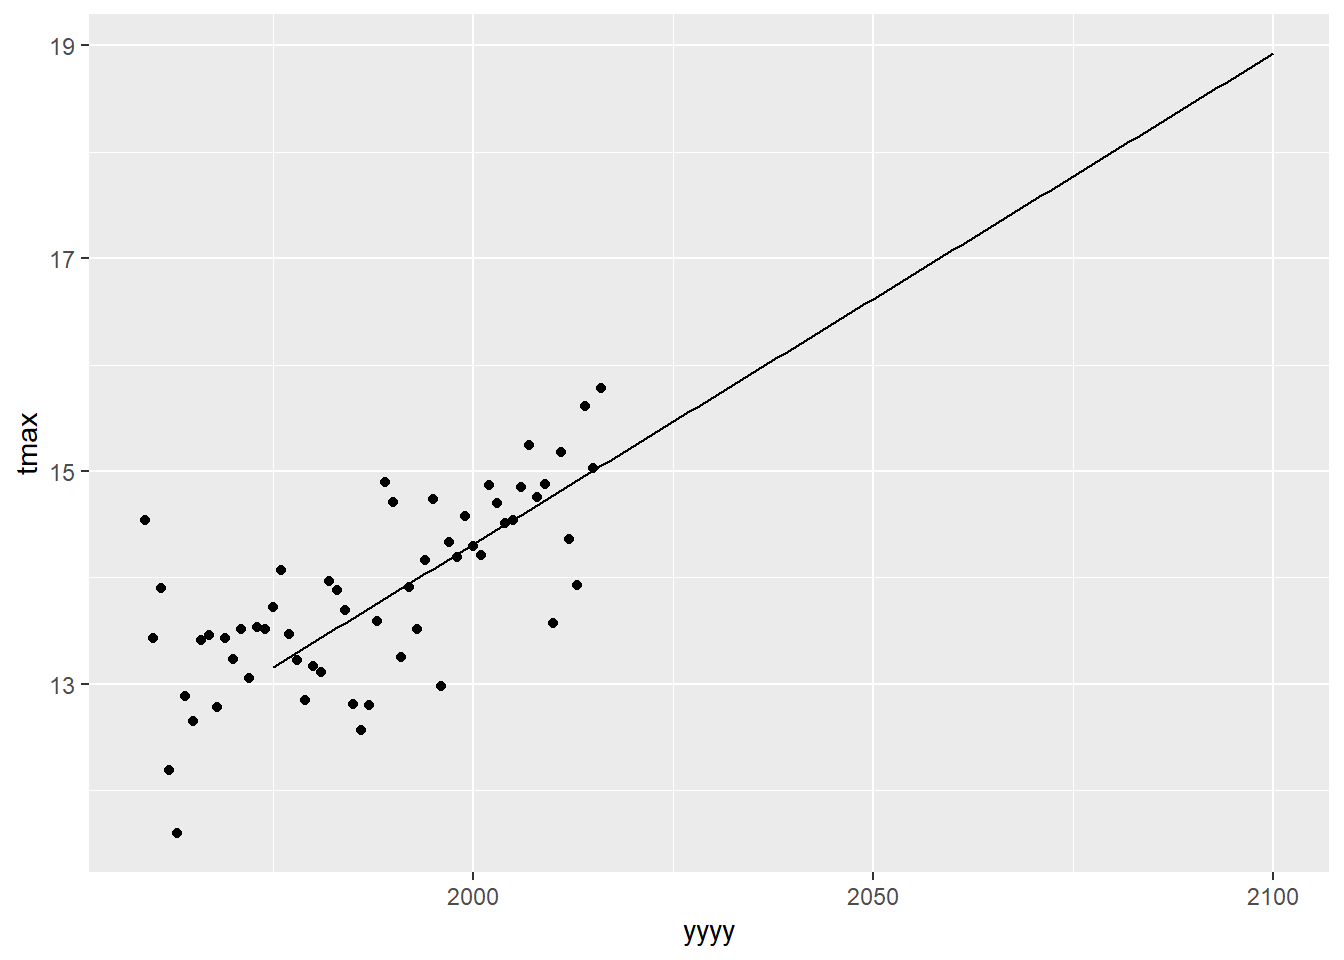
\includegraphics{Online_R_Course_files/figure-latex/unnamed-chunk-172-1.pdf}

We can then add our prediction interval in the same way:

\begin{Shaded}
\begin{Highlighting}[]
\NormalTok{plot1}\OperatorTok{+}
\StringTok{  }\KeywordTok{geom_line}\NormalTok{(}\KeywordTok{aes}\NormalTok{(}\DataTypeTok{x=}\NormalTok{yyyy,}\DataTypeTok{y=}\NormalTok{pred),}\DataTypeTok{data=}\NormalTok{predictiondata,}\DataTypeTok{inherit.aes =} \OtherTok{FALSE}\NormalTok{) }\OperatorTok{+}
\StringTok{    }\KeywordTok{geom_ribbon}\NormalTok{(}\KeywordTok{aes}\NormalTok{(}\DataTypeTok{x=}\NormalTok{yyyy,}\DataTypeTok{ymax=}\NormalTok{UPB0}\FloatTok{.975}\NormalTok{,}\DataTypeTok{ymin=}\NormalTok{LPB0}\FloatTok{.025}\NormalTok{),}\DataTypeTok{data=}\NormalTok{predictiondata,}\DataTypeTok{alpha=}\FloatTok{0.2}\NormalTok{,}\DataTypeTok{fill=}\StringTok{"red"}\NormalTok{,}\DataTypeTok{inherit.aes =} \OtherTok{FALSE}\NormalTok{)}
\end{Highlighting}
\end{Shaded}

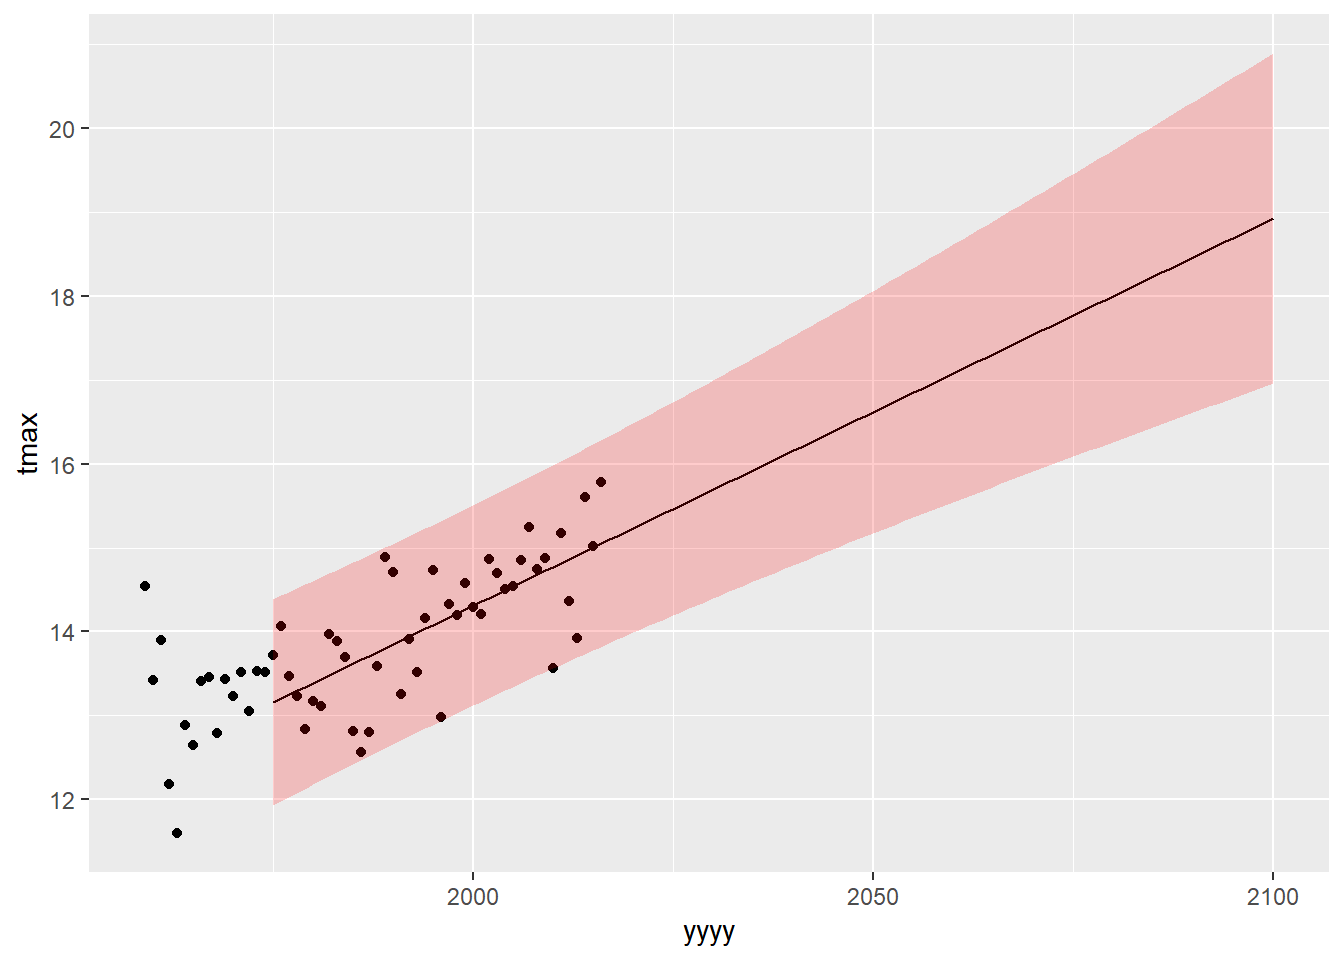
\includegraphics{Online_R_Course_files/figure-latex/unnamed-chunk-173-1.pdf}

\hypertarget{extending-to-multiple-regression}{%
\section{Extending to multiple regression:}\label{extending-to-multiple-regression}}

We can add variables into our model using +. Let's add rainfall as a potential predictor for tmax.

\begin{Shaded}
\begin{Highlighting}[]
\NormalTok{tmaxrain<-}\KeywordTok{lm}\NormalTok{(tmax}\OperatorTok{~}\NormalTok{yyyy}\OperatorTok{+}\NormalTok{rain,}\DataTypeTok{data=}\NormalTok{eastbourne)}
\KeywordTok{summary}\NormalTok{(tmaxrain)}
\end{Highlighting}
\end{Shaded}

\begin{verbatim}
## 
## Call:
## lm(formula = tmax ~ yyyy + rain, data = eastbourne)
## 
## Residuals:
##      Min       1Q   Median       3Q      Max 
## -1.36728 -0.37668  0.06186  0.31932  1.72483 
## 
## Coefficients:
##               Estimate Std. Error t value Pr(>|t|)    
## (Intercept) -5.850e+01  9.889e+00  -5.916 2.20e-07 ***
## yyyy         3.642e-02  4.950e-03   7.359 9.74e-10 ***
## rain        -5.395e-04  7.796e-03  -0.069    0.945    
## ---
## Signif. codes:  0 '***' 0.001 '**' 0.01 '*' 0.05 '.' 0.1 ' ' 1
## 
## Residual standard error: 0.6294 on 55 degrees of freedom
## Multiple R-squared:  0.4978, Adjusted R-squared:  0.4795 
## F-statistic: 27.26 on 2 and 55 DF,  p-value: 5.95e-09
\end{verbatim}

It looks like there is no evidence of a relationship between rainfall and maximum temperatures.

\hypertarget{exercise}{%
\section{Exercise}\label{exercise}}

Repeat the whole modelling process for the column tmin instead of tmax. Start by making a scatter plot, using geom\_smooth to fit a linear model onto this graph and then use lm() to fit a model, check the validity, draw conclusions about how tmin has changed over time, if so by how much, and make predictions for the next 5 years

\begin{itemize}
\tightlist
\item
  Start with producing a scatter plot, using geom\_smooth to fit lines, using booth the smoother and the linear regression
\end{itemize}

\begin{Shaded}
\begin{Highlighting}[]
\KeywordTok{ggplot}\NormalTok{(}\DataTypeTok{data=}\NormalTok{eastbourne,}\KeywordTok{aes}\NormalTok{(}\DataTypeTok{y=}\NormalTok{??,}\DataTypeTok{x=}\NormalTok{???))}\OperatorTok{+}\NormalTok{???}
\end{Highlighting}
\end{Shaded}

\begin{itemize}
\item
  Then fit a model of minimum temperature against year:
\item
  Then check the model validity:
\item
  Then look at and interpret the summary table:
\item
  Then make a plot showing the fitted model, and add some prediction intervals around your model:
\item
  (Difficult question) Make a plot showing both tmin and tmax on the same axes and the fitted models for both.
\end{itemize}

\hypertarget{simulation}{%
\chapter{Simulation}\label{simulation}}

\hypertarget{description-of-the-session-goal}{%
\section{Description of the session goal}\label{description-of-the-session-goal}}

In this session we will learn about:
\emph{Packages}\\
\emph{Sampling}\\
\emph{Functions}\\
\emph{Loops}\\
At the end we'll try to make a concrete use of all of it and answer an interesting question in probability.

Ready?

\hypertarget{find-and-install-r-packages}{%
\section{Find and install R packages}\label{find-and-install-r-packages}}

A nice website to find packages is \url{https://www.rdocumentation.org}\\
That's how I found about the package ``ukbabynames'' that contains data for all baby names given at least three times between 1996 and 2015.

To install a package called ``ukbabynames'', we do

\begin{Shaded}
\begin{Highlighting}[]
\KeywordTok{install.packages}\NormalTok{(}\StringTok{"ukbabynames"}\NormalTok{)}
\end{Highlighting}
\end{Shaded}

Once a package is installed in your computer, it will remain installed and so you only need to install the package again if you're updating your version of R.

However, each time you open a new session of R or Rstudio, you need to load the package if you want to use it:

\begin{Shaded}
\begin{Highlighting}[]
\KeywordTok{library}\NormalTok{(ukbabynames)}
\end{Highlighting}
\end{Shaded}

I'm sure you noticed that we've done it several times already with packages like \texttt{ggplot2} or \texttt{dplyr()}.

Most often we are interested in the functions of the packages we install, but a package can also contain datasets and in this case, the package ``ukbabynames'' contains a dataframe of the same name and this is what we will use from it:

\begin{Shaded}
\begin{Highlighting}[]
\KeywordTok{View}\NormalTok{(ukbabynames)}
\end{Highlighting}
\end{Shaded}

\textbf{QUESTION 2.1: The function \texttt{say()} from the package ``cowsay'' is useless, but funny. Install the package ``cowsay''. Then, when the installation is finished (you have a to wait a bit, like for any package you would install), load the package and try to run the command \texttt{say(Hello\ R!)}. What happens?}

\begin{Shaded}
\begin{Highlighting}[]
\NormalTok{???.???(}\StringTok{"cowsay"}\NormalTok{)}
\end{Highlighting}
\end{Shaded}

\begin{Shaded}
\begin{Highlighting}[]
\NormalTok{???(cowsay)}
\KeywordTok{say}\NormalTok{(}\StringTok{"Hello R!"}\NormalTok{)}
\end{Highlighting}
\end{Shaded}

\hypertarget{sampling-from-data-or-known-distributions}{%
\section{Sampling from data or known distributions}\label{sampling-from-data-or-known-distributions}}

\hypertarget{sampling-from-data}{%
\section{Sampling from data}\label{sampling-from-data}}

The \texttt{sample()} function allows you to choose a random sample from a list of values.

\begin{Shaded}
\begin{Highlighting}[]
\KeywordTok{sample}\NormalTok{(}\DecValTok{1}\OperatorTok{:}\DecValTok{30}\NormalTok{, }\DecValTok{5}\NormalTok{)}
\end{Highlighting}
\end{Shaded}

\begin{verbatim}
## [1] 18  9 29 17  1
\end{verbatim}

The first argument is the values to sample from and the second is the number of values to sample. If we omit the second argument, we get all the values, but in a random order:

\begin{Shaded}
\begin{Highlighting}[]
\KeywordTok{sample}\NormalTok{(}\DecValTok{1}\OperatorTok{:}\DecValTok{12}\NormalTok{)}
\end{Highlighting}
\end{Shaded}

\begin{verbatim}
##  [1]  7  3 10  8  2  4 12  9  5 11  6  1
\end{verbatim}

By default \texttt{sample()} samples without replacement, so when you do

\begin{Shaded}
\begin{Highlighting}[]
\KeywordTok{sample}\NormalTok{(}\DecValTok{1}\OperatorTok{:}\DecValTok{5}\NormalTok{, }\DecValTok{10}\NormalTok{)}
\end{Highlighting}
\end{Shaded}

You get an error. To sample with replacement you need to add the argument replace=TRUE:

\begin{Shaded}
\begin{Highlighting}[]
\KeywordTok{sample}\NormalTok{(}\DecValTok{1}\OperatorTok{:}\DecValTok{5}\NormalTok{, }\DecValTok{10}\NormalTok{, }\DataTypeTok{replace=}\OtherTok{TRUE}\NormalTok{)}
\end{Highlighting}
\end{Shaded}

\begin{verbatim}
##  [1] 3 5 3 5 2 3 4 5 5 2
\end{verbatim}

\hypertarget{generating-random-numbers-from-distributions}{%
\section{Generating random numbers from distributions}\label{generating-random-numbers-from-distributions}}

We can also generate random numbers from known distribution.

runif (uniform)\\
rpois (poisson)\\
rnorm (normal)\\
rbinom (binomial)\\
rgamma (gamma)\\
rbeta (beta)

The first argument for all of these is n, the number of samples to generate. Following arguments can specify parameters for the distribution.

Here are three random numbers coming from a standard normal distribution:

\begin{Shaded}
\begin{Highlighting}[]
\KeywordTok{rnorm}\NormalTok{(}\DecValTok{3}\NormalTok{)}
\end{Highlighting}
\end{Shaded}

\begin{verbatim}
## [1]  0.1005724 -0.4920847  0.1394214
\end{verbatim}

here, six random numbers coming from a normal distribution with mean 5 and standard deviation 2:

\begin{Shaded}
\begin{Highlighting}[]
\KeywordTok{rnorm}\NormalTok{(}\DecValTok{6}\NormalTok{, }\DecValTok{5}\NormalTok{, }\DecValTok{2}\NormalTok{)}
\end{Highlighting}
\end{Shaded}

\begin{verbatim}
## [1]  3.943484  5.508093  5.707986 11.513517  6.817776  2.529775
\end{verbatim}

And here is 5 random numbers coming from a uniform distribution between 0 and 1:

\begin{Shaded}
\begin{Highlighting}[]
\KeywordTok{runif}\NormalTok{(}\DecValTok{5}\NormalTok{)}
\end{Highlighting}
\end{Shaded}

\begin{verbatim}
## [1] 0.3346454 0.4547205 0.2853403 0.5616378 0.3075359
\end{verbatim}

\hypertarget{reproducing-samples}{%
\section{Reproducing samples}\label{reproducing-samples}}

Note that if you run any of these commands again you'll get a different sample. Sometimes you want your random sample to be reproducible i.e.~you want to get the same random sample each time you run the script.\\
This is possible because the generation of randomness of any programming language is based on some algorithm that takes some ``seed'' number as input. It is usually based on the internal clock of your computer and so it changes all the time. But we can fix the seed manually by running the function \texttt{set.seed()} with an integer inside the parenthesis

\textbf{QUESTION 3.1: Produce 5 random integers between 1 and 20, without replacement. Set a seed before sampling and confirm that you get the same sample each time you run it.}

\begin{Shaded}
\begin{Highlighting}[]
\NormalTok{???}
\KeywordTok{sample}\NormalTok{(???, ???)}
\end{Highlighting}
\end{Shaded}

\hypertarget{sampling-from-data-1}{%
\section{Sampling from data}\label{sampling-from-data-1}}

We can sample from data in the same way as above. Here I am sampling 10 random names from the ukbabynames dataframe:

\begin{Shaded}
\begin{Highlighting}[]
\KeywordTok{sample}\NormalTok{(ukbabynames}\OperatorTok{$}\NormalTok{name, }\DecValTok{10}\NormalTok{)}
\end{Highlighting}
\end{Shaded}

\begin{verbatim}
##  [1] "Amisha"  "Abubakr" "Craig"   "Eirian"  "Aashir"  "Fisher"  "Melika" 
##  [8] "Reza"    "Aleasha" "Phil"
\end{verbatim}

Note also that the package dplyr contains its own functon sample\_n() that allow you to sample the number of rows that you indicate as its second argument (which is the first argument if you use ``\%\textgreater{}\%''):

\begin{Shaded}
\begin{Highlighting}[]
\KeywordTok{library}\NormalTok{(dplyr)}
\NormalTok{ukbabynames }\OperatorTok\StringTok{ }\KeywordTok{sample_n}\NormalTok{(}\DecValTok{8}\NormalTok{)}
\end{Highlighting}
\end{Shaded}

\begin{verbatim}
##   year sex     name  n rank
## 1 1998   F   Briege  3 3848
## 2 1998   M    Caner  8 1485
## 3 2004   M  Fardeen 13 1347
## 4 2006   F   Kassia  9 2320
## 5 2001   M   Tyreke  7 1746
## 6 2011   F    Kiswa  3 5785
## 7 2005   M    Nasif  5 2754
## 8 2000   F Annalisa  8 1995
\end{verbatim}

\hypertarget{making-functions}{%
\section{Making functions}\label{making-functions}}

\hypertarget{when-to-write-your-own-functions}{%
\section{When to write your own functions}\label{when-to-write-your-own-functions}}

If there's already a function in R that does what you want then writing it yourself will almost definitely be less efficient as well as wasting your time. For example, writing a function to calculate the standard deviation of a column is not needed since there is already the \texttt{sd()} function.

Many common things will already have function either in base R or a package, however if you find yourself doing the same specific task multiple times, writing your own function can save you copying and pasting code and this is always desirable.

We define a function that way:

\begin{Shaded}
\begin{Highlighting}[]
\NormalTok{myFunction <-}\StringTok{ }\ControlFlowTok{function}\NormalTok{()\{}
  
\NormalTok{\}}
\end{Highlighting}
\end{Shaded}

and use it like any other function

\begin{Shaded}
\begin{Highlighting}[]
\KeywordTok{myFunction}\NormalTok{()}
\end{Highlighting}
\end{Shaded}

\begin{verbatim}
## NULL
\end{verbatim}

Yes for now our function doesn't do anything, because there is nothing inside the brakets (note tha they are curly brackets by the way, not normal or square brackets!).

We can make the function return something, with the function return()

\begin{Shaded}
\begin{Highlighting}[]
\NormalTok{myFunction <-}\StringTok{ }\ControlFlowTok{function}\NormalTok{()\{}
  \KeywordTok{return}\NormalTok{(}\DecValTok{2}\NormalTok{)}
\NormalTok{\}}
\KeywordTok{myFunction}\NormalTok{()}
\end{Highlighting}
\end{Shaded}

\begin{verbatim}
## [1] 2
\end{verbatim}

Our function just returns two each time we call it. What an awesome function!!!

Let's put inside some code that generates the sum of 3 uniformely distributed random numbers and let's return that sum

\begin{Shaded}
\begin{Highlighting}[]
\NormalTok{myFunction <-}\StringTok{ }\ControlFlowTok{function}\NormalTok{()\{}
\NormalTok{  few_runif <-}\StringTok{ }\KeywordTok{runif}\NormalTok{(}\DecValTok{3}\NormalTok{)}
\NormalTok{  sum_few_runif <-}\StringTok{ }\KeywordTok{sum}\NormalTok{(few_runif)}
  \KeywordTok{return}\NormalTok{(sum_few_runif)}
\NormalTok{\}}
\KeywordTok{myFunction}\NormalTok{()}
\end{Highlighting}
\end{Shaded}

\begin{verbatim}
## [1] 2.253677
\end{verbatim}

Yayy! Did you see that each time you run it you get a different number?

\textbf{QUESTION 4.1: Create a function called myFunctionNorm that would return the sum of 5 normally distributed random numbers. Run it to see if it works}

\begin{Shaded}
\begin{Highlighting}[]
\NormalTok{??? <-}\StringTok{ }\ControlFlowTok{function}\NormalTok{()\{}
\NormalTok{  few_rnorm <-}\StringTok{ }\NormalTok{???(???)}
\NormalTok{  sum_few_rnorm <-}\StringTok{ }\NormalTok{???(???)}
  \KeywordTok{return}\NormalTok{(???)}
\NormalTok{\}}

\NormalTok{???()}
\end{Highlighting}
\end{Shaded}

You may be tempted to put a number inside the parenthesis. Would myFunction(5) generate 5 random numbers?

\begin{Shaded}
\begin{Highlighting}[]
\KeywordTok{myFunction}\NormalTok{(}\DecValTok{5}\NormalTok{)}
\end{Highlighting}
\end{Shaded}

Argh, no, because we didn't define what the function should do with what is inside the parenthesis.

We can generate more than one number with the function replicate() though, which simply runs what we put as its second argument (second thing inside the parentheses), the number of times we indicate as its first argument:

\begin{Shaded}
\begin{Highlighting}[]
\NormalTok{randomNumbers <-}\StringTok{ }\KeywordTok{replicate}\NormalTok{(}\DecValTok{5}\NormalTok{, }\KeywordTok{myFunction}\NormalTok{())}
\NormalTok{randomNumbers}
\end{Highlighting}
\end{Shaded}

\begin{verbatim}
## [1] 1.6814483 0.8994199 1.0328035 1.5335543 0.5780411
\end{verbatim}

If we felt that the command replicate(number, myFunction()) was a bit too long to write, we could make a function similar to rnorm(), runif() etc. that gives the size of the sample as the first argument:

\begin{Shaded}
\begin{Highlighting}[]
\NormalTok{rsum3unif <-}\StringTok{ }\ControlFlowTok{function}\NormalTok{(n)\{}
\NormalTok{  some_sum3unif <-}\StringTok{ }\KeywordTok{replicate}\NormalTok{(n,}\KeywordTok{myFunction}\NormalTok{())}
  \KeywordTok{return}\NormalTok{(some_sum3unif)}
\NormalTok{\}}

\KeywordTok{rsum3unif}\NormalTok{(}\DecValTok{8}\NormalTok{)}
\end{Highlighting}
\end{Shaded}

\begin{verbatim}
## [1] 1.6704208 1.1739316 0.9551181 1.5962373 1.8420413 1.7429733 1.5424678
## [8] 1.7029722
\end{verbatim}

And here it is, we made a function that takes a number as its first (and only) argument, which it then used as the first argument of the function replicate, to generate the required number of random numbers (made from the sum of 3 uniformely distributed reandom numbers).

\textbf{QUESTION 4.2: the function below is supposed to print in the console a smiley that says the words given as its argument. What would you need to write in place of ??? for it to work? (note: the function cat() prints what's inside its parenthesis on the screen. ``\textbackslash{}\textbackslash{}n'' tells R to go to the next line). Try it}

\begin{Shaded}
\begin{Highlighting}[]
\NormalTok{smileysay <-}\StringTok{ }\ControlFlowTok{function}\NormalTok{(???)\{}
  \KeywordTok{cat}\NormalTok{(}\StringTok{"----------}\CharTok{\textbackslash{}n}\StringTok{"}\NormalTok{)}
  \KeywordTok{cat}\NormalTok{(words)}
  \KeywordTok{cat}\NormalTok{(}\StringTok{"}\CharTok{\textbackslash{}n}\StringTok{----------"}\NormalTok{)}
  \KeywordTok{cat}\NormalTok{(}\StringTok{"}\CharTok{\textbackslash{}n}\StringTok{       "}\NormalTok{)}
  \KeywordTok{cat}\NormalTok{(}\StringTok{"}\CharTok{\textbackslash{}n}\StringTok{ ^   ^ "}\NormalTok{)}
  \KeywordTok{cat}\NormalTok{(}\StringTok{"}\CharTok{\textbackslash{}n}\StringTok{   |   "}\NormalTok{)}
  \KeywordTok{cat}\NormalTok{(}\StringTok{"}\CharTok{\textbackslash{}n}\StringTok{  ___  "}\NormalTok{)}
  \KeywordTok{cat}\NormalTok{(}\StringTok{"}\CharTok{\textbackslash{}n}\StringTok{ |   | "}\NormalTok{)}
  \KeywordTok{cat}\NormalTok{(}\StringTok{"}\CharTok{\textbackslash{}n}\StringTok{  ---  "}\NormalTok{)}
\NormalTok{\}}

\KeywordTok{smileysay}\NormalTok{(}\StringTok{"Hello R!"}\NormalTok{)}
\end{Highlighting}
\end{Shaded}

\hypertarget{iterations-loops}{%
\section{Iterations (loops)}\label{iterations-loops}}

Here is a simple loop for:

\begin{Shaded}
\begin{Highlighting}[]
\ControlFlowTok{for}\NormalTok{(i }\ControlFlowTok{in} \DecValTok{3}\OperatorTok{:}\DecValTok{9}\NormalTok{) \{}
  \KeywordTok{print}\NormalTok{(i)}
\NormalTok{\}}
\end{Highlighting}
\end{Shaded}

\begin{verbatim}
## [1] 3
## [1] 4
## [1] 5
## [1] 6
## [1] 7
## [1] 8
## [1] 9
\end{verbatim}

The first part: (i in 3:9) provides the set of values to loop over. What is inside the curly brackets are the things that we are asking R to do at each iteration of the loop. Here we are asking to print i.

So we can read the above code as ``i will iteratively take all the values from 3 to 9 and for each iteration i should be printed on the screen''.

Instead of 3:9 we could put any kind of list of elements, and we don't need i to be called i. For example let's loop over a list of 10 random numbers, with the iteration variable called rnumber instead of i:

\begin{Shaded}
\begin{Highlighting}[]
\NormalTok{randomNumbers<-}\StringTok{ }\KeywordTok{runif}\NormalTok{(}\DecValTok{10}\NormalTok{)}
\ControlFlowTok{for}\NormalTok{(rnumber }\ControlFlowTok{in}\NormalTok{ randomNumbers) \{}
  \KeywordTok{print}\NormalTok{(rnumber)}
\NormalTok{\}}
\end{Highlighting}
\end{Shaded}

\begin{verbatim}
## [1] 0.150905
## [1] 0.07981697
## [1] 0.7518809
## [1] 0.6252572
## [1] 0.3606134
## [1] 0.6199747
## [1] 0.9494314
## [1] 0.5214505
## [1] 0.715805
## [1] 0.5418952
\end{verbatim}

\textbf{QUESTION 5.1: Make a loop with 12 iterations that generates and print at each iteration a random number coming from a standard normal distribution . Call the iteration variable ``iter''.}

\begin{Shaded}
\begin{Highlighting}[]
\ControlFlowTok{for}\NormalTok{(??? }\ControlFlowTok{in} \DecValTok{1}\OperatorTok{:}\NormalTok{???) \{}
\NormalTok{  random_number <-}\StringTok{ }\NormalTok{???(}\DecValTok{1}\NormalTok{)}
  \KeywordTok{print}\NormalTok{(???)}
\NormalTok{\}}
\end{Highlighting}
\end{Shaded}

In addition to being able to make loops, we will need to know how to check whether the name found in a box is or not the the name of the prisoner. We will do that with the function if()

If() works like the function for(), but is a bit simpler: if what is inside the parenthesis is true, then what is inside the curly brackets is performed. Let's generate a random number and check if it is larger than 0:

\begin{Shaded}
\begin{Highlighting}[]
\NormalTok{aNummber <-}\StringTok{ }\KeywordTok{rnorm}\NormalTok{(}\DecValTok{1}\NormalTok{)}
\NormalTok{aNummber}
\end{Highlighting}
\end{Shaded}

\begin{verbatim}
## [1] -1.433584
\end{verbatim}

\begin{Shaded}
\begin{Highlighting}[]
\ControlFlowTok{if}\NormalTok{(aNummber}\OperatorTok{>}\DecValTok{0}\NormalTok{) \{}
  \KeywordTok{print}\NormalTok{(}\StringTok{"it is larger than 0"}\NormalTok{)}
\NormalTok{\}}
\end{Highlighting}
\end{Shaded}

If you run the above code multiple times, you will see that sometimes something will be printed and sometimes not.

We can also ask R to perform an action when the condition inside the parenthesis is false, using the else command:

\begin{Shaded}
\begin{Highlighting}[]
\NormalTok{aNummber <-}\StringTok{ }\KeywordTok{rnorm}\NormalTok{(}\DecValTok{1}\NormalTok{)}
\NormalTok{aNummber}
\end{Highlighting}
\end{Shaded}

\begin{verbatim}
## [1] 2.441561
\end{verbatim}

\begin{Shaded}
\begin{Highlighting}[]
\ControlFlowTok{if}\NormalTok{(aNummber}\OperatorTok{>}\DecValTok{0}\NormalTok{) \{}
  \KeywordTok{print}\NormalTok{(}\StringTok{"it is larger than 0"}\NormalTok{)}
\NormalTok{\} }\ControlFlowTok{else}\NormalTok{\{}
  \KeywordTok{print}\NormalTok{(}\StringTok{"it is negative!"}\NormalTok{)}
\NormalTok{\}}
\end{Highlighting}
\end{Shaded}

\begin{verbatim}
## [1] "it is larger than 0"
\end{verbatim}

Also note that there exists another function called ``ifelse()'' that allows us to check a same condition on multiple elements at the same time. It works more like a normal function, the first argument being the condition to check, the second is what the function must return if the condition is checked and the third, what it must return if it is not. Let's generate 10 random numbers, check whether they are greater than 0, and for each of them, return 1 if this condtion is true and 0 if it is not:

\begin{Shaded}
\begin{Highlighting}[]
\NormalTok{fewNummbers <-}\StringTok{ }\KeywordTok{rnorm}\NormalTok{(}\DecValTok{10}\NormalTok{)}
\NormalTok{fewNummbers}
\end{Highlighting}
\end{Shaded}

\begin{verbatim}
##  [1] -1.0278143 -0.5947616  1.7244637  0.8588215 -0.1388179  0.2179455
##  [7] -0.1130976  1.1966227  0.3479995  0.4829627
\end{verbatim}

\begin{Shaded}
\begin{Highlighting}[]
\KeywordTok{ifelse}\NormalTok{(fewNummbers}\OperatorTok{>}\DecValTok{0}\NormalTok{, }\DecValTok{1}\NormalTok{, }\DecValTok{0}\NormalTok{)}
\end{Highlighting}
\end{Shaded}

\begin{verbatim}
##  [1] 0 0 1 1 0 1 0 1 1 1
\end{verbatim}

Do you see that you could achieve the same thing by looping over the 10 random number? Actually, R contains lots of functions like ifelse() that we could replace with loops but these functions are optimize and therefore much faster than using loops. Very often you'll be able to avoid using loops, and you should try so. They will only be unavoidable in some very specific situations.

\textbf{QUESTION 5.2: can you produce the same sequence of 0 and 1 as above, but using a loop for() and the if() function?}

\begin{Shaded}
\begin{Highlighting}[]
\ControlFlowTok{for}\NormalTok{(i }\ControlFlowTok{in}\NormalTok{ ???)\{}
  \ControlFlowTok{if}\NormalTok{(???)\{}
    \KeywordTok{print}\NormalTok{(???)}
\NormalTok{  \}}
  \ControlFlowTok{else}\NormalTok{\{}
    \KeywordTok{print}\NormalTok{(???)}
\NormalTok{  \}}
\NormalTok{\}}
\end{Highlighting}
\end{Shaded}

\hypertarget{puttng-it-all-together}{%
\section{Puttng it all together}\label{puttng-it-all-together}}

Here is a version of a very hard probability problem, with a very unintuitive result, that was first published by Peter Bro Miltersen and Anna Gal in the Proceedings of the 30th International Colloquium on Automata, Languages and Programming (ICALP):

The names of 100 prisoners are placed in 100 wooden boxes, one name to a box, and the boxes are lined up and numbered on a table in a room.
One by one, the prisoners are led into the room; each may look in at most 50 boxes, but must leave the room exactly as he found it and is permitted no further communication with the others.
The prisoners have a chance to plot their strategy in advance, and they are going to need it, because unless every single prisoner finds his own name all will subsequently be executed.

\textbf{QUESTION Can you guess what is the probability of success of the best strategy?}

One simple strategy would be for each prisoner to open 50 boxes at random. Since there are 100 boxes in total, each prisoner will have a probability of 1/2 to open the box that contains his name. Since each prisoner chooses randomly, the probability of success of the prisoners are independant and so the probability that all the prisoners will manage to open the box that contains their name is:

\begin{Shaded}
\begin{Highlighting}[]
\NormalTok{(}\DecValTok{1}\OperatorTok{/}\DecValTok{2}\NormalTok{)}\OperatorTok{^}\DecValTok{100}
\end{Highlighting}
\end{Shaded}

\begin{verbatim}
## [1] 7.888609e-31
\end{verbatim}

\ldots{} quite low!

Now the best strategy is quite simple, but understanding why it is the best is not at all obvious. It requires quite heavy math thinking about permutations and cycles. The same goes for calculating the associated probability of success. What we can do though is make some simulations to get an approximation of it.

The best strategy is the following:
First, the prisoners should agree on a random assignment of each box to a prisoner's name. We can imagine they all have in mind an imaginary common labelling of the 100 boxes.

Then each prisoner opens the box assigned to him. If the box contains his name, great. Otherwise, he opens the box labelled with the name found in this first box, and then he opens the box labelled with the name found in the second box etc. until he has either found his name, or opened 50 boxes.

\hypertarget{simulation-of-the-best-strategy}{%
\section{Simulation of the best strategy}\label{simulation-of-the-best-strategy}}

First, we need 100 names for our prisoners though. Here they are:

\begin{Shaded}
\begin{Highlighting}[]
\KeywordTok{set.seed}\NormalTok{(}\DecValTok{79}\NormalTok{)}
\NormalTok{list_prisoners <-}\StringTok{ }\KeywordTok{sample}\NormalTok{(ukbabynames}\OperatorTok{$}\NormalTok{name, }\DecValTok{100}\NormalTok{)}
\NormalTok{list_prisoners}
\end{Highlighting}
\end{Shaded}

\begin{verbatim}
##   [1] "Abela"       "Taher"       "Fynlay"      "Gisele"      "Wania"      
##   [6] "Adelaide"    "Mansoor"     "Larissa"     "Hayley"      "Iona"       
##  [11] "Anesh"       "Ashir"       "Luisa"       "Shakti"      "Scarlett"   
##  [16] "Evie"        "Tiger"       "Geoffrey"    "Cassie"      "Shariq"     
##  [21] "Alarna"      "Rawdah"      "Hadassah"    "Ikram"       "Amia"       
##  [26] "Jamieleigh"  "Demilade"    "Kovan"       "Demi-Rae"    "Azim"       
##  [31] "Gaurav"      "Christos"    "Jarin"       "Domenico"    "Manaal"     
##  [36] "Elijah"      "Katie-Mae"   "Abdulhakeem" "Krystal"     "Nana"       
##  [41] "Stacie"      "Yaw"         "Kay"         "Lily-Ann"    "Sola"       
##  [46] "Iara"        "Honie"       "Liana"       "George"      "Kaylem"     
##  [51] "Khushal"     "Bushra"      "Yasa"        "Filipa"      "Braidon"    
##  [56] "Lois"        "Daisy-may"   "Esmay"       "Alisdair"    "Sunaina"    
##  [61] "Muhanad"     "Huw"         "Taegan"      "Catelynn"    "Byron"      
##  [66] "Gage"        "Delphi"      "Faiz"        "Shaam"       "Zafir"      
##  [71] "Rivaan"      "Haajira"     "Amye"        "Warrick"     "Sajan"      
##  [76] "Ephraim"     "Evie-Lea"    "Ayush"       "Maisie"      "Ugochi"     
##  [81] "Samad"       "Bhavika"     "Delara"      "Monet"       "Kalani"     
##  [86] "Aashi"       "Hajira"      "Ishika"      "Isra"        "Kerensa"    
##  [91] "Samy"        "Mariam"      "Tinotenda"   "Shiloh"      "Glory"      
##  [96] "Diego"       "Dayton"      "Jeorgie"     "Promise"     "Payal"
\end{verbatim}

What we will need to do then is sample from this list to randomly place the names of the prisoners in the boxes:

\begin{Shaded}
\begin{Highlighting}[]
\NormalTok{name_inside_box <-}\StringTok{ }\KeywordTok{sample}\NormalTok{(list_prisoners)}
\NormalTok{name_inside_box[}\DecValTok{1}\OperatorTok{:}\DecValTok{10}\NormalTok{]}
\end{Highlighting}
\end{Shaded}

\begin{verbatim}
##  [1] "Gaurav"   "Jeorgie"  "Ashir"    "Bhavika"  "Dayton"   "Azim"    
##  [7] "Jarin"    "Amia"     "Hadassah" "Stacie"
\end{verbatim}

So for this simulation, in the first box there is the name \texttt{name\_inside\_box{[}1{]}}, in the second one, \texttt{name\_inside\_box{[}2{]}} etc.

And we can do the same to simulate the imaginary random labelling of the boxes by the prisoners when they develop their strategy:

\begin{Shaded}
\begin{Highlighting}[]
\NormalTok{label_on_box <-}\StringTok{ }\KeywordTok{sample}\NormalTok{(list_prisoners)}
\NormalTok{label_on_box[}\DecValTok{1}\OperatorTok{:}\DecValTok{10}\NormalTok{]}
\end{Highlighting}
\end{Shaded}

\begin{verbatim}
##  [1] "Haajira"  "Ishika"   "Lily-Ann" "Delara"   "Ashir"    "Kerensa" 
##  [7] "Demilade" "Tiger"    "Bhavika"  "Evie"
\end{verbatim}

And so \texttt{label\_on\_box{[}1{]}} will open the first box, where he will find the name \texttt{name\_inside\_box{[}1{]}}, which is not his own name, so he will look for the box labelled \texttt{name\_inside\_box{[}1{]}}.

We can find this box with the function \texttt{which()}:

\begin{Shaded}
\begin{Highlighting}[]
\NormalTok{box_to_open <-}\StringTok{ }\KeywordTok{which}\NormalTok{(label_on_box}\OperatorTok{==}\NormalTok{name_inside_box[}\DecValTok{1}\NormalTok{]) }
\NormalTok{box_to_open}
\end{Highlighting}
\end{Shaded}

\begin{verbatim}
## [1] 49
\end{verbatim}

So he will look in the box \texttt{box\_to\_open} where there is the name

\begin{Shaded}
\begin{Highlighting}[]
\NormalTok{name_inside_box[box_to_open]}
\end{Highlighting}
\end{Shaded}

\begin{verbatim}
## [1] "Kay"
\end{verbatim}

Etc. etc.

We definitely need to make a loop here\ldots{} and we also need a function that will encapsulate all our code, so that that we can easily do many simulations using replicate().

Here is our empty function. Note that from now on, most of the code below won't return anything, but try to follow how the function is filled.

\begin{Shaded}
\begin{Highlighting}[]
\NormalTok{simu_game <-}\StringTok{ }\ControlFlowTok{function}\NormalTok{()\{}

\NormalTok{\}}
\end{Highlighting}
\end{Shaded}

We start by initiating the game and strategy by making a random assignment of names in the boxes and a random assignment of imaginary labels on the boxes:

\begin{Shaded}
\begin{Highlighting}[]
\NormalTok{simu_game <-}\StringTok{ }\ControlFlowTok{function}\NormalTok{()\{}
\NormalTok{  name_inside_box <-}\StringTok{ }\KeywordTok{sample}\NormalTok{(list_prisoners)}
\NormalTok{  label_on_box <-}\StringTok{ }\KeywordTok{sample}\NormalTok{(list_prisoners)}
\NormalTok{\}}
\end{Highlighting}
\end{Shaded}

We will then need two \texttt{for()} loops, one to loop over the prisoners and one to loop over the attempts

\begin{Shaded}
\begin{Highlighting}[]
\NormalTok{simu_game <-}\StringTok{ }\ControlFlowTok{function}\NormalTok{()\{}
\NormalTok{  name_inside_box <-}\StringTok{ }\KeywordTok{sample}\NormalTok{(list_prisoners)}
\NormalTok{  label_on_box <-}\StringTok{ }\KeywordTok{sample}\NormalTok{(list_prisoners)}
  \ControlFlowTok{for}\NormalTok{(prisoner }\ControlFlowTok{in}\NormalTok{ list_prisoners)\{}
    \ControlFlowTok{for}\NormalTok{(attempt }\ControlFlowTok{in} \DecValTok{1}\OperatorTok{:}\DecValTok{50}\NormalTok{)\{}
      
\NormalTok{    \}}
\NormalTok{  \}}
\NormalTok{\}}
\end{Highlighting}
\end{Shaded}

At each attempt, we will look at the name that is inside the box that the prisoner needs to open, and check whether it is or not the name of the prisoner:

\begin{Shaded}
\begin{Highlighting}[]
\NormalTok{simu_game <-}\StringTok{ }\ControlFlowTok{function}\NormalTok{()\{}
\NormalTok{  name_inside_box <-}\StringTok{ }\KeywordTok{sample}\NormalTok{(list_prisoners)}
\NormalTok{  label_on_box <-}\StringTok{ }\KeywordTok{sample}\NormalTok{(list_prisoners)}
  \ControlFlowTok{for}\NormalTok{(prisoner }\ControlFlowTok{in}\NormalTok{ list_prisoners)\{}
    \ControlFlowTok{for}\NormalTok{(attempt }\ControlFlowTok{in} \DecValTok{1}\OperatorTok{:}\DecValTok{50}\NormalTok{)\{}
\NormalTok{      name_found_in_box <-}\StringTok{ }\NormalTok{name_inside_box[box_to_open]}
      \ControlFlowTok{if}\NormalTok{(name_found_in_box}\OperatorTok{==}\NormalTok{prisoner)\{}
        
\NormalTok{      \}}
\NormalTok{    \}}
\NormalTok{  \}}
\NormalTok{\}}
\end{Highlighting}
\end{Shaded}

For now we didn't define what is the box to be opened. At the beginning it is the box labelled with the name of the prisoner. After the first attempt, it is the box labelled with the name found in the previous box

\begin{Shaded}
\begin{Highlighting}[]
\NormalTok{simu_game <-}\StringTok{ }\ControlFlowTok{function}\NormalTok{()\{}
\NormalTok{  name_inside_box <-}\StringTok{ }\KeywordTok{sample}\NormalTok{(list_prisoners)}
\NormalTok{  label_on_box <-}\StringTok{ }\KeywordTok{sample}\NormalTok{(list_prisoners)}
  \ControlFlowTok{for}\NormalTok{(prisoner }\ControlFlowTok{in}\NormalTok{ list_prisoners)\{}
\NormalTok{    box_to_open <-}\StringTok{ }\KeywordTok{which}\NormalTok{(label_on_box}\OperatorTok{==}\NormalTok{prisoner)}
    \ControlFlowTok{for}\NormalTok{(attempt }\ControlFlowTok{in} \DecValTok{1}\OperatorTok{:}\DecValTok{50}\NormalTok{)\{}
\NormalTok{      name_found_in_box <-}\StringTok{ }\NormalTok{name_inside_box[box_to_open]}
      \ControlFlowTok{if}\NormalTok{(name_found_in_box}\OperatorTok{==}\NormalTok{prisoner)\{}
        
\NormalTok{      \}}
\NormalTok{      box_to_open <-}\StringTok{ }\KeywordTok{which}\NormalTok{(label_on_box}\OperatorTok{==}\NormalTok{name_found_in_box) }
\NormalTok{    \}}
\NormalTok{  \}}
\NormalTok{\}}
\end{Highlighting}
\end{Shaded}

Let's now add a variable called ``name\_found''. Let's make it equal to FALSE for each prisoner at the beginning and let's change it to TRUE if the name found in a box is the name of the prisoner:

\begin{Shaded}
\begin{Highlighting}[]
\NormalTok{simu_game <-}\StringTok{ }\ControlFlowTok{function}\NormalTok{()\{}
\NormalTok{  name_inside_box <-}\StringTok{ }\KeywordTok{sample}\NormalTok{(list_prisoners)}
\NormalTok{  label_on_box <-}\StringTok{ }\KeywordTok{sample}\NormalTok{(list_prisoners)}
  \ControlFlowTok{for}\NormalTok{(prisoner }\ControlFlowTok{in}\NormalTok{ list_prisoners)\{}
\NormalTok{    name_found <-}\StringTok{ }\OtherTok{FALSE}
\NormalTok{    box_to_open <-}\StringTok{ }\KeywordTok{which}\NormalTok{(label_on_box}\OperatorTok{==}\NormalTok{prisoner)}
    \ControlFlowTok{for}\NormalTok{(attempt }\ControlFlowTok{in} \DecValTok{1}\OperatorTok{:}\DecValTok{50}\NormalTok{)\{}
\NormalTok{      name_found_in_box <-}\StringTok{ }\NormalTok{name_inside_box[box_to_open]}
      \ControlFlowTok{if}\NormalTok{(name_found_in_box}\OperatorTok{==}\NormalTok{prisoner)\{}
\NormalTok{        name_found <-}\OtherTok{TRUE}
\NormalTok{      \}}
\NormalTok{      box_to_open <-}\StringTok{ }\KeywordTok{which}\NormalTok{(label_on_box}\OperatorTok{==}\NormalTok{name_found_in_box) }
\NormalTok{    \}}
\NormalTok{  \}}
\NormalTok{\}}
\end{Highlighting}
\end{Shaded}

And let's add one last variable called ``success''. It will be equal to 1 at the very beginning and changed to 0 if a prisoner doesn't find their name:

\begin{Shaded}
\begin{Highlighting}[]
\NormalTok{simu_game <-}\StringTok{ }\ControlFlowTok{function}\NormalTok{()\{}
\NormalTok{  name_inside_box <-}\StringTok{ }\KeywordTok{sample}\NormalTok{(list_prisoners)}
\NormalTok{  label_on_box <-}\StringTok{ }\KeywordTok{sample}\NormalTok{(list_prisoners)}
\NormalTok{  success <-}\StringTok{ }\DecValTok{1}
  \ControlFlowTok{for}\NormalTok{(prisoner }\ControlFlowTok{in}\NormalTok{ list_prisoners)\{}
\NormalTok{    name_found <-}\StringTok{ }\OtherTok{FALSE}
\NormalTok{    box_to_open <-}\StringTok{ }\KeywordTok{which}\NormalTok{(label_on_box}\OperatorTok{==}\NormalTok{prisoner)}
    \ControlFlowTok{for}\NormalTok{(attempt }\ControlFlowTok{in} \DecValTok{1}\OperatorTok{:}\DecValTok{50}\NormalTok{)\{}
\NormalTok{      name_found_in_box <-}\StringTok{ }\NormalTok{name_inside_box[box_to_open]}
      \ControlFlowTok{if}\NormalTok{(name_found_in_box}\OperatorTok{==}\NormalTok{prisoner)\{}
\NormalTok{        name_found <-}\OtherTok{TRUE}
\NormalTok{      \}}
\NormalTok{      box_to_open <-}\StringTok{ }\KeywordTok{which}\NormalTok{(label_on_box}\OperatorTok{==}\NormalTok{name_found_in_box) }
\NormalTok{    \}}
    \ControlFlowTok{if}\NormalTok{(name_found}\OperatorTok{==}\OtherTok{FALSE}\NormalTok{)\{}
\NormalTok{      success <-}\StringTok{ }\DecValTok{0}
\NormalTok{    \}}
\NormalTok{  \}}
\NormalTok{\}}
\end{Highlighting}
\end{Shaded}

Ok I think we're done now. At the very end, we just need to return the value of ``success''.

\begin{Shaded}
\begin{Highlighting}[]
\NormalTok{simu_game <-}\StringTok{ }\ControlFlowTok{function}\NormalTok{()\{}
\NormalTok{  name_inside_box <-}\StringTok{ }\KeywordTok{sample}\NormalTok{(list_prisoners)}
\NormalTok{  label_on_box <-}\StringTok{ }\KeywordTok{sample}\NormalTok{(list_prisoners)}
\NormalTok{  success <-}\StringTok{ }\DecValTok{1}
  \ControlFlowTok{for}\NormalTok{(prisoner }\ControlFlowTok{in}\NormalTok{ list_prisoners)\{}
\NormalTok{    name_found <-}\StringTok{ }\OtherTok{FALSE}
\NormalTok{    box_to_open <-}\StringTok{ }\KeywordTok{which}\NormalTok{(label_on_box}\OperatorTok{==}\NormalTok{prisoner)}
    \ControlFlowTok{for}\NormalTok{(attempt }\ControlFlowTok{in} \DecValTok{1}\OperatorTok{:}\DecValTok{50}\NormalTok{)\{}
\NormalTok{      name_found_in_box <-}\StringTok{ }\NormalTok{name_inside_box[box_to_open]}
      \ControlFlowTok{if}\NormalTok{(name_found_in_box}\OperatorTok{==}\NormalTok{prisoner)\{}
\NormalTok{        name_found <-}\OtherTok{TRUE}
\NormalTok{      \}}
\NormalTok{      box_to_open <-}\StringTok{ }\KeywordTok{which}\NormalTok{(label_on_box}\OperatorTok{==}\NormalTok{name_found_in_box) }
\NormalTok{    \}}
    \ControlFlowTok{if}\NormalTok{(name_found}\OperatorTok{==}\OtherTok{FALSE}\NormalTok{)\{}
\NormalTok{      success <-}\StringTok{ }\DecValTok{0}
\NormalTok{    \}}
\NormalTok{  \}}
  \KeywordTok{return}\NormalTok{(success)}
\NormalTok{\}}
\end{Highlighting}
\end{Shaded}

Let's try our function:

\begin{Shaded}
\begin{Highlighting}[]
\KeywordTok{simu_game}\NormalTok{()}
\end{Highlighting}
\end{Shaded}

\begin{verbatim}
## [1] 0
\end{verbatim}

And now let's replicate it a hundred times and make the sum of all the success

\begin{Shaded}
\begin{Highlighting}[]
\NormalTok{simulations <-}\StringTok{ }\KeywordTok{replicate}\NormalTok{(}\DecValTok{100}\NormalTok{,}\KeywordTok{simu_game}\NormalTok{())}

\KeywordTok{sum}\NormalTok{(simulations)}
\end{Highlighting}
\end{Shaded}

\begin{verbatim}
## [1] 30
\end{verbatim}

Out of our 100 simulations, the strategy was successful 30 times! If we compare it to the probability of success of the completely random strategy, that is a huge improvement!

\textbf{QUESTION: Could you modify our simu\_game function so that it takes the number of boxes that each prisoner can open as its argument. How often does the strategy seem to work if each prisoner can open 75 boxes (there are three ??? that you need to replace)}

\begin{Shaded}
\begin{Highlighting}[]
\NormalTok{simu_game <-}\StringTok{ }\ControlFlowTok{function}\NormalTok{(???)\{}
\NormalTok{  name_inside_box <-}\StringTok{ }\KeywordTok{sample}\NormalTok{(list_prisoners)}
\NormalTok{  label_on_box <-}\StringTok{ }\KeywordTok{sample}\NormalTok{(list_prisoners)}
\NormalTok{  success <-}\StringTok{ }\DecValTok{1}
  \ControlFlowTok{for}\NormalTok{(prisoner }\ControlFlowTok{in}\NormalTok{ list_prisoners)\{}
\NormalTok{    name_found <-}\StringTok{ }\OtherTok{FALSE}
\NormalTok{    box_to_open <-}\StringTok{ }\KeywordTok{which}\NormalTok{(label_on_box}\OperatorTok{==}\NormalTok{prisoner)}
    \ControlFlowTok{for}\NormalTok{(attempt }\ControlFlowTok{in} \DecValTok{1}\OperatorTok{:}\NormalTok{???)\{}
\NormalTok{      name_found_in_box <-}\StringTok{ }\NormalTok{name_inside_box[box_to_open]}
      \ControlFlowTok{if}\NormalTok{(name_found_in_box}\OperatorTok{==}\NormalTok{prisoner)\{}
\NormalTok{        name_found <-}\OtherTok{TRUE}
\NormalTok{      \}}
\NormalTok{      box_to_open <-}\StringTok{ }\KeywordTok{which}\NormalTok{(label_on_box}\OperatorTok{==}\NormalTok{name_found_in_box) }
\NormalTok{    \}}
    \ControlFlowTok{if}\NormalTok{(name_found}\OperatorTok{==}\OtherTok{FALSE}\NormalTok{)\{}
\NormalTok{      success <-}\StringTok{ }\DecValTok{0}
\NormalTok{    \}}
\NormalTok{  \}}
  \KeywordTok{return}\NormalTok{(success)}
\NormalTok{\}}

\NormalTok{simulations <-}\StringTok{ }\KeywordTok{replicate}\NormalTok{(}\DecValTok{100}\NormalTok{,}\KeywordTok{simu_game}\NormalTok{(???))}
\KeywordTok{sum}\NormalTok{(simulations)}
\end{Highlighting}
\end{Shaded}

\textbf{BONUS QUESTION: We could be a bit more efficient by using while() loops instead of for() loops. Can you find how to modify the code to use while() loops? (Note: You just need conditions inside the parenthesis of while(). You do need to add a few lines though to make it work. these lines are added with ??? below)}

\begin{Shaded}
\begin{Highlighting}[]
\NormalTok{simu_game <-}\StringTok{ }\ControlFlowTok{function}\NormalTok{()\{}
\NormalTok{  name_inside_box <-}\StringTok{ }\KeywordTok{sample}\NormalTok{(list_prisoners)}
\NormalTok{  label_on_box <-}\StringTok{ }\KeywordTok{sample}\NormalTok{(list_prisoners)}
\NormalTok{  success <-}\StringTok{ }\DecValTok{1}
\NormalTok{  ???<-}\DecValTok{1}
  \ControlFlowTok{while}\NormalTok{(??? }\OperatorTok{&}\StringTok{ }\NormalTok{???)\{}
\NormalTok{    prisoner <-}\StringTok{ }\NormalTok{list_prisoners[i]}
\NormalTok{    name_found <-}\StringTok{ }\OtherTok{FALSE}
\NormalTok{    box_to_open <-}\StringTok{ }\KeywordTok{which}\NormalTok{(label_on_box}\OperatorTok{==}\NormalTok{prisoner)}
\NormalTok{    ???<-}\DecValTok{1}
    \ControlFlowTok{while}\NormalTok{(??? }\OperatorTok{&}\StringTok{ }\NormalTok{???)\{}
\NormalTok{      name_found_in_box <-}\StringTok{ }\NormalTok{name_inside_box[box_to_open]}
      \ControlFlowTok{if}\NormalTok{(name_found_in_box}\OperatorTok{==}\NormalTok{prisoner)\{}
\NormalTok{        name_found <-}\OtherTok{TRUE}
\NormalTok{      \}}
\NormalTok{      box_to_open <-}\StringTok{ }\KeywordTok{which}\NormalTok{(label_on_box}\OperatorTok{==}\NormalTok{name_found_in_box)}
\NormalTok{      ??? <-???}\OperatorTok{+}\DecValTok{1}
\NormalTok{    \}}
    \ControlFlowTok{if}\NormalTok{(name_found}\OperatorTok{==}\OtherTok{FALSE}\NormalTok{)\{}
\NormalTok{      success <-}\StringTok{ }\DecValTok{0}
\NormalTok{    \}}
\NormalTok{    ??? <-}\StringTok{ }\NormalTok{???}\OperatorTok{+}\DecValTok{1}
\NormalTok{  \}}
  \KeywordTok{return}\NormalTok{(success)}
\NormalTok{\}}

\NormalTok{simulations <-}\StringTok{ }\KeywordTok{replicate}\NormalTok{(}\DecValTok{100}\NormalTok{,}\KeywordTok{simu_game}\NormalTok{())}
\KeywordTok{sum}\NormalTok{(simulations)}
\end{Highlighting}
\end{Shaded}

\bibliography{book.bib,packages.bib,datasets.bib}


\end{document}
